\documentclass[a4paper,11pt,oneside]{book}
% =====================================================================
% de_style.tex: Differential Equations (Ch11) homework / test layout.
% = Ch10 di_style (copied as de_core.tex; header text changed) + the DE
% notation and the framed solution boxes of the v1 DE documents
% (soln / spart, used by the Test worked solutions).
% =====================================================================
% =====================================================================
% di_style.tex: Differential Equations homework / test layout.
% Loads the house preamble (local copies of the AoI worksheet files:
% ws_preamble_build.tex, ws_preamble_local.tex -> ws_figstyles.tex),
% then adds the homework layout used by HW1-HW3 and the Test.
% Usage (before \begin{document}):  \ditle{Homework 1}
% =====================================================================
% WORKSHEET COPY of ../notes/preamble_build.tex (2026-10-09 version), unchanged.
% preamble_build.tex: copy of Maximus's preamble.tex for the DE v3 build.
% The blocks marked [BUILD COPY CHANGE] are the earlier build fixes.
% The blocks marked [V3 ADDITION] are new in this version (example box,
% spacing). Everything else is unchanged from preamble.tex.

% For margins
\usepackage[a4paper, margin = 20mm]{geometry}

\usepackage[Lenny]{fncychap}
% Rejne, Glenn, Lenny

\usepackage{etoc}

% [V3 ADDITION] cancel: used to show the dx's "cancelling" in Section 11.3
\usepackage{cancel}
\renewcommand{\CancelColor}{\color{red}}

% For enumeration & math symbols
\usepackage{enumerate}
\usepackage{amsmath,amsfonts,amssymb,amsthm,graphicx,lipsum}

% For diagrams, plots and boxes
\usepackage{pgfplots}
\pgfplotsset{compat=1.18}
\usepackage{tikz}
\usepackage[most]{tcolorbox}
\tcbuselibrary{skins}
\usepackage{xcolor}
\pgfplotsset{
    standard/.style={clip = false,
    axis line style = thick,
    trig format=rad,
    axis lines = middle,
    every axis x label/.style={at={(current axis.right of origin)},anchor= west},
    every axis y label/.style={at={(current axis.above origin)},anchor=south}
    }
}

% For GC font
\usepackage{fontspec}
% [BUILD COPY CHANGE 1] The TI-84 key font is loaded only if the file exists
% (checked in ./Fonts/... and ../Fonts/...). Otherwise \ti{} falls back to a
% small boxed sans-serif key. Known letters of the TI font are mapped to their
% key names in the fallback: o = [y=], z = [mode], f = [L3].
\newcommand{\tikey}[1]{\tcbox[on line, enhanced, boxsep=0pt, left=2pt, right=2pt,
  top=1pt, bottom=1pt, boxrule=0.5pt, arc=1.5pt, colback=white,
  colframe=black!70]{\sffamily\footnotesize\strut #1}}
\ExplSyntaxOn
\NewDocumentCommand{\tifallback}{m}{
  \str_case:nnF {#1}
    { {o}{\tikey{y=}} {z}{\tikey{mode}} {f}{\tikey{L3}} }
    { \tikey{#1} }
}
\ExplSyntaxOff
\def\tifontcase{0}
\IfFileExists{Fonts/TI-84 Plus CE Key Fonts/TI84PlusCEKeys.ttf}
  {\def\tifontcase{1}}{}
\IfFileExists{../Fonts/TI-84 Plus CE Key Fonts/TI84PlusCEKeys.ttf}
  {\def\tifontcase{2}}{}
\ifcase\tifontcase\relax
  % 0: font not found, use boxed fallback keys
  \newcommand{\ti}[1]{\tifallback{#1}}
\or
  % 1: original location (as in preamble.tex)
  \newfontfamily\tifont[
    Path = {Fonts/TI-84 Plus CE Key Fonts/},
    UprightFont = {TI84PlusCEKeys.ttf}
  ]{}
  \newcommand{\ti}[1]{{\tifont #1}}
\or
  % 2: one level up (when compiling inside draft-ch1/)
  \newfontfamily\tifont[
    Path = {../Fonts/TI-84 Plus CE Key Fonts/},
    UprightFont = {TI84PlusCEKeys.ttf}
  ]{}
  \newcommand{\ti}[1]{{\tifont #1}}
\fi

% [AoI items 17/18/37] GC DISPLAY FONT. Every GC key, command, menu item and
% screen line goes through \gcfont, so the font can be swapped HERE in one place.
%   \gc{fnInt(}      command / menu item / stored variable in the display font
%   \gckey{2nd}      a calculator key (display font in a small key outline)
%   \gcscreen{...}   a calculator screen (display font on a grey-green LCD panel)
% The font file lives in ../Fonts (shared by notes, slides and worksheet).
\def\gcfontfile{VT323-Regular.ttf}
\IfFileExists{../Fonts/\gcfontfile}{%
  \newfontfamily\gcfont[Path=../Fonts/, Scale=1.32]{\gcfontfile}}{%
  \newcommand\gcfont{\ttfamily}}
\newcommand{\gc}[1]{\mbox{\gcfont #1}}
\newcommand{\gckey}[1]{\tcbox[on line, enhanced, boxsep=0pt, left=2pt, right=2pt,
  top=0.6pt, bottom=0.2pt, boxrule=0.5pt, arc=1.5pt, colback=black!4,
  colframe=black!65]{\gcfont\strut #1}}
\definecolor{lcd}{RGB}{214,222,204}
\newcommand{\gcscreen}[1]{\tcbox[on line, enhanced, boxsep=1pt, left=4pt, right=4pt,
  top=2pt, bottom=2pt, boxrule=1.2pt, arc=1pt, colback=lcd, colframe=black!70]{%
  \gcfont\begin{tabular}{@{}l@{}}#1\end{tabular}}}
% integral template as shown on the TI-84 Plus CE (MathPrint): \gcint{0}{2}{e^(-X²)}{X}
\newcommand{\gcint}[4]{{\gcfont\raisebox{-0.35ex}{\Large ∫}\hspace{-0.15em}%
  \raisebox{-0.2ex}{\begin{tabular}{@{}l@{}}\footnotesize #2\\[-1.3ex]\footnotesize #1\end{tabular}}%
  \hspace{0.1em}(#3)\mathrm{d}#4}}
% old key macro kept as an alias so nothing breaks
\renewcommand{\ti}[1]{\gckey{#1}}

% SI units
\usepackage{siunitx}

% setspace
%\usepackage{setspace}
%\onehalfspacing

% For hyperlinks within and out of document
\usepackage{hyperref}
\hypersetup{
    colorlinks = true,
    linkcolor = black,
    urlcolor = blue,
}   

% For captions for pics
\usepackage{capt-of}


% tcolorbox custom environments
% Definition ========================================================
\newtcolorbox[auto counter,number within=section]{definition}[2][drop shadow]{%
enhanced, before skip=5mm, after skip=6mm, % [V3 ADDITION] spacing
colback=blue!5!white,colframe=blue!50!black,fonttitle=\bfseries,
title= Definition~\thetcbcounter. #2,#1}

% Theorem ==========================================================
\newtcolorbox[auto counter,number within=section]{theorem}[2][drop shadow]{%
enhanced, before skip=5mm, after skip=6mm, % [V3 ADDITION] spacing
colback=black!5!white,colframe=black,fonttitle=\bfseries,
title= Theorem~\thetcbcounter. #2,#1}

% Caution box ======================================================
\newtcolorbox{caution}[1][]{enhanced,
before skip=5mm,after skip=6mm, % [V3 ADDITION] was 2mm/3mm
boxrule=1pt,left=11mm,right=2mm,top=3mm,bottom=3mm,
colback=yellow!50,
colframe=yellow!20!black,
sharp corners,rounded corners=southeast,arc is angular,arc=3mm,
underlay={%
\path[fill=tcbcolback!80!black] ([yshift=3mm]interior.south east)--++(-0.4,-0.1)--++(0.1,-0.2);
\path[draw=tcbcolframe,shorten <=-0.05mm,shorten >=-0.05mm] ([yshift=3mm]interior.south east)--++(-0.4,-0.1)--++(0.1,-0.2);
\path[fill=yellow!50!black,draw=none] (interior.south west) rectangle node[white]{\Huge\bfseries !} ([xshift=9mm]interior.north west);
},
drop fuzzy shadow,#1}

% Question box ======================================================
\newtcolorbox{question}[1][]{enhanced,
before skip=5mm,after skip=6mm, % [V3 ADDITION] was 2mm/3mm
boxrule=1pt,left=11mm,right=2mm,top=3mm,bottom=3mm,
colback=blue!20!white,
colframe=blue!20!black,
sharp corners,rounded corners=southeast,arc is angular,arc=3mm,
underlay={%
\path[fill=tcbcolback!80!black] ([yshift=3mm]interior.south east)--++(-0.4,-0.1)--++(0.1,-0.2);
\path[draw=tcbcolframe,shorten <=-0.05mm,shorten >=-0.05mm] ([yshift=3mm]interior.south east)--++(-0.4,-0.1)--++(0.1,-0.2);
\path[fill=blue!50!black,draw=none] (interior.south west) rectangle node[white]{\Huge\bfseries ?} ([xshift=9mm]interior.north west);
},
drop fuzzy shadow,#1}

% Information box ======================================================
\newtcolorbox{info}[1][]{enhanced,
before skip=5mm,after skip=6mm, % [V3 ADDITION] was 2mm/3mm
boxrule=1pt,left=11mm,right=2mm,top=3mm,bottom=3mm,
colback=cyan!20!white,
colframe=cyan!20!black,
sharp corners,rounded corners=southeast,arc is angular,arc=3mm,
underlay={%
\path[fill=tcbcolback!80!black] ([yshift=3mm]interior.south east)--++(-0.4,-0.1)--++(0.1,-0.2);
\path[draw=tcbcolframe,shorten <=-0.05mm,shorten >=-0.05mm] ([yshift=3mm]interior.south east)--++(-0.4,-0.1)--++(0.1,-0.2);
\path[fill=cyan!50!black,draw=none] (interior.south west) rectangle node[white]{\Huge\bfseries i} ([xshift=9mm]interior.north west);
},
drop fuzzy shadow,#1}

% Mistake box ======================================================
\newtcolorbox{mistake}[1][]{enhanced,
before skip=5mm,after skip=6mm, % [V3 ADDITION] was 2mm/3mm
boxrule=1pt,left=11mm,right=2mm,top=3mm,bottom=3mm,
colback=red!20!white,
colframe=red!20!black,
sharp corners,rounded corners=southeast,arc is angular,arc=3mm,
underlay={%
\path[fill=tcbcolback!80!black] ([yshift=3mm]interior.south east)--++(-0.4,-0.1)--++(0.1,-0.2);
\path[draw=tcbcolframe,shorten <=-0.05mm,shorten >=-0.05mm] ([yshift=3mm]interior.south east)--++(-0.4,-0.1)--++(0.1,-0.2);
\path[fill=red!50!black,draw=none] (interior.south west) rectangle node[white]{\Huge\bfseries $\times$} ([xshift=9mm]interior.north west);
},
drop fuzzy shadow,#1}



% [V3 ADDITION] Worked example box ==================================
% Own counter, numbered within the section (Example 11.2.1, 11.2.2, ...).
% For per-subsection numbering (11.2.1.1) change `section' to `subsection'. Blue `question' boxes are kept for thought-provoking questions
% only; worked examples always use this box. Usage:
%   \begin{example} ...question text... \end{example}
%   \solution{...}
\newtcolorbox[auto counter,number within=section]{example}[1][]{%
enhanced, breakable=false, before skip=5mm, after skip=4mm,
colback=teal!5!white, colframe=teal!55!black, boxrule=0.8pt,
left=3mm, right=3mm, top=2mm, bottom=2mm,
sharp corners, rounded corners=northwest, arc=3mm,
fonttitle=\bfseries, coltitle=white,
title=Example~\thetcbcounter, attach boxed title to top left={yshift=-2mm, xshift=3mm},
boxed title style={colback=teal!55!black, sharp corners, rounded corners=northwest, arc=2mm},
drop fuzzy shadow, #1}

% [V3 ADDITION] Spacing between sections, subsections, parts, paragraphs =
% (fncychap's chapter heading is untouched; only \section and below.)
\makeatletter
\renewcommand\section{\@startsection{section}{1}{\z@}%
  {-2ex \@plus -.5ex \@minus -.2ex}{3.2ex \@plus .3ex}%
  {\normalfont\LARGE\bfseries\color{blue!50!black}}}
\renewcommand\subsection{\@startsection{subsection}{2}{\z@}%
  {-1.5ex \@plus -.5ex \@minus -.2ex}{2.6ex \@plus .3ex}%
  {\normalfont\Large\bfseries}}
\renewcommand\subsubsection{\@startsection{subsubsection}{3}{\z@}%
  {-4ex \@plus -1ex \@minus -.5ex}{1.6ex \@plus .2ex}%
  {\normalfont\large\bfseries\color{teal!50!black}}}
\makeatother
\setlength{\parindent}{0pt}
\setlength{\parskip}{0.9ex plus 0.3ex minus 0.2ex}

% Headers and Footers
\usepackage{fancyhdr,lastpage}
% [V3 R2] grey left-margin line on the out-of-syllabus pages (item 13)
\usepackage{eso-pic}
% [AoI item 63] thicker line (2.6pt, was 1.6pt) that starts just BELOW the header rule
% (top 14mm of the page left clear). Flag: copy this line into every chapter's preamble.
\newcommand{\oosmargin}{\AddToShipoutPictureBG{\put(12mm,0){\color{gray!75}\rule{2.6pt}{\dimexpr\paperheight-14mm\relax}}}}
\pagestyle{fancy}
\lhead{Maximus Pung Jun}
% [BUILD COPY CHANGE 2] Header bug fix: \chaptername is the word "Chapter",
% so the original header printed "Chapter 1: Chapter". \chaptermark now stores
% the bare chapter title in \leftmark, and the header uses \leftmark.
\renewcommand{\chaptermark}[1]{\markboth{#1}{}}
\rhead{Chapter \thechapter: \leftmark}
% \cfoot{Page \thepage\  of \pageref{LastPage}} % buggy, does not appear on chapter pages.

% [V3 R2] tick and cross markers for mistake boxes (G3)
\newcommand{\wrong}{\textcolor{red!70!black}{\ensuremath{\boldsymbol{\times}}}}
\newcommand{\cmark}{\textcolor{green!50!black}{\ensuremath{\checkmark}}}

\newcommand{\xmark}{\wrong}   % alias: red cross
% [V3 R2] out-of-syllabus helpers (DE notes item 13)
%   \oosmargin    : grey line in the left margin on every following page
%   \oosmarginoff : stop the margin line
%   \oosnote      : grey banner "Out of syllabus. For your interest only."
%   outofsyllabus : environment = new page + margin line + banner; ends with
%                   \clearpage and switches the margin line off again
\newcommand{\oosmarginoff}{\ClearShipoutPictureBG}
\newcommand{\oosnote}[1][Nothing in this section is examined in H2 Mathematics.]{\par\noindent\colorbox{gray!15}{\parbox{\dimexpr\textwidth-2\fboxsep}{\textbf{Out of syllabus. For your interest only.} #1}}\par}
\newenvironment{outofsyllabus}{\clearpage\oosmargin}{\clearpage\oosmarginoff}

% Notation as in Maximus's notes: italic d, display style everywhere (G1).
% Fractions inside exponents stay small, so never use these macros inside ^{}.
\newcommand{\dydx}{\dfrac{\mathrm{d}y}{\mathrm{d}x}}
\newcommand{\dvdx}{\dfrac{\mathrm{d}v}{\mathrm{d}x}}
\newcommand{\dudx}{\dfrac{\mathrm{d}u}{\mathrm{d}x}}
\newcommand{\ddydx}{\dfrac{\mathrm{d}^{2}y}{\mathrm{d}x^{2}}}
\newcommand{\ddt}[1]{\dfrac{\mathrm{d}#1}{\mathrm{d}t}}
% Small syllabus flag (no longer used in the DE notes, kept for other chapters)
\newcommand{\syllabusflag}[1]{\par\noindent{\footnotesize\color{red!70!black}\textbf{Syllabus note.} #1}\par}


% Teacher's copy toggle ================================================
% [BUILD COPY CHANGE 3] \ifx compares the whole word (the original
% \if\conform test was always false). DE_notes_student.tex predefines
% \conform as HideSolutions.
% A student copy defines \conform as HideSolutions BEFORE loading this preamble.
\providecommand\conform{ShowSolutions}
\newcommand\ShowSolutionsKey{ShowSolutions}
% [V3 ADDITION] In the student copy the hidden solution leaves stretchable
% blank space (\vfill), so the free space on each page is shared out as
% working space below the examples instead of collecting at the bottom.
% [AoI item 10] "Solution." on its own line, so that (a), (b), (c) line up below it.
\newcommand\solution[1]{\ifx\conform\ShowSolutionsKey
  \par\noindent\textbf{Solution.}\par\nobreak\vspace{0.5ex}\noindent #1\par\medskip\else\par\vspace{\workspace}\fi}
% [V3 R2] minimum working space left under each example in the student copy
\newlength\workspace\setlength\workspace{3cm plus 1fill}


\newcommand{\NN}{\mathbb{N}}
\newcommand{\ZZ}{\mathbb{Z}}
\newcommand{\QQ}{\mathbb{Q}}
\newcommand{\RR}{\mathbb{R}}
\newcommand{\CC}{\mathbb{C}}


% WORKSHEET COPY of ../notes/preamble_local.tex (version the worksheet was last built with,
% from ../_backup_pre_limitsum, 2026-10-09 17:31). Local so the worksheet no longer depends
% on ../notes; changes: \input{ws_figstyles}; [2026-10-09 follow-up] \mk marks now bold, as in the notes.
% =====================================================================
% preamble_local.tex: extra packages, styles and macros for the
% Applications of Integration chapter ONLY. Loaded after preamble_build.tex.
% Plot styles and the mini 3D macros are in figstyles.tex (shared with the
% slides and worksheets).
% =====================================================================
\usepgfplotslibrary{fillbetween}
\usepackage{adjustbox} % mini 3D pictures (figstyles.tex)
\usetikzlibrary{arrows.meta, decorations.pathreplacing, calc}
\input{ws_figstyles}

% Small fractions are allowed only in exponents and in the limits of an
% integral (which are superscripts/subscripts); everywhere else use \dfrac.
\newcommand{\dx}{\,\mathrm{d}x}
\newcommand{\dy}{\,\mathrm{d}y}
\newcommand{\evalat}[3]{\left[\,#1\,\right]_{#2}^{#3}}

% [item 78] right-aligned A-level style marks at the end of a question part
\newcommand{\mk}[1]{{\unskip\nobreak\hfil\penalty50\hskip1.5em\hbox{}\nobreak\hfill\textbf{[#1]}%
  \parfillskip=0pt\finalhyphendemerits=0\par}}
% [item 11] visually emphasised step labels in worked solutions
\newcommand{\step}[1]{\textcolor{teal!55!black}{\textbf{Step #1}}\quad}
% (a), (b), (c) part lists inside questions and solutions
\newenvironment{parts}{\begin{enumerate}[(a)]\setlength{\itemsep}{0.4ex}}{\end{enumerate}}
% SEAB-style solution layout (approved 10.5.8 template): working on the
% left, region sketch on the right (mini 3D pictures go under the sketch)
\newcommand{\solpair}[3][0.56]{\noindent\begin{minipage}[t]{#1\textwidth}\vspace{0pt}#2\end{minipage}\hfill
  \begin{minipage}[t]{\dimexpr0.98\textwidth-#1\textwidth\relax}\vspace{0pt}\centering #3\end{minipage}\par}
% minus-diagram style (drafts/minus_style_template.tex, items 29/31/62)
\pgfplotsset{minus/.style={axis lines=middle, width=5.0cm, height=4.2cm, ticks=none,
  xlabel={$x$}, ylabel={$y$}, every axis x label/.style={at={(ticklabel* cs:1)},anchor=west},
  every axis y label/.style={at={(ticklabel* cs:1)},anchor=south}, clip=false, axis on top,
  axis line style={gray!70}, every axis label/.append style={gray},
  every node/.append style={text=gray!80!black, font=\footnotesize}}}
\tikzset{hlreg/.style={fill=hl!35, draw=hl, thick}}

% =====================================================================
% prelim_fonts.tex: fonts of the real 9758 prelim papers (Word + MathType; pdffonts on
% ACJC 2026 P1/P2, ACJC 2025 P1, JPJC 2026, RVHS 2026, CJC/DHS/TJC/NYJC/HCI/EJC 2025):
%   text Times New Roman; cover/footer Arial; RI page footer Calibri (here Carlito);
%   maths = MathType: Times New Roman letters/digits (italic variables; upright digits,
%   function names, d, e, f), SymbolMT for the integral, sigma, pi and = + < >,
%   scripts 7 pt on 12 pt (about 58 %), tight operator spacing.
% Candidate C (teacher-approved 13 Oct 2026): the real Times New Roman and Arial
% (ttf-mscorefonts-installer) + URW Standard Symbols PS (fonts-urw-base35, a SymbolMT
% clone with the same Symbol encoding) for the integral, sigma, pi, = + < >;
% TeX Gyre Termes Math only for what MathType draws itself (radicals, stretchy brackets,
% fraction bars, arrows). House style: upright d (\mathrm{d}x), upright e and f.
% Loaded once by di_style / de_core (HW sheets) and prelim_style (Tests, solutions).
% =====================================================================
\ifdefined\prelimfontsloaded\endinput\fi
\def\prelimfontsloaded{1}
\edef\pfrestoreat{\catcode`\noexpand\@=\the\catcode`\@\relax}\makeatletter
% MathType script sizes: 7 pt superscripts on 12 pt text (58 %), 5 pt second level
\DeclareMathSizes{12}{12}{7}{5}
\DeclareMathSizes{11}{11}{6.5}{5}
\DeclareMathSizes{10.95}{10.95}{6.5}{5}
\DeclareMathSizes{10}{10}{6}{5}
\DeclareMathSizes{9}{9}{5.5}{5}
\DeclareMathSizes{14.4}{14.4}{8.5}{6}
\setmainfont{Times New Roman}
\setsansfont{Arial}
\newfontfamily\coverfont{Arial}
\newfontfamily\calibrifont{Carlito}
\usepackage{unicode-math}
\setmathfont{TeX Gyre Termes Math}
\setmathfont[range={up/{latin,Latin,num}}]{Times New Roman}
\setmathfont[range={it/{latin,Latin}}]{Times New Roman Italic}
\setmathfont[range={bfup/{latin,Latin,num}}]{Times New Roman Bold}
\setmathfont[range={"002B,"003D,"003C,"003E}]{Standard Symbols PS}
\newfontfamily\pf@sym{Standard Symbols PS}
\newfontfamily\pf@symi[FakeSlant=0.21]{Standard Symbols PS}
% MathType-like spacing (tighter than TeX around = + -)
\AtBeginDocument{\thickmuskip=2.5mu plus 1mu\medmuskip=1.5mu plus 1mu\thinmuskip=3mu
% Symbol integral and sigma (18 pt at 12 pt text, as MathType), slanted Symbol pi
 \renewcommand{\int}{\mathop{\vcenter{\hbox{\pf@sym\fontsize{\fpeval{1.5*\f@size}}{0pt}\selectfont\char"F2}}}\nolimits}%
 \renewcommand{\sum}{\mathop{\vcenter{\hbox{\pf@sym\fontsize{\fpeval{1.5*\f@size}}{0pt}\selectfont\char"E5}}}\limits}%
 \renewcommand{\pi}{\mathord{\text{\pf@symi\char"70}}}}
\pfrestoreat
% Times New Roman + MathType-style maths (as the prelim papers)
\usepackage{needspace}
\usepackage{zref-savepos,zref-abspage}\makeatletter\zref@addprop{savepos}{abspage}\makeatother
\usepackage{array}

% ---- shortlist toggle ------------------------------------------------
% \ifshortlist true  -> only the questions in SHORTLIST.md (+ challenges)
% A wrapper file sets it with \def\setshortlist{1} before \input-ing the
% main file; the main file can also be edited to say \shortlisttrue.
\newif\ifshortlist
% Task 5: the FINAL homework (= former shortlist) is the default build. HWn.tex -> HWn.pdf.
% A wrapper that sets \def\setfull{1} builds the archive with all original questions.
\ifdefined\setfull\else\shortlisttrue\fi

\makeatletter
% ---- REVIEW build: highlight amended content ---------------------------
% A wrapper sets \def\setreview{1}. In review mode amended text is shaded
% yellow and carries a hover note (PDF tooltip / sticky note); otherwise the
% macros print the content plainly.
%   \chg{note}{inline content}        short inline change (no line breaks), text mode
%   \chgm{note}{math}                 the same inside math mode
%   \begin{chgblock}{note} ... \end{chgblock}   paragraph/display-level change
\newif\ifreview
\ifdefined\setreview \reviewtrue \fi
% hover notes are raw PDF annotations (xdvipdfmx \special; no extra packages).
% Keep notes plain ASCII; balanced parentheses are fine.
\newsavebox{\chg@box}
\newcommand{\chg@ann}[4]{% width, height, depth, note -> invisible markup annotation with a hover note
  \special{pdf:ann width #1 height #2 depth #3 << /Type /Annot /Subtype /Square /Border [0 0 0] /BS << /W 0 >> /C [1 0.85 0] /CA 0.01
    /T (Review) /Subj (Amendment) /Contents (#4) >>}}
\newcommand{\chg@sticky}[1]{\special{pdf:ann width 12pt height 12pt depth 0pt << /Type /Annot /Subtype /Text /Name /Comment
    /C [1 0.85 0] /T (Review) /Subj (Amendment) /Contents (#1) >>}}
\newcommand{\chg}[2]{\ifreview\sbox\chg@box{\colorbox{yellow!60}{#2}}%
  \leavevmode\rlap{\chg@ann{\the\wd\chg@box}{\the\ht\chg@box}{\the\dp\chg@box}{#1}}\usebox\chg@box\else#2\fi}
% \chgm{note}{math}: the same, for use INSIDE math mode (display style kept)
\newcommand{\chgm}[2]{\ifreview\mathchoice{\chg{#1}{$\displaystyle#2$}}{\chg{#1}{$\textstyle#2$}}{\chg{#1}{$\scriptstyle#2$}}{\chg{#1}{$\scriptscriptstyle#2$}}\else#2\fi}
\newtcolorbox{chgbox}[1]{enhanced, breakable, colback=yellow!35, colframe=yellow!35, boxrule=0pt, sharp corners,
  left=2pt, right=14pt, top=1pt, bottom=1pt, before skip=2pt, after skip=2pt,
  overlay first and middle={}, overlay last={}, overlay unbroken and first={\node[anchor=north east, inner sep=1pt] at (frame.north east) {\chg@sticky{#1}\hbox to 12pt{\vrule width 0pt height 12pt}};}}
% \chgnote{note}: just the sticky-note icon (e.g. inside a figure); nothing outside review mode
\newcommand{\chgnote}[1]{\ifreview\chg@sticky{#1}\hbox to 12pt{\vrule width 0pt height 12pt}\fi}
\newenvironment{chgblock}[1]{\ifreview\begin{chgbox}{#1}\fi}{\ifreview\end{chgbox}\fi}

% ---- header ---------------------------------------------------------
\newcommand\di@title{}
\makeatletter
\newcommand{\ditle}[1]{\gdef\di@title{#1}}
\fancypagestyle{di}{\fancyhf{}%
  \lhead{\small \di@title}%
  \rhead{\small Compiled by Maximus Pung Jun}%
  \cfoot{\small\thepage}%
  \renewcommand{\headrulewidth}{0.4pt}}
\pagestyle{di}
% title block on page 1, as in his Typst sheets
\newcommand{\dititleblock}[1][]{\thispagestyle{di}%
  {\LARGE\scshape \di@title}\par\smallskip
  {Compiled by Maximus Pung Jun}\par\ifx&#1&\else\smallskip{\small\textcolor{black!60}{#1}}\par\fi\medskip}
\makeatother
\newcommand{\disection}[1]{\par\bigskip\noindent{\Large\scshape #1}\par\medskip}

% ---- questions --------------------------------------------------------
% \Qhead{label}{source tag}: question heading, tag in brackets on the right
\newcommand{\Qhead}[2]{\par\needspace{8\baselineskip}\bigskip\noindent
  {\large\bfseries #1}\hfill{\small\textcolor{black!60}{[#2]}}\par\smallskip}
% part lists with bold labels as he writes them: \pt{(a)}, \pt{(i)}, \pt{(b) (i)}
\newenvironment{qparts}[1][2.4em]{\begin{list}{}{\setlength\leftmargin{#1}%
  \setlength\labelwidth{\dimexpr#1-0.5em\relax}\setlength\labelsep{0.5em}%
  \setlength\itemsep{0.8ex}\setlength\topsep{0.6ex}\setlength\parsep{0.6ex}%
  \renewcommand\makelabel[1]{\textbf{##1}\hfil}}}{\end{list}}
\newcommand{\pt}[1]{\item[#1]}
% thin horizontal label for a challenge question
\newcommand{\challengebanner}{\par\bigskip\noindent\textcolor{black!50}{\rule[0.5ex]{\linewidth}{0.4pt}}\par
  \noindent{\large\scshape Challenge (optional)}\par}
% upright "units"
\newcommand{\units}[1]{\ \text{units}^{#1}}
% END line
\newcommand{\diend}[1][END OF WORKSHEET]{\par\vspace{2\baselineskip}\begin{center}\textbf{#1}\end{center}}

% ---- question registry (full / shortlist from one source) -------------
% \defQ{n}{tag}{body}   question n of the original sheet
% \defA{n}{answer body} its final answer, as printed in his answer section
% \putQ{n} / \putC{n}   print question n as the next (challenge) question
% \putA{n}              print its answer under the same new label
\newcounter{diq}
\makeatletter
\newcommand{\defQ}[3]{\expandafter\gdef\csname diQtag@#1\endcsname{#2}%
  \expandafter\long\expandafter\gdef\csname diQbody@#1\endcsname{#3}}
\newcommand{\defA}[2]{\expandafter\long\expandafter\gdef\csname diA@#1\endcsname{#2}}
\newcommand{\di@tag}[1]{\csname diQtag@#1\endcsname}% source tag only (no original Q number)
% A question never breaks across pages: it is measured and starts on a new page unless it
% fits whole on the rest of this one (only a question taller than a page may break, and then
% only between parts). Page positions of its start/end (zref labels q-s<n>/q-e<n> in the .aux)
% let the checker verify this.
\newsavebox{\di@qmeas}
\newcommand{\di@placeQ}[1]{\par\setbox\di@qmeas=\vbox{#1}%
  \ifdim\dimexpr\ht\di@qmeas+\dp\di@qmeas\relax<0.95\textheight
    \needspace{\dimexpr\ht\di@qmeas+\dp\di@qmeas+\bigskipamount\relax}\else\needspace{14\baselineskip}\fi
  \zsavepos{q-s\thediq}#1\par\zsavepos{q-e\thediq}}
\newcommand{\putQ}[1]{\stepcounter{diq}%
  \expandafter\xdef\csname diLab@#1\endcsname{\thediq}%
  \di@placeQ{\Qhead{\thediq}{\di@tag{#1}}\csname diQbody@#1\endcsname\par}}
\newcommand{\putC}[1]{\stepcounter{diq}%
  \expandafter\xdef\csname diLab@#1\endcsname{\thediq}%
  \expandafter\gdef\csname diChal@#1\endcsname{1}%
  \di@placeQ{\Qhead{\thediq\quad\normalsize\mdseries\scshape Challenge}{\di@tag{#1}}\csname diQbody@#1\endcsname\par}}
\newcommand{\putA}[1]{\par\needspace{4\baselineskip}%
  \begin{qparts}[2.4em]\item[{\csname diLab@#1\endcsname}]\csname diA@#1\endcsname\end{qparts}\medskip}
% ---- worked solutions: \defS{n}{body}, \putQS{n} prints question n + its solution ----
\newcommand{\defS}[2]{\expandafter\long\expandafter\gdef\csname diS@#1\endcsname{#2}}
\newcommand{\disolhead}{\par\medskip\noindent{\bfseries Solution}\par\nobreak\vspace{-0.6ex}\noindent\textcolor{black!35}{\rule{\linewidth}{0.4pt}}\par\nobreak}
\newcommand{\putQS}[1]{\putQ{#1}\disolhead\csname diS@#1\endcsname\par}
% source of a worked solution; visible only in REVIEW builds. #1: his / pub / pip
\newcommand{\solsrc}[2]{\ifreview\par\noindent\def\di@a{#1}\def\di@b{pip}%
  \ifx\di@a\di@b\colorbox{yellow!60}{\parbox{\dimexpr\linewidth-2\fboxsep-14pt}{\small\textbf{Pip-worked:} #2}}\chgnote{Pip-worked solution. No worked solution by the teacher and no published solution was found. Please check it.}%
  \else{\small\textcolor{black!55}{Source of this solution: #2}}\fi\par\smallskip\fi}
\makeatother
% compact sketch for worked solutions: \solfig[axis options]{plot commands}
\newcommand{\solfig}[2][]{\par\begin{center}\begin{tikzpicture}\begin{axis}[qfig, width=6.6cm, height=5cm, #1]#2\end{axis}\end{tikzpicture}\end{center}}
% a sketch added to an existing worked solution (teacher rule), shaded in REVIEW
\newenvironment{addedsketch}{\begin{chgblock}{Sketch added: teacher rule - every area or volume solution has a sketch.}}{\end{chgblock}}
% answer part list (compact)
\newenvironment{aparts}[1][2.4em]{\begin{qparts}[#1]\setlength\itemsep{0.3ex}}{\end{qparts}}

% ---- figure helpers ---------------------------------------------------------
\tikzset{rect/.style={fill=blue!10, draw=blue!55!black, thin}}
\pgfplotsset{qfig/.style={sketch, every node/.append style={font=\scriptsize}}}
% aligned working that starts on the same line as a part label: \pt{(iii)} \begin{topalign} ... \end{topalign}
\newenvironment{topalign}{\hfill$\displaystyle\begin{aligned}[t]}{\end{aligned}$\hfill\null\par\smallskip}
% one display that starts on the same line as a part label
\newcommand{\topdisplay}[1]{\hfill$\displaystyle #1$\hfill\null\par\smallskip}

\providecommand{\prelimtitle}{DIFFERENTIAL EQUATIONS TEST}
\providecommand{\prelimsubject}{Differential Equations}
\providecommand{\e}{\mathrm{e}}
\providecommand{\cosec}{\operatorname{cosec}}
\providecommand{\dt}{\,\mathrm{d}t}
\providecommand{\abs}[1]{\left|#1\right|}
\providecommand{\dd}[2]{\dfrac{\mathrm{d}#1}{\mathrm{d}#2}}
\providecommand{\dvdx}{\dfrac{\mathrm{d}v}{\mathrm{d}x}}
\providecommand{\dudx}{\dfrac{\mathrm{d}u}{\mathrm{d}x}}
\colorlet{notegrey}{black!60}
\makeatletter
\protected\def\note#1{\ifmmode\text{\small\color{notegrey}\itshape #1}\else{\small\color{notegrey}\itshape #1}\fi}
\newcommand{\award}[1]{\unskip\nobreak\hfill\textbf{\small #1}}
\newcommand{\tagm}[1]{\tag*{\textbf{\small #1}}}
\newcommand{\mfAminus}{\[\begin{aligned}&\int\dfrac{1}{a^{2}-x^{2}}\dx\\&\quad=\dfrac{1}{2a}\ln\abs{\dfrac{a+x}{a-x}}+c\end{aligned}\]}
\newcommand{\mfXminus}{\[\begin{aligned}&\int\dfrac{1}{x^{2}-a^{2}}\dx\\&\quad=\dfrac{1}{2a}\ln\abs{\dfrac{x-a}{x+a}}+c\end{aligned}\]}
\newcommand{\sbs@start}{\if@inlabel\def\sbs@shift{\vspace{-\ht\strutbox}}\else
  \ifvmode\else\par\fi\addvspace{0.4ex}\def\sbs@shift{}\fi\noindent}
\newsavebox{\sbs@box}
\newenvironment{sbs}[1]{%
  \sbs@start\begin{minipage}[t]{#1\linewidth}\vspace{0pt}\sbs@shift\raggedright%
  \def\sbsnext{\end{minipage}\hfill\begin{minipage}[t]{\dimexpr0.97\linewidth-#1\linewidth\relax}\vspace{0pt}\sbs@shift\setlength{\fboxsep}{1.5mm}\begin{lrbox}{\sbs@box}\begin{minipage}[t]{\dimexpr\linewidth-2\fboxsep-1pt\relax}\small\raggedright}%
}{\end{minipage}\end{lrbox}\setlength{\fboxrule}{0.5pt}\fbox{\usebox{\sbs@box}}\end{minipage}\par}
\newenvironment{sbsplain}[1]{%
  \sbs@start\begin{minipage}[t]{#1\linewidth}\vspace{0pt}\sbs@shift\raggedright%
  \def\sbsnext{\end{minipage}\hfill\begin{minipage}[t]{\dimexpr0.97\linewidth-#1\linewidth\relax}\vspace{0pt}\sbs@shift\centering}%
}{\end{minipage}\par}
% ---- framed worked-solution box (v1 DE mark-scheme layout, kept for the Test) ----
\newlength{\solcol}\setlength{\solcol}{15mm}
\newcounter{spartno}
\newcommand{\solskips}{\abovedisplayskip=4pt plus 2pt\belowdisplayskip=4pt plus 2pt\abovedisplayshortskip=2pt\belowdisplayshortskip=3pt}
\newtcolorbox{soln}[1][]{enhanced, breakable, sharp corners,
  colback=white, colframe=black, boxrule=0.6pt,
  boxsep=0pt, left=0pt, right=3mm, top=1.5mm, bottom=2mm,
  before skip=1.2ex, after skip=1.5ex,
  before upper={\setcounter{spartno}{0}\parskip=0.5ex\solskips\@fleqntrue\@mathmargin=0pt\raggedright},
  overlay={\draw[line width=0.4pt] ([xshift=\solcol]frame.north west) -- ([xshift=\solcol]frame.south west);},
  #1}
\newenvironment{spart}[1]{%
  \stepcounter{spartno}%
  \ifnum\value{spartno}>1 \par\vspace{0.2ex}\noindent
    \makebox[\linewidth][l]{\rule{\dimexpr\linewidth+3mm\relax}{0.4pt}}\par\nobreak\vspace{0.3ex}\fi
  \begin{list}{}{\leftmargin=\dimexpr\solcol+2.5mm\relax
    \labelwidth=\solcol \labelsep=2.5mm \itemindent=0pt
    \topsep=0.3ex \parsep=0.5ex \rightmargin=0pt \@beginparpenalty=\@M}%
  \item[{\makebox[\solcol][l]{\strut\hspace{1.5mm}\textbf{#1}}}]%
  \ignorespaces}{\end{list}}
\makeatother
% ---- DE sketches: thin light axes (teacher rule), as the Ch10 'sketch' style ----
\pgfplotsset{dsketch/.style={sketch, axis lines=middle, axis line style={thin, black!45, -{Stealth[length=1.6mm]}},
    ticks=none, clip=false, width=6.5cm, height=4.6cm,
    every axis x label/.style={at={(current axis.right of origin)},anchor=west},
    every axis y label/.style={at={(current axis.above origin)},anchor=south},
    every node/.append style={font=\small}},
  dcurve/.style={black, semithick, smooth, samples=120}}
\tikzset{asym/.style={black, dashed, thin}}
\makeatletter
\newcommand{\dstart}{\leavevmode\vadjust{\nobreak\vskip\dimexpr-\baselineskip-\abovedisplayskip+1pt\relax}}
\newcommand{\sdstart}{\leavevmode\vadjust{\nobreak\vskip\dimexpr-\baselineskip-\abovedisplayskip+4pt\relax}}
\makeatother

\usepackage{enumitem}\usepackage{multirow}\usepackage{makecell}\usepackage{array}
\defaultfontfeatures{Mapping=tex-text}
\def\prelimkeepcolour{1}
% =====================================================================
% prelim_style.tex: makes the Test look like a Singapore JC H2 Mathematics
% 9758 prelim paper (studied from ACJC/RI 2026 P1/P2 on the box:
% body Times New Roman + Times-style maths, cover in Arial).
% Fonts: prelim_fonts.tex (real Times New Roman/Arial + Times-style maths).
% Shared by Ch10 (di_style) and Ch11 (de_style; sets \prelimtitle/\prelimsubject). Loaded AFTER the chapter style (overrides its layout for the test only).
% =====================================================================
% =====================================================================
% prelim_fonts.tex: fonts of the real 9758 prelim papers (Word + MathType; pdffonts on
% ACJC 2026 P1/P2, ACJC 2025 P1, JPJC 2026, RVHS 2026, CJC/DHS/TJC/NYJC/HCI/EJC 2025):
%   text Times New Roman; cover/footer Arial; RI page footer Calibri (here Carlito);
%   maths = MathType: Times New Roman letters/digits (italic variables; upright digits,
%   function names, d, e, f), SymbolMT for the integral, sigma, pi and = + < >,
%   scripts 7 pt on 12 pt (about 58 %), tight operator spacing.
% Candidate C (teacher-approved 13 Oct 2026): the real Times New Roman and Arial
% (ttf-mscorefonts-installer) + URW Standard Symbols PS (fonts-urw-base35, a SymbolMT
% clone with the same Symbol encoding) for the integral, sigma, pi, = + < >;
% TeX Gyre Termes Math only for what MathType draws itself (radicals, stretchy brackets,
% fraction bars, arrows). House style: upright d (\mathrm{d}x), upright e and f.
% Loaded once by di_style / de_core (HW sheets) and prelim_style (Tests, solutions).
% =====================================================================
\ifdefined\prelimfontsloaded\endinput\fi
\def\prelimfontsloaded{1}
\edef\pfrestoreat{\catcode`\noexpand\@=\the\catcode`\@\relax}\makeatletter
% MathType script sizes: 7 pt superscripts on 12 pt text (58 %), 5 pt second level
\DeclareMathSizes{12}{12}{7}{5}
\DeclareMathSizes{11}{11}{6.5}{5}
\DeclareMathSizes{10.95}{10.95}{6.5}{5}
\DeclareMathSizes{10}{10}{6}{5}
\DeclareMathSizes{9}{9}{5.5}{5}
\DeclareMathSizes{14.4}{14.4}{8.5}{6}
\setmainfont{Times New Roman}
\setsansfont{Arial}
\newfontfamily\coverfont{Arial}
\newfontfamily\calibrifont{Carlito}
\usepackage{unicode-math}
\setmathfont{TeX Gyre Termes Math}
\setmathfont[range={up/{latin,Latin,num}}]{Times New Roman}
\setmathfont[range={it/{latin,Latin}}]{Times New Roman Italic}
\setmathfont[range={bfup/{latin,Latin,num}}]{Times New Roman Bold}
\setmathfont[range={"002B,"003D,"003C,"003E}]{Standard Symbols PS}
\newfontfamily\pf@sym{Standard Symbols PS}
\newfontfamily\pf@symi[FakeSlant=0.21]{Standard Symbols PS}
% MathType-like spacing (tighter than TeX around = + -)
\AtBeginDocument{\thickmuskip=2.5mu plus 1mu\medmuskip=1.5mu plus 1mu\thinmuskip=3mu
% Symbol integral and sigma (18 pt at 12 pt text, as MathType), slanted Symbol pi
 \renewcommand{\int}{\mathop{\vcenter{\hbox{\pf@sym\fontsize{\fpeval{1.5*\f@size}}{0pt}\selectfont\char"F2}}}\nolimits}%
 \renewcommand{\sum}{\mathop{\vcenter{\hbox{\pf@sym\fontsize{\fpeval{1.5*\f@size}}{0pt}\selectfont\char"E5}}}\limits}%
 \renewcommand{\pi}{\mathord{\text{\pf@symi\char"70}}}}
\pfrestoreat

\providecommand{\prelimtitle}{DEFINITE INTEGRALS TEST}
\providecommand{\prelimsubject}{Applications of Integration}
\geometry{a4paper, top=22mm, bottom=24mm, left=25mm, right=25mm, headsep=6mm, footskip=12mm}
\setlength{\parindent}{0pt}
\setlength{\parskip}{0.9ex plus 0.3ex minus 0.2ex}
\linespread{1.3}
\setlength{\emergencystretch}{3em}
\clubpenalty=10000 \widowpenalty=10000 \interlinepenalty=10000
\AtBeginDocument{\fontsize{12}{14.4}\selectfont}
\renewcommand{\normalsize}{\fontsize{12}{14.4}\selectfont}

% ---- figures: plain black/grey like a printed paper ----------------------
\ifdefined\prelimkeepcolour\else % question paper: black/grey figures; solutions keep colour
\pgfplotsset{curve/.style={black, semithick, smooth, samples=150},
  line2/.style={black, semithick, samples=2},
  sketch/.append style={axis line style={thin, black}, every axis label/.append style={black}}}
\tikzset{region/.style={fill=black!15, draw=none}, regionB/.style={fill=black!30, draw=none},
  rect/.style={fill=black!8, draw=black, thin}, ax3/.style={-{Stealth[length=1.5mm]}, thin, black}}
\colorlet{blue}{black}\colorlet{red}{black}\colorlet{orange}{black}
\fi

% ---- header / footer: page number centred top (bold), [Turn over at bottom right
\makeatletter
\providecommand{\prelimfootlabel}{\prelimtitle\ 2026}
\newcommand{\pp@footer}{{\coverfont\scriptsize \prelimfootlabel\hspace{3em}H2 MATHEMATICS 9758}}
\fancypagestyle{prelim}{\fancyhf{}%
  \chead{\bfseries\thepage}%
  \lfoot{\pp@footer}%
  \rfoot{\ifnum\value{page}<\getpagerefnumber{LastPage}\relax\textbf{[Turn over}\fi}%
  \renewcommand{\headrulewidth}{0pt}\renewcommand{\footrulewidth}{0pt}}
\fancypagestyle{prelimcover}{\fancyhf{}%
  \rfoot{\textbf{[Turn over}}%
  \renewcommand{\headrulewidth}{0pt}\renewcommand{\footrulewidth}{0pt}}
\pagestyle{prelim}

% ---- marks: [n] regular weight, right-aligned at the end of the part ----------
\renewcommand{\mk}[1]{{\unskip\nobreak\hfil\penalty50\hskip1.5em\hbox{}\nobreak\hfill[#1]%
  \parfillskip=0pt\finalhyphendemerits=0\par}}

% ---- questions: bold number at the left margin, text indented; tag bottom right
\newsavebox{\pp@qmeas}
\newcommand{\pp@qlist}[1]{%
  \begin{list}{}{\setlength\leftmargin{2.6em}\setlength\labelwidth{2.1em}\setlength\labelsep{0.5em}%
     \setlength\topsep{0pt}\setlength\itemsep{0pt}\setlength\parsep{0.9ex}%
     \renewcommand\makelabel[1]{\textbf{##1}\hfil}}%
  \item[\thediq]\@endparpenalty\@M\csname diQbody@#1\endcsname\par\penalty\@M
  \nobreak\vspace{0.2ex}\nobreak\hfill{\footnotesize[\di@tag{#1}]}\par
  \end{list}}
% a question starts on a new page unless it fits whole on the current one
% (questions taller than a page may break, but only between parts)
\renewcommand{\putQ}[1]{\stepcounter{diq}%
  \expandafter\xdef\csname diLab@#1\endcsname{\thediq}%
  \par\setbox\pp@qmeas=\vbox{\pp@qlist{#1}}%
  \ifdim\dimexpr\ht\pp@qmeas+\dp\pp@qmeas\relax<0.95\textheight
    \needspace{\dimexpr\ht\pp@qmeas+\dp\pp@qmeas\relax}\else\needspace{14\baselineskip}\fi
  \zsavepos{q-s\thediq}\pp@qlist{#1}\par\zsavepos{q-e\thediq}\vspace{5ex plus 2ex minus 1ex}}
% part labels (a)/(i) bold, indented under the question text
\renewenvironment{qparts}[1][2.6em]{\begin{list}{}{\setlength\leftmargin{#1}%
  \setlength\labelwidth{\dimexpr#1-0.5em\relax}\setlength\labelsep{0.5em}%
  \setlength\itemsep{1.4ex}\setlength\topsep{1.2ex}\setlength\parsep{0.8ex}%
  \renewcommand\makelabel[1]{\textbf{##1}\hfil}}}{\end{list}}
\makeatother

% ---- cover page --------------------------------------------------------------
\newcommand{\prelimcover}[3]{% #1 total marks, #2 duration, #3 date line
\thispagestyle{prelimcover}%
{\coverfont\fontsize{10}{12}\selectfont\linespread{1}\selectfont
\noindent\begin{minipage}[t]{\linewidth}
  {\bfseries \prelimtitle}\\[0.2ex]
  {\bfseries Compiled by Maximus Pung Jun}\\[1.6ex]
  Higher 2
\end{minipage}\par\vspace{2ex}
\noindent\rule{\linewidth}{1.2pt}\par\vspace{0.4ex}
\noindent{\Large\bfseries MATHEMATICS}\hfill{\Large\bfseries 9758}\par\vspace{1.2ex}
\noindent \prelimsubject\hfill\textbf{#3}\\
QUESTION PAPER\hfill\textbf{#2}\par\vspace{2.5ex}
\noindent\begin{tabular}{@{}p{46mm}l@{}}Additional Materials: & Writing paper\\ & List of Formulae and Results (MF27)\end{tabular}\par\vspace{2ex}
\noindent\rule{\linewidth}{0.6pt}\par\vspace{0.6ex}
{\bfseries READ THESE INSTRUCTIONS FIRST}\par\vspace{2ex}
\setlength{\parskip}{0pt}
Write your name and class on all the work you hand in.\\
Write in dark blue or black pen.\\
You may use an HB pencil for any diagrams or graphs.\\
Do not use staples, paper clips, glue or correction fluid.\par\vspace{2ex}
Answer \textbf{all} the questions.\\
Give non-exact numerical answers correct to 3 significant figures, or 1 decimal place in the case of angles in degrees, unless a different level of accuracy is specified in the question.\\
You are expected to use an approved graphing calculator.\\
Unsupported answers from a graphing calculator are allowed unless a question specifically states otherwise.\\
Where unsupported answers from a graphing calculator are \textbf{not} allowed in a question, you are required to present the mathematical steps using mathematical notations and not calculator commands.\\
You are reminded of the need for clear presentation in your answers.\par\vspace{2ex}
The number of marks is given in brackets [\ ] at the end of each question or part question.\\
The total number of marks for this paper is #1.
\vfill
\noindent\rule{\linewidth}{0.6pt}\par\vspace{0.4ex}
\centerline{This document consists of \textbf{\pageref{LastPage}} printed pages.}\par\vspace{1ex}
}\clearpage}

% ---- solutions header block (page 1 of the worked solutions; same cover style) ----
\newcommand{\prelimsolhead}[1]{% #1 total marks
{\coverfont\fontsize{10}{12}\selectfont\linespread{1}\selectfont
\noindent{\bfseries \prelimtitle}\\[0.2ex]{\bfseries Compiled by Maximus Pung Jun}\\[1.6ex]Higher 2\par\vspace{2ex}
\noindent\rule{\linewidth}{1.2pt}\par\vspace{0.4ex}
\noindent{\Large\bfseries MATHEMATICS}\hfill{\Large\bfseries 9758}\par\vspace{1.2ex}
\noindent \prelimsubject\hfill\textbf{2026}\\
WORKED SOLUTIONS\hfill\textbf{Total marks: #1}\par\vspace{1ex}
\noindent\rule{\linewidth}{0.6pt}\par}\vspace{4ex}}

\def\risoltitle{Syllabus 9758 Pure Math Summary}
% =====================================================================
% ri_solstyle.tex: worked solutions in the layout of the RI 2026 Year 6 Prelim
% "Solutions with comments" (grail.moe 26612/26613), loaded AFTER prelim_style.
%   * page 1: bold school-style block + bold underlined title; later pages: running
%     title top-left with a rule under it; footer "Page N of M" bottom right (Calibri).
%   * each question: prelim-format question text (bold number, marks right, source tag
%     bottom right), then a bordered table:  Solution | Comments  (bold header row);
%     body rows  label + [marks] (bold, narrow left column) | working | comments,
%     a full-width rule between parts, working left-aligned (fleqn).
% Rows come from the existing sources: \pt in qparts (Ch10 HW), \slabel (Ch10 Test),
% spart (Ch11). Marks under each label are taken from the question's \mk.
% =====================================================================
\makeatletter
\usepackage{lastpage}
\usepackage{adjustbox}
\usepackage{zref-savepos,zref-abspage}
\zref@addprop{savepos}{abspage}
\geometry{a4paper, top=22mm, bottom=24mm, left=22mm, right=22mm, headsep=8mm, footskip=12mm, headheight=24pt}
\providecommand{\risoltitle}{\prelimtitle: Solutions with comments}
\providecommand{\risolschool}{Compiled by Maximus Pung Jun}
\fancypagestyle{risol}{\fancyhf{}%
  \lhead{\fontsize{11}{12}\selectfont 2026 \risoltitle\\[-1.2ex]\rule{\textwidth}{0.6pt}}%
  \rfoot{\calibrifont\fontsize{11}{13}\selectfont Page \textbf{\thepage} of \textbf{\pageref*{LastPage}}}%
  \renewcommand{\headrulewidth}{0pt}\renewcommand{\footrulewidth}{0pt}}
\fancypagestyle{risolfirst}{\fancyhf{}%
  \rfoot{\calibrifont\fontsize{11}{13}\selectfont Page \textbf{\thepage} of \textbf{\pageref*{LastPage}}}%
  \renewcommand{\headrulewidth}{0pt}\renewcommand{\footrulewidth}{0pt}}
\pagestyle{risol}
\newif\ifri@fresh
\newcommand{\risolfront}{\thispagestyle{risolfirst}\global\ri@freshtrue%
  {\noindent\bfseries\linespread{1}\selectfont \risolschool\\ H2 Mathematics (9758)\\ 2026\par}%
  \vspace{4ex}{\noindent\bfseries\underline{2026 \risoltitle}\par}\vspace{3ex}}
% ---- table geometry (RI: label 42pt | working 284pt | comments 142pt of 468pt) ----
\newlength{\ri@L}\setlength{\ri@L}{15mm}
\newlength{\ri@C}\setlength{\ri@C}{40mm}
\newlength{\ri@pad}\setlength{\ri@pad}{1.8mm}
\newif\ifri@sol \newif\ifri@first
\newcount\ri@depth
\def\ri@outer{}
\newtcolorbox{risol}{enhanced, breakable, sharp corners, frame hidden, colback=white,
  boxrule=0pt, boxsep=0pt, left=\dimexpr\ri@L+\ri@pad\relax, right=\dimexpr\ri@C+\ri@pad\relax,
  top=1.2mm, bottom=2.5mm, toptitle=0.6mm, bottomtitle=0.6mm, lefttitle=\ri@pad, righttitle=0pt,
  colbacktitle=white, coltitle=black, fonttitle=\bfseries,
  title={Solution\hfill\makebox[\ri@C][l]{\hspace{\ri@pad}Comments}},
  before skip=2ex, after skip=2ex,
  overlay unbroken and first={\draw[line width=0.5pt] (frame.south west) rectangle (frame.north east);
     \draw[line width=0.5pt] (title.south west) -- (title.south east);
     \draw[line width=0.5pt] ([xshift=\ri@L]interior.north west) -- ([xshift=\ri@L]frame.south west);
     \draw[line width=0.5pt] ([xshift=-\ri@C]frame.north east) -- ([xshift=-\ri@C]frame.south east);},
  overlay middle and last={\draw[line width=0.5pt] (frame.south west) rectangle (frame.north east);
     \draw[line width=0.5pt] ([xshift=\ri@L]frame.north west) -- ([xshift=\ri@L]frame.south west);
     \draw[line width=0.5pt] ([xshift=-\ri@C]frame.north east) -- ([xshift=-\ri@C]frame.south east);},
  after upper={\ri@endrow\protected@write\@auxout{}{\string\ri@settotal{\ri@qid}{\the\ri@sumH}}},
  before upper={\global\ri@sumH=14mm\ri@soltrue\ri@firsttrue\ri@depth=0 \parindent=0pt \parskip=0.6ex
     \predisplaypenalty=100 
     \linespread{1.12}\selectfont\raggedright\@fleqntrue\@mathmargin=0pt
     \abovedisplayskip=5pt plus 2pt\belowdisplayskip=5pt plus 2pt
     \abovedisplayshortskip=3pt plus 1pt\belowdisplayshortskip=4pt plus 2pt
     \ifcsname ri@hp@\ri@qid\endcsname\else\ri@row{}\fi}}
\def\ri@qid{}
% one row: full-width rule (glue leaders, so it vanishes at a page break where the frame
% edge takes its place; not before the first row), then bold label + bold [marks]
% in the left column, on the baseline of the first line of the working
\ExplSyntaxOn
\tl_new:N \g__ri_tmp_tl
\cs_new_protected:Npn \ri_setkey:Nn #1#2
  { \group_begin: \cs_set_eq:NN \chg \use_ii:nn \cs_set_eq:NN \chgm \use_ii:nn
    \cs_set_eq:NN \textbf \use:n \cs_set_eq:NN \mathrm \use:n
    \tl_gset:Nx \g__ri_tmp_tl {#2} \group_end:
    \tl_set_eq:NN #1 \g__ri_tmp_tl \tl_remove_all:Nn #1 {~} }
\cs_set_eq:NN \ri@setkey \ri_setkey:Nn
\ExplSyntaxOff
% ---- page-break rules (positions from the previous run, zref labels in the .aux) ----
% * a row (one part) never breaks across pages: if it does not fit on the rest of the
%   page it starts the next page (forced break between rows); only a row taller than a
%   whole page may break inside;
% * a whole solution that fits on one page is kept together (needspace before the table);
%   a longer one starts where at least its first row fits;
% * a row is at least as tall as its label + [marks].
\newcount\ri@n \newbox\ri@labbox \def\ri@open{0}
\newdimen\ri@ybot \newdimen\ri@ytop \newdimen\ri@h \newdimen\ri@sumH
\AtBeginDocument{\ri@ybot=\dimexpr\paperheight-1in-\voffset-\topmargin-\headheight-\headsep-\textheight\relax
  \ri@ytop=\dimexpr\ri@ybot+\textheight\relax}
\def\ri@pg#1{\zref@extractdefault{#1}{abspage}{-1}}
% \ri@rowh{n}: height of row n in the previous run -> \ri@h (0pt if unknown)
\newcommand{\ri@rowh}[1]{\ri@h=0pt
  \ifnum\ri@pg{ri-s#1}>0 \ifnum\ri@pg{ri-e#1}>0
    \ifnum\ri@pg{ri-s#1}=\ri@pg{ri-e#1}\relax \ri@h=\dimexpr\zposy{ri-s#1}sp-\zposy{ri-e#1}sp\relax
    \else \ri@h=\dimexpr\zposy{ri-s#1}sp-\ri@ybot+\ri@ytop-\zposy{ri-e#1}sp-6mm\relax\fi\fi\fi}
\newcommand{\ri@setfirst}[2]{\expandafter\gdef\csname ri@first@#1\endcsname{#2}}
\newcommand{\ri@setkept}[1]{\expandafter\gdef\csname ri@kept@#1\endcsname{}}
\newcommand{\ri@settotal}[2]{\expandafter\gdef\csname ri@total@#1\endcsname{#2}}
\newcommand{\ri@endrow}{\ifnum\ri@open=1 \par\zsavepos{ri-e\the\ri@n}%
  \ifnum\ri@pg{ri-s\the\ri@n}=\ri@pg{ri-e\the\ri@n}\relax
    \dimen@=\dimexpr\ri@curH sp+1.6mm-\zposy{ri-s\the\ri@n}sp+\zposy{ri-e\the\ri@n}sp\relax
    \ifdim\dimen@>0pt \nobreak\kern\dimen@\penalty\z@\fi\fi
  \ri@rowh{\the\ri@n}\global\advance\ri@sumH\dimexpr\ri@h+3.5mm\relax
  \gdef\ri@open{0}\fi}
\newcommand{\ri@row}[1]{\par\ri@endrow\global\advance\ri@n\@ne\gdef\ri@open{1}\@beginparpenalty\@M
  \ifri@first\global\ri@firstfalse\ri@firstfalse
    \protected@write\@auxout{}{\string\ri@setfirst{\ri@qid}{\the\ri@n}}%
  \else
    \zsavepos{ri-p\the\ri@n}%
    % push the row to the next page if it would not fit on the rest of this one
    \ri@rowh{\the\ri@n}%
    \ifnum\ri@pg{ri-p\the\ri@n}>0 \ifdim\ri@h>0pt
      \ifdim\dimexpr\ri@h+4mm\relax<\dimexpr\textheight-10mm\relax
        \ifdim\dimexpr\ri@h+7mm\relax>\dimexpr\zposy{ri-p\the\ri@n}sp-\ri@ybot\relax
          \penalty-\@M\fi\fi\fi\fi
    \vskip0.6ex\nointerlineskip
    \leaders\hbox{\hskip-\dimexpr\ri@L+\ri@pad\relax\vrule width\dimexpr\linewidth+\ri@L+\ri@C+2\ri@pad\relax height0.5pt depth0pt}\vskip0.5pt
    \nobreak\vskip1.4mm\fi
  \ri@setkey\ri@key{\ri@qid#1}\def\ri@lab{#1}%
  \setbox\ri@labbox=\vtop{\hsize=\dimexpr\ri@L-1.6mm\relax\bfseries\raggedright\parskip=0pt
      \strut\ri@lab\ifcsname ri@mk@\ri@key\endcsname\ifx\ri@lab\@empty\else\\\fi
      [\csname ri@mk@\ri@key\endcsname]\fi\strut\par}%
  \xdef\ri@curH{\number\dimexpr\ht\ri@labbox+\dp\ri@labbox\relax}%
  \nointerlineskip\zsavepos{ri-s\the\ri@n}\nointerlineskip\nobreak
  \vbox to 0pt{\hbox{\hskip-\dimexpr\ri@L+\ri@pad-1.2mm\relax\box\ri@labbox}\vss}\nobreak\prevdepth=\dp\strutbox
  \vskip-\parskip\ignorespaces}
% ---- qparts / \pt: question mode records labels (for the marks); solution mode makes rows
\NewCommandCopy\ri@qparts@begin\qparts \let\ri@qparts@end\endqparts
\renewenvironment{qparts}[1][2.6em]{\advance\ri@depth\@ne
  \ifri@sol\else\ri@qparts@begin[#1]\fi}{\ifri@sol\par\else\ri@qparts@end\fi}
\def\ri@qpartsname{qparts}
\renewcommand{\pt}[1]{\ifnum\ri@depth<2 \gdef\ri@outer{#1}\gdef\ri@cur{#1}\else\expandafter\gdef\expandafter\ri@cur\expandafter{\ri@outer#1}\fi
  \ifri@sol\expandafter\ri@solpt\else\expandafter\ri@qpt\fi{#1}}
\def\ri@qpt#1{\expandafter\gdef\csname ri@hp@\ri@qid\endcsname{}\item[#1]}
\def\ri@solpt#1{\@ifnextchar\begin\ri@ptpeek{\ri@row{\ri@cur}}}
\def\ri@ptpeek\begin#1{\def\ri@tmp{#1}\ifx\ri@tmp\ri@qpartsname
   \expandafter\@firstoftwo\else\expandafter\@secondoftwo\fi
  {\begin{qparts}}{\ri@row{\ri@cur}\begin{#1}}}
% marks: record [n] against the current question/part
\let\ri@mk\mk
\renewcommand{\mk}[1]{\ri@setkey\ri@k{\ri@qid\ri@cur}\ri@setkey\ri@mv{#1}\expandafter\xdef\csname ri@mk@\ri@k\endcsname{\ri@mv}\ri@mk{#1}}
% \slabel (Ch10 Test answers): letter labels set the outer part, roman ones are appended;
% consecutive \slabel calls merge into one row label
\def\ri@romans{(i)(ii)(iii)(iv)(v)(vi)(vii)}
\def\ri@firstpart(#1)#2\@nil{(#1)}
\def\slabel#1{\ifri@sol\expandafter\ri@solslabel\else\expandafter\ri@qslabel\fi{#1}}
\def\ri@qslabel#1{\par\smallskip\noindent\textbf{#1}\par\nobreak}
\def\ri@solslabel#1{\@expandtwoargs\in@{#1}{\ri@romans}%
  \ifin@\expandafter\gdef\expandafter\ri@cur\expandafter{\ri@outer#1}\else\gdef\ri@cur{#1}\xdef\ri@outer{\ri@firstpart#1\@nil}\fi
  \@ifnextchar\slabel{}{\ri@row{\ri@cur}}}
% Ch11 spart{label}: a row; soln: the table
\def\spart#1{\gdef\ri@cur{#1}\ri@row{#1}}\def\endspart{\par}
\def\soln{\@ifnextchar[{\ri@solnopt}{\risol}}\def\ri@solnopt[#1]{\risol}\def\endsoln{\endrisol}
% ---- working that started on the label line is left-aligned in the working column
\AtBeginDocument{\@ifundefined{topalign}{}{%
  \renewenvironment{topalign}{\par\noindent\hfill$\displaystyle\begin{aligned}[t]}{\end{aligned}$\hfill\null\par\smallskip}%
  \renewcommand{\topdisplay}[1]{\par\noindent\hfill$\displaystyle #1$\hfill\null\par\smallskip}}}
% ---- Ch11 side-by-side (text | sketch): the sketch shrinks to fit its half of the working column
\AtBeginDocument{\@ifundefined{sbsplain}{}{%
  \renewenvironment{sbsplain}[1]{%
    \sbs@start\begin{minipage}[t]{#1\linewidth}\vspace{0pt}\sbs@shift\raggedright%
    \def\sbsnext{\end{minipage}\hfill\begin{minipage}[t]{\dimexpr0.97\linewidth-#1\linewidth\relax}\vspace{0pt}\sbs@shift\centering
      \begin{adjustbox}{max width=\linewidth}}%
  }{\end{adjustbox}\end{minipage}\par}}}
% ---- figures in the working column shrink to fit it (only if wider), colours kept
\newcommand{\rifitfig}[1]{\expandafter\let\csname ri@orig@\string#1\endcsname#1%
  \def#1{\@ifnextchar\bgroup{\ri@fitarg#1}{\ri@fitnoarg#1}}}
\def\ri@fitarg#1#2{\ifri@sol\adjustbox{max width=\linewidth}{\csname ri@orig@\string#1\endcsname{#2}}\else\csname ri@orig@\string#1\endcsname{#2}\fi}
\def\ri@fitnoarg#1{\ifri@sol\adjustbox{max width=\linewidth}{\csname ri@orig@\string#1\endcsname}\else\csname ri@orig@\string#1\endcsname\fi}
\@ifundefined{solfig}{}{\renewcommand{\solfig}[2][]{\par\begin{center}\adjustbox{max width=\linewidth}{\begin{tikzpicture}\begin{axis}[qfig, width=6.6cm, height=5cm, #1]#2\end{axis}\end{tikzpicture}}\end{center}}}
% ---- question + solution; each question starts on a new page (as RI)
\def\ri@qid{}
\let\ri@putQ\putQ
\renewcommand{\putQ}[1]{\gdef\ri@qid{#1}\global\ri@depth=0 \gdef\ri@cur{}\ri@putQ{#1}}
% \risolQ{n}{body macro name}: question n + its solution body in the table;
% \risolQraw: body already contains its own soln environment (Ch11 Test)
\newcommand{\ri@newq}{\ifri@fresh\global\ri@freshfalse\else\clearpage\fi}
% keep the whole table together if it fits on a page; otherwise make sure at least its
% header and first row fit before starting it
\newcommand{\ri@keep}[1]{\par
  \ifcsname ri@total@#1\endcsname
    % hysteresis: a table kept whole in the previous run stays whole up to textheight-4.5mm,
    % so a total near the limit cannot flip between runs
    \ifdim\csname ri@total@#1\endcsname<\dimexpr\textheight-\ifcsname ri@kept@#1\endcsname4.5\else8\fi mm\relax
      \protected@write\@auxout{}{\string\ri@setkept{#1}}%
      \needspace{\dimexpr\csname ri@total@#1\endcsname+4mm\relax}%
    \else\ifcsname ri@first@#1\endcsname
      \ri@rowh{\csname ri@first@#1\endcsname}%
      \ifdim\ri@h<\dimexpr\textheight-20mm\relax\needspace{\dimexpr\ri@h+18mm\relax}\fi\fi\fi\fi}
\newcommand{\risolQ}[2]{\ri@newq\putQ{#1}\vspace{-3ex}\ri@keep{#1}\begin{risol}\csname #2@#1\endcsname\par\end{risol}}
\newcommand{\risolQraw}[2]{\ri@newq\putQ{#1}\vspace{-3ex}\ri@keep{#1}\csname #2@#1\endcsname\par}
\renewcommand{\putQS}[1]{\risolQ{#1}{diS}}
% end marker only if it fits on the last page (no page holding just the marker)
\renewcommand{\diend}[1][END OF SOLUTIONS]{\par\ifdim\dimexpr\pagegoal-\pagetotal\relax<4\baselineskip\else\vspace{1.5ex}\begin{center}\textbf{#1}\end{center}\fi}
\makeatother

% solutions additions: 2025 header/front, no source tags, Achevas answer line above each table
\makeatletter
\fancypagestyle{risol}{\fancyhf{}%
  \lhead{\fontsize{11}{12}\selectfont \risoltitle\\[-1.2ex]\rule{\textwidth}{0.6pt}}%
  \rfoot{\calibrifont\fontsize{11}{13}\selectfont Page \textbf{\thepage} of \textbf{\pageref*{LastPage}}}%
  \renewcommand{\headrulewidth}{0pt}\renewcommand{\footrulewidth}{0pt}}
\pagestyle{risol}
\renewcommand{\risolfront}{\thispagestyle{risolfirst}\global\ri@freshtrue%
  {\noindent\bfseries\linespread{1}\selectfont \risolschool\\ H2 Mathematics (9758)\\ 2025\par}%
  \vspace{4ex}{\noindent\bfseries\underline{\risoltitle}\par}\vspace{3ex}}
\renewcommand{\pp@qlist}[1]{%
  \begin{list}{}{\setlength\leftmargin{2.6em}\setlength\labelwidth{2.1em}\setlength\labelsep{0.5em}%
     \setlength\topsep{0pt}\setlength\itemsep{0pt}\setlength\parsep{0.9ex}%
     \renewcommand\makelabel[1]{\textbf{##1}\hfil}}%
  \item[\thediq]\@endparpenalty\@M\csname diQbody@#1\endcsname\par\penalty\@M
  \ifcsname diAns@#1\endcsname\nobreak\vspace{0.6ex}\nobreak{\small\raggedleft[ Ans: \csname diAns@#1\endcsname\ ]\par}\fi
  \end{list}}
\makeatother
\makeatletter\setlength{\ri@L}{21mm}\setlength{\ri@C}{28mm}\makeatother

\makeatletter\fancypagestyle{risolfirst}{\fancyhf{}\lhead{\fontsize{11}{12}\selectfont \risoltitle\\[-1.2ex]\rule{\textwidth}{0.6pt}}%
  \rfoot{\calibrifont\fontsize{11}{13}\selectfont Page \textbf{\thepage} of \textbf{\pageref*{LastPage}}}\renewcommand{\headrulewidth}{0pt}}\makeatother
\providecommand{\e}{\mathrm{e}}
\providecommand{\sidenote}[1]{{\small\textcolor{gray}{#1}}}
\providecommand{\ph}[1]{{\color{gray}\itshape[#1]}}
\providecommand{\cdisp}[1]{\par\noindent$\displaystyle\begin{aligned}[t]#1\end{aligned}$\par\smallskip}
\providecommand{\gcsys}{\text{Using GC,}}
\providecommand{\gcl}[1]{\par\noindent Using GC, #1\par}
\newcommand{\placeholderpage}{\clearpage\thispagestyle{empty}\null\stepcounter{chapter}\clearpage}
\setcounter{secnumdepth}{2}\setcounter{tocdepth}{2}
\pagestyle{risol}
\makeatletter\renewcommand{\ri@newq}{}\makeatother
\raggedbottom
\makeatletter\providecommand{\src}[1]{\par\nobreak\hfill{\small\bfseries[#1]}\par}\makeatother

\renewcommand{\cdisp}[1]{\par\noindent\hfill$\displaystyle\begin{aligned}[t]#1\end{aligned}$\hfill\null\par\smallskip}
\makeatletter\renewenvironment{theorem}[2][]{\begin{tcolorbox}[enhanced, before skip=5mm, after skip=6mm, colback=black!5!white,colframe=black,fonttitle=\bfseries,title={#2},#1]}{\end{tcolorbox}}\makeatother
\newcounter{exctr}[chapter]\renewcommand{\theexctr}{\arabic{chapter}.\arabic{exctr}}\newcommand{\exlab}{\par\smallskip\noindent\refstepcounter{exctr}\textbf{Example~\theexctr}\par\nopagebreak}
\newcommand{\sys}[2]{\par\noindent\hfill$\displaystyle\left.\begin{aligned}#1\end{aligned}\ \right\}\ \Rightarrow\ #2$\hfill\null\par\smallskip}
\newcommand{\lb}[1]{&&\text{---\,(#1)}}
\newcommand{\sumhead}{\par\noindent{\fontsize{26}{30}\selectfont Summary\par}\bigskip}
\newcommand{\inchap}[1]{\refstepcounter{chapter}\setcounter{section}{0}\par\noindent{\LARGE\bfseries\color{blue!50!black}\thechapter\quad #1\par}\markboth{\thechapter\quad #1}{}\medskip}
\makeatletter\g@addto@macro\ps@risol{\rhead{\fontsize{11}{12}\selectfont\leftmark\\[-1.2ex]\mbox{}}}\makeatother\pagestyle{risol} %RHEAD
\usepackage{longtable}\usepackage{pifont}
% Ch9 rates / max-min diagrams, redrawn in TikZ from the original papers
\usetikzlibrary{calc,arrows.meta,angles,quotes}
\tikzset{c9/.style={line width=0.7pt},c9d/.style={dashed,line width=0.5pt},c9a/.style={-{Stealth[length=2mm]},line width=0.5pt},c9aa/.style={{Stealth[length=2mm]}-{Stealth[length=2mm]},line width=0.5pt}}
\newcommand{\rtmark}[3]{\draw[line width=0.4pt] ($(#1)!#3!(#2)$) -- ($($(#1)!#3!(#2)$)!#3!90:(#2)$) -- ($(#1)!#3!90:(#2)$);}
% TJC 2025 P2 Q4: Figures 1 and 2
\newcommand{\figTJCfa}{\begin{tikzpicture}[scale=1]
\coordinate (O) at (0,0); \coordinate (A) at (230:1.8); \coordinate (B) at (310:1.8);
\draw[c9] (A) -- (O) -- (B) arc[start angle=310,end angle=590,radius=1.8];
\draw[line width=0.5pt] (310:0.22) arc[start angle=310,end angle=590,radius=0.22];
\node at (0,0.55) {$\theta$}; \node[below=1pt] at (O) {$O$};
\node at ($(O)!0.55!(A)+(-0.18,0.12)$) {$a$}; \node at ($(O)!0.55!(B)+(0.18,0.12)$) {$a$};
\node[below left] at (A) {$A$}; \node[below right] at (B) {$B$};
\node at (0,-2.2) {Figure 1};
\end{tikzpicture}}
\newcommand{\figTJCfb}{\begin{tikzpicture}[scale=1]
\draw[c9] (0,0) ellipse (1.3 and 0.25); \draw[c9] (-1.3,0) -- (0,1.7) -- (1.3,0);
\draw[c9d] (0,1.7) -- (0,0) -- (1.3,0); \draw[line width=0.4pt] (0,0.15)--(0.15,0.15)--(0.15,0);
\node[above right] at (0.7,0.85) {$a$}; \node[below] at (0.75,0) {$r$};
\node at (0,-1.6) {Figure 2};
\end{tikzpicture}}
% TJC 2025 P2 Q4: Figure 3 (two cones tip-to-tip)
\newcommand{\figTJCfc}{\begin{tikzpicture}[scale=1]
\draw[c9] (0,1.6) ellipse (1.15 and 0.22); \draw[c9] (0,-1.6) ellipse (1.15 and 0.22);
\draw[c9] (-1.15,1.6) -- (1.15,-1.6); \draw[c9] (1.15,1.6) -- (-1.15,-1.6);
\draw[c9d] (0,1.6) -- (0,-1.6); \draw[c9d] (0,1.6) -- (-1.15,1.6); \draw[c9d] (0,-1.6) -- (1.15,-1.6);
\draw[line width=0.4pt] (0,1.45)--(0.15,1.45)--(0.15,1.6); \draw[line width=0.4pt] (0,-1.45)--(0.15,-1.45)--(0.15,-1.6);
\node[above] at (-0.6,1.6) {$r$}; \node[below] at (0.6,-1.6) {$r$};
\node[left] at (-0.65,0.85) {$a$}; \node[right] at (0.65,-0.85) {$a$};
\node at (0,-2.4) {Figure 3};
\end{tikzpicture}}
% DHS 2025 P1 Q11: tank
\newcommand{\figDHSa}{\begin{tikzpicture}[scale=1]
\draw[c9] (0,2.6) ellipse (1 and 0.28);
\draw[c9] (-1,2.6) -- (-1,0); \draw[c9] (1,2.6) -- (1,0);
\draw[c9d] (1,0) arc[start angle=0,end angle=180,x radius=1,y radius=0.28];
\draw[c9d] (-1,0) arc[start angle=180,end angle=360,x radius=1,y radius=0.28];
\draw[c9] (-1,0) arc[start angle=180,end angle=360,radius=1];
\draw[c9aa] (-1.3,2.45) -- (-1.3,0); \node[left] at (-1.3,1.25) {$L$};
\draw[c9a] (0,0) -- (0.95,0); \node[above] at (0.45,0) {$r$};
\end{tikzpicture}}
% DHS 2025 P1 Q11: hemispherical bottom with water
\newcommand{\figDHSb}{\begin{tikzpicture}[scale=1.1,blue!60!black]
\fill[blue!12] (-1.47,-1.05) arc[start angle=215.7,end angle=324.3,radius=1.8] -- cycle;
\draw[c9,black!70!blue] (-1.8,0) -- (1.8,0); \draw[c9,black!70!blue] (-1.8,0) arc[start angle=180,end angle=360,radius=1.8];
\node[black,above] at (-0.9,0) {15}; \node[black,above] at (0.9,0) {15};
\draw[c9d,thick] (0,0) -- (0,-1.05); \draw[c9d] (0,0) -- (-1.47,-1.05);
\draw[line width=0.6pt] (-1.47,-1.05) -- (1.47,-1.05);
\draw[c9a,thick] (0,-1.05) -- (-1.45,-1.05); \node[black,above] at (-0.7,-1.05) {$x$};
\draw[c9aa,thick] (0,-1.05) -- (0,-1.8); \node[black,right] at (0,-1.45) {$h$};
\end{tikzpicture}}
% DHS solution (c)(i) diagram
\newcommand{\figDHSsol}{\begin{tikzpicture}[scale=1]
\draw[line width=0.5pt] (-1.8,0) -- (1.8,0); \draw[line width=0.5pt] (-1.8,0) arc[start angle=180,end angle=360,radius=1.8];
\node[above] at (-0.9,0.05) {\small 15}; \node[above] at (0.9,0.05) {\small 15};
\draw[line width=0.5pt] (0,0) -- (-1.47,-1.05) -- (0,-1.05) -- cycle; \draw[line width=0.4pt] (0,-0.9)--(-0.15,-0.9)--(-0.15,-1.05);
\draw[line width=0.5pt] (-1.47,-1.05) -- (1.47,-1.05);
\node[above] at (-0.9,-0.5) {\small 15}; \node[right] at (0,-0.5) {\small $15-h$}; \node[below] at (-0.75,-1.05) {\small $x$};
\draw[c9aa] (0.3,-1.05) -- (0.3,-1.8); \node[right] at (0.3,-1.45) {\small $h$};
\end{tikzpicture}}
% TJC 2024 Promo Q12: sphere inscribed in inverted cone
\newcommand{\figTJCsph}[1][0]{\begin{tikzpicture}[scale=1]
\coordinate (A) at (0,-3); \coordinate (C) at (-1.6,0); \coordinate (B) at (1.6,0); \coordinate (O) at (0,0); \coordinate (P) at (0,-0.96);
\coordinate (D) at ($(C)!(P)!(A)$);
\draw[c9] (O) ellipse (1.6 and 0.45); \draw[c9] (C) -- (A) -- (B); \draw[c9] (P) circle (0.96);
\draw[c9d] (C) -- (O); \draw[c9d] (O) -- (A); \draw[c9d] (P) -- (D);
\rtmark{O}{C}{0.13} \rtmark{D}{P}{0.11}
\node[above,font=\small,inner sep=1pt] at (-0.8,0.02) {$r$ cm}; \node[above right,inner sep=1pt] at (0.05,0.02) {$O$};
\node[above,font=\small,inner sep=1pt] at ($(P)!0.55!(D)+(0.05,0.05)$) {$R$ cm};
\ifnum#1=0 \draw[c9aa,dotted] (2.1,0.1) -- (2.1,-3); \node[right] at (2.1,-1.45) {$h$ cm};
\else \node[left] at (C) {$C$}; \node[right] at (B) {$B$}; \node[below left] at (D) {$D$}; \node[below] at (A) {$A$}; \node[right] at (P) {$P$}; \node[right] at (0.1,-0.6) {$h$ cm};\fi
\end{tikzpicture}}
% CJC 2024 Promo Q10: paper cone cup
\newcommand{\figCJC}{\begin{tikzpicture}[scale=1]
\fill[gray!55] (-1.25,0) -- (0,-2.9) -- (1.25,0) arc[start angle=0,end angle=-180,x radius=1.25,y radius=0.25];
\draw[c9,fill=white] (0,0) ellipse (1.25 and 0.25); \draw[c9] (-1.25,0) -- (0,-2.9) -- (1.25,0);
\draw[c9d] (0,0) -- (0,-2.9); \draw[line width=0.4pt] (0,0.13)--(0.13,0.13)--(0.13,0);
\draw[c9a] (0.05,0) -- (1.22,0); \node[above] at (0.65,0.02) {$r$};
\draw[line width=0.4pt,dotted] (-1.8,0) -- (-1.25,0); \draw[line width=0.4pt,dotted] (-1.8,-2.9) -- (0,-2.9);
\draw[c9aa,line width=0.6pt] (-1.75,0) -- (-1.75,-2.9); \node[left] at (-1.75,-1.45) {$h$};
\end{tikzpicture}}
% CJC solution (d) diagram
\newcommand{\figCJCsol}{\begin{tikzpicture}[scale=0.9,blue!70!black]
\draw[line width=0.7pt] (0,0) ellipse (1.1 and 0.25); \draw[line width=0.7pt] (-1.1,0) -- (0,-2.4) -- (1.1,0);
\draw[c9a] (0,-2.4) -- (0,0); \draw[c9a] (0,0) -- (1.05,0); \node[above] at (0.55,0) {$r$}; \node[left] at (0,-1) {$h$};
\draw[c9a] (0,-1.1) -- (0.55,-1.1); \node[above] at (0.3,-1.1) {$x$};
\draw[c9aa] (1.4,-1.1) -- (1.4,-2.4); \node[right] at (1.4,-1.75) {$y$};
\end{tikzpicture}}
% EJC 2018 Promo Q7: right cone, slant edge R
\newcommand{\figEJC}{\begin{tikzpicture}[scale=1]
\draw[c9] (0,0) ellipse (1.7 and 0.18); \draw[c9] (-1.7,0) -- (0,3) -- (1.7,0);
\draw[c9d] (0,3) -- (0,0); \draw[c9aa] (0,0) -- (1.68,0); \node[below] at (0.85,0) {$x$};
\draw[c9aa] ($(-1.7,0)+(-0.2,-0.1)$) -- ($(0,3)+(-0.2,-0.1)$); \node[left] at (-1.05,1.6) {$R$}; \node[right] at (0,1.6) {$h$};
\end{tikzpicture}}
% TMJC 2024 Prelim P1 Q2: cylinder inscribed in sphere
\newcommand{\figTMJC}{\begin{tikzpicture}[scale=1]
\draw[c9] (0,0) circle (1.75);
\draw[c9] (0,0.85) ellipse (1.53 and 0.25); \draw[c9] (-1.53,0.85) -- (-1.53,-0.85); \draw[c9] (1.53,0.85) -- (1.53,-0.85);
\draw[c9] (-1.53,-0.85) arc[start angle=180,end angle=360,x radius=1.53,y radius=0.25];
\draw[c9d] (1.53,-0.85) arc[start angle=0,end angle=180,x radius=1.53,y radius=0.25];
\draw[c9aa,dashed] (0,-0.85) -- (0,0.85); \node[left] at (0,0.45) {$h$};
\fill (0,0) circle (1.6pt); \draw[c9d] (0,0) -- (1.53,-0.85); \node[above right] at (0.75,-0.4) {$k$};
\draw[c9d] (0,-0.85) -- (1.53,-0.85); \node[above] at (0.7,-0.88) {\small$r$};
\end{tikzpicture}}
% TMJC solution triangle
\newcommand{\figTMJCsol}{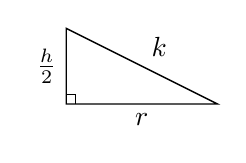
\begin{tikzpicture}[scale=0.8]
\draw[line width=0.5pt] (0,0) -- (2.4,0) -- (0,1.2) -- cycle; \draw[line width=0.4pt] (0,0.15)--(0.15,0.15)--(0.15,0);
\node[left] at (0,0.6) {$\frac{h}{2}$}; \node[below] at (1.2,0) {$r$}; \node[above right] at (1.2,0.6) {$k$};
\end{tikzpicture}}
% RVHS 2025 Promo Q1 solution diagram (conical tank with water)
\newcommand{\figRVHSsol}{\begin{tikzpicture}[scale=0.85]
\fill[blue!15] (-0.9,-1.5) -- (0,-3) -- (0.9,-1.5) arc[start angle=0,end angle=-180,x radius=0.9,y radius=0.15];
\draw[blue!50,fill=blue!8] (0,-1.5) ellipse (0.9 and 0.15);
\draw[c9] (0,0) ellipse (1.8 and 0.3); \draw[c9] (-1.8,0) -- (0,-3) -- (1.8,0);
\draw[c9aa] (0,0) -- (1.78,0); \node[above] at (0.9,0) {$3$};
\draw[c9aa] (-0.15,0) -- (-0.15,-3); \node[left] at (-0.15,-0.8) {$6$};
\draw[c9a] (0,-1.5) -- (0.88,-1.5); \node[above] at (0.45,-1.5) {$r$};
\draw[c9aa] (0.15,-1.5) -- (0.15,-3); \node[right] at (0.15,-2.2) {$h$};
\end{tikzpicture}}

\usepackage{multicol}
%% ---- change highlights turned OFF (28 Oct 2026, Maximus): macros keep content, no yellow ----
\definecolor{FLhl}{RGB}{255,240,0}
\protected\def\fhl#1{\ifmmode\text{#1}\else{#1}\fi}
\newcommand{\fhlm}[1]{\ensuremath{\displaystyle#1}}
\newcommand{\fhlmi}[1]{\ensuremath{#1}}
\newcommand{\fhlp}[1]{{#1}}
\newcommand{\flagi}[2]{{\setlength{\fboxsep}{1.5pt}\setlength{\fboxrule}{0.7pt}\fcolorbox{red}{white}{\textcolor{red}{\scriptsize\bfseries #1: #2}}}}
% block red note (own paragraph). #1 = flag id, #2 = severity, #3 = text
\newcommand{\flagb}[3]{\par\medskip\noindent{\setlength{\fboxsep}{3pt}\setlength{\fboxrule}{0.9pt}\fcolorbox{red}{red!6}{\parbox{\dimexpr\linewidth-2\fboxsep-2\fboxrule\relax}{\raggedright\color{red!70!black}\footnotesize\textbf{FLAG #1 [#2] --- for Maximus to review:} #3}}}\par\medskip}

%% ---- Chapter 15 (Vectors): packages, TikZ libraries and macros merged from vectors_draft.tex ----
\usepackage{tikz-3dplot}\usepackage{colortbl}\usetikzlibrary{arrows.meta,positioning,shapes.geometric,calc}
\providecommand{\vv}[1]{\mathbf{#1}}
\providecommand{\cv}[3]{\begin{pmatrix}#1\\#2\\#3\end{pmatrix}}
\providecommand{\need}[1]{{\color{blue!50!black}\textbf{Need:} #1}}
\providecommand{\sref}[1]{{\color{gray}\footnotesize\S#1}}
\providecommand{\vab}[1]{\overrightarrow{#1}}
\providecommand{\cvf}[3]{\begin{pmatrix}#1\\[1.6ex]#2\\[1.6ex]#3\end{pmatrix}}
\providecommand{\illus}{\textcolor{gray}{\footnotesize(illustration, checked)}}
\providecommand{\srcex}{}
\providecommand{\todo}[1]{\par\noindent\colorbox{yellow!30}{\parbox{\dimexpr\textwidth-2\fboxsep}{\small\textbf{DRAFT:} #1}}\par\smallskip}
\definecolor{Lcol}{RGB}{230,120,0}
%% ---- change highlighting (Vectors): \highlightfalse = ALL \hl/\hlm/\hlb/\hlf highlights OFF (approved 27 Oct 2026) ----
\definecolor{HLc}{RGB}{255,245,120}
\newif\ifhighlight\highlightfalse
\newcommand{\hl}[1]{\ifhighlight\colorbox{HLc}{#1}\else#1\fi}
\newcommand{\hlm}[1]{\ifhighlight\colorbox{HLc}{$\displaystyle#1$}\else\ensuremath{#1}\fi}
\newcommand{\hlb}[1]{\ifhighlight\colorbox{HLc}{\parbox{\dimexpr\linewidth-2\fboxsep\relax}{\centering#1}}\else#1\fi}
\newcommand{\hlf}[1]{\ifhighlight{\setlength{\fboxrule}{1.6pt}\setlength{\fboxsep}{2pt}\fcolorbox{orange!85!yellow}{white}{#1}}\else#1\fi}
\tikzset{pt/.style={circle,fill,inner sep=1.2pt},ar/.style={-{Stealth},thick}}
\begin{document}
\makeatletter\setbox0\vbox{\@starttoc{toc}}\makeatother
\pgfplotsset{mini/.style={width=4.4cm,height=3.6cm,axis lines=middle,ticks=none,clip=false,xlabel=$x$,ylabel=$y$,label style={font=\small},unbounded coords=jump,every axis x label/.style={at={(ticklabel* cs:1)},anchor=west},every axis y label/.style={at={(ticklabel* cs:1)},anchor=south}},
noax/.style={width=4.8cm,height=4.4cm,axis lines=none,ticks=none,clip=false,axis equal image}}
\newcommand{\Om}{\node[anchor=north east,inner sep=1pt] at (axis cs:0,0){$O$};}
\newcommand{\ptt}[1]{\addplot[black,only marks,mark=*,mark size=1.2pt] coordinates{#1};}
\newcommand{\exg}[2]{\par\noindent\begin{minipage}[c]{0.54\textwidth}#1\end{minipage}\hspace{2mm}\begin{minipage}[c]{0.42\textwidth}\raggedright#2\end{minipage}\par\medskip}
\newcommand{\cell}[2]{\begin{minipage}[t]{0.32\textwidth}\centering#2\\[-1mm]{\small #1}\end{minipage}}

%% ================================================================ SUMMARY 1
\clearpage\thispagestyle{empty}\null\clearpage\IfFileExists{notes_hw.tocextra}{\input{notes_hw.tocextra}}{} %FRONTTOC
\inchap{Systems of Linear Equations}
\section{Forming the Equations}
We read the context of the question and form equations depending on the context of the question.\par\smallskip
\exlab
\sys{a+b+c&=176\lb1\\0.85a+0.90b+0.95c&=161.80\lb2\\0.93a+0.95b+0.98c&=169.56\lb3}{a=32,\ b=44,\ c=100}
\exlab
The ``variables'' may be expressions. To find $x$, $y$ and $z$, use the given information to form the equations:
\sys{2x^{3}+3\ln y-\e^{z}&=18\lb1\\x^{3}-\ln y+2\e^{z}&=9\lb2\\x^{3}+2\ln y+\e^{z}&=11\lb3}{x^{3}=8,\ \ln y=1,\ \e^{z}=1}
\sidenote{It is technically still `linear' because we can think of $A=x^{3}$, $B=\ln y$, $C=\e^{z}$, which turns it into a linear system in $A$, $B$ and $C$. A truly nonlinear equation could look like $x^{2}+x+y^{2}+2y-3z^{3}-xz+xy=1$; it cannot be made linear this way, because $x$ appears as both $x^{2}$ and $x$, and there are product terms such as $xz$ and $xy$.}
\section{Special Case: Number of Equations \texorpdfstring{$>$}{>} Number of Variables}
Sometimes the number of equations is more than the number of variables, and the solution must satisfy all of the equations.\par\smallskip
\exlab
\sys{\lambda+\mu&=1\lb1\\2\lambda-\mu&=5\lb2}{\lambda=2,\ \mu=-1}
\topdisplay{\lambda+3\mu=-1\qquad\text{---\,(3)}}
Sometimes there may be no solution, e.g.\ skew lines in vectors. In this case, solve for $\lambda$ and $\mu$ using equations (1) and (2). Then sub into (3).
\begin{info}[title=Note]
Check (3): if LHS $=$ RHS, the equations are consistent; if LHS $\neq$ RHS, there is no solution.
\end{info}
\section{Special Case: Number of Equations \texorpdfstring{$<$}{<} Number of Variables}
Sometimes the number of equations is less than the number of variables, so there are infinitely many solutions \fhl{(if consistent)}.\par\smallskip
\exlab
\sys{x+y+z&=6\lb1\\x-y+2z&=5\lb2}{x=\tfrac{11}{2}-\tfrac32z,\ y=\tfrac12+\tfrac12z,\ z=z}
\begin{info}[title=Note]
Useful trick: in contextual questions, the variables are usually non-negative integers, $z\in\mathbb{Z}^{+}_{0}$, so use this to find the solution from the general solution.
\end{info}
When $z=z$, it means that there are infinitely many solutions, and $z$ can be any real value. So just sub that into $x$ and $y$ to get a correct solution.
\[\setlength{\arraycolsep}{10pt}\begin{array}{llll}z=-1:\ (7,0,-1)&z=0:\ (\tfrac{11}{2},\tfrac{1}{2},0)&z=1:\ \textcolor{blue}{(4,1,1)}&z=2:\ (\tfrac{5}{2},\tfrac{3}{2},2)\\[2pt]z=3:\ \textcolor{blue}{(1,2,3)}&z=4:\ (-\tfrac{1}{2},\tfrac{5}{2},4)&z=5:\ (-2,3,5)&z=6:\ (-\tfrac{7}{2},\tfrac{7}{2},6)\end{array}\]
\sidenote{We can use the GC table to find all these solutions.}\par
%% ================================================================ SUMMARY 2
\clearpage
\inchap{Inequalities}
\section{Solving Inequalities Graphically}
Some inequalities cannot be solved algebraically, so we sketch the graphs and read off the solution.\par
\begin{itemize}\setlength\itemsep{0pt}\setlength\parskip{0pt}
\item Rearrange to $\mathrm{f}(x)>0$, or compare $y=\mathrm{f}(x)$ with $y=\mathrm{g}(x)$.
\item Sketch on the GC; mark the intersections and the asymptotes.
\item Read off the $x$-values where the required graph is above or below.
\end{itemize}
\exlab
\topdisplay{\left|x^{2}-4\right|\leqslant\ln(x+3)}
\begin{center}\begin{tikzpicture}
\begin{axis}[width=0.85\linewidth,height=8cm,axis lines=middle,xmin=-3.6,xmax=3.4,ymin=-2.5,ymax=6,ticks=none,clip=false,xlabel=$x$,ylabel=$y$,label style={font=\normalsize}]
\addplot[blue,semithick,domain=-3.6:3.2,samples=300]{abs(x^2-4)};
\addplot[red,semithick,domain=-2.92:3.4,samples=300]{ln(x+3)};
\addplot[black,dashed,thin] coordinates{(-3,-2.5)(-3,6)};
\addplot[black,only marks,mark=*,mark size=1.3pt] coordinates{(-2,0)(2,0)(0,4)(0,1.0986)(1.5746,1.5197)(2.3840,1.6837)};
\node[font=\normalsize,anchor=north east] at (axis cs:0,0){$O$};
\node[font=\normalsize,anchor=north] at (axis cs:-2,-0.15){$(-2,0)$};
\node[font=\normalsize,anchor=north] at (axis cs:2,-0.8){$(2,0)$};
\node[font=\normalsize,anchor=south west] at (axis cs:0.05,4){$(0,4)$};
\node[font=\normalsize,anchor=north west] at (axis cs:0.05,1.05){$(0,\ln3)$};
\draw[thin,dotted] (axis cs:1.5746,1.5197)--(axis cs:1.5746,0);\node[font=\normalsize,anchor=north east] at (axis cs:1.62,-0.1){$1.57$};
\draw[thin,dotted] (axis cs:2.3840,1.6837)--(axis cs:2.3840,0);\node[font=\normalsize,anchor=north west] at (axis cs:2.34,-0.1){$2.38$};
\node[font=\normalsize,anchor=north] at (axis cs:-3,-2.5){$x=-3$};
\node[font=\normalsize,anchor=west] at (axis cs:3.0,5.4){$y=|x^{2}-4|$};
\node[font=\normalsize,anchor=west] at (axis cs:3.4,1.9){$y=\ln(x+3)$};
\end{axis}\end{tikzpicture}\end{center}
\gcl{intersections at $x=1.5746$, $x=2.3840$}
\cdisp{\therefore\ x=-2\ \ \text{or}\ \ 1.57\leqslant x\leqslant2.38}
\clearpage
\section{Sign Test Technique}
We solve rational inequalities by finding where the expression changes sign.\par
\begin{itemize}\setlength\itemsep{0pt}\setlength\parskip{0pt}
\item Make the right-hand side $0$.
\item Do \textbf{not} cross multiply unless the expression or bracket is always positive.
\item Expressions that are always positive can be divided across, e.g.\ a quadratic with discriminant $<0$ and positive leading coefficient: $x^{2}+2x+5=(x+1)^{2}+4>0$.
\end{itemize}
\exlab
\topdisplay{\frac{(x-1)(x-2)^{2}}{(x-3)(x-4)}\leqslant0}
\begin{center}\begin{tikzpicture}
\draw[dashed,-{Stealth[length=2mm]}](-0.3,0)--(10.3,0);
\foreach \p/\l in {2/1,4/2,6/3,8/4}{\draw(\p,0.12)--(\p,-0.12)node[below]{$\l$};}
\foreach \p/\s in {1/-,3/+,5/+,7/-,9/+}{\node at(\p,0.35){$\s$};}
\end{tikzpicture}\end{center}
\cdisp{&x=2:\ \text{numerator }=0\ \ (\text{included})\\
&x=3,\ x=4:\ \text{denominator }=0\ \ (\text{excluded})\\
&\therefore\ x\leqslant1\ \ \text{or}\ \ x=2\ \ \text{or}\ \ 3<x<4}
\sidenote{You can sketch the graph to check the answer.}\par
\begin{info}[title=Note]
Crossing a factor with an odd power changes the sign; crossing a factor with an even power keeps the sign the same.
\end{info}
\clearpage
\section{Common Substitutions}
Once an inequality in $x$ is solved, we can replace $x$ with an expression to deduce the solution of a related inequality.\par\smallskip
\begin{center}\renewcommand{\arraystretch}{1.5}
\begin{tabular}{|c|c|c|c|}\hline
 & \multicolumn{3}{c|}{\textbf{Original inequality}}\\\cline{2-4}
\textbf{Replace $x$ by} & $x>2$ & $x<-1$ & $-1<x<2$\\\Xhline{2pt}
$\e^{x}$ & $x>\ln2$ & no solution & $x<\ln2$\\\hline
$\ln x$ & $x>\e^{2}$ & $0<x<\e^{-1}$ & $\e^{-1}<x<\e^{2}$\\\hline
$-x$ & $x<-2$ & $x>1$ & $-2<x<1$\\\hline
$x+1$ & $x>1$ & $x<-2$ & $-2<x<1$\\\hline
$|x|$ & $x<-2$ or $x>2$ & no solution & $-2<x<2$\\\hline
$x^{2}$ & $x<-\sqrt2$ or $x>\sqrt2$ & no solution & $-\sqrt2<x<\sqrt2$\\\hline
$\dfrac1x$ & $\left(0<x<\tfrac12\right)$ & $(-1<x<0)$ & $\left(x<-1\text{ or }x>\tfrac12\right)$\\\hline
$\cos x$, $0\leqslant x\leqslant2\pi$ & (no solution) & (no solution) & $(0\leqslant x<\pi\text{ or }\pi<x\leqslant2\pi)$\\\hline
\end{tabular}\end{center}
\sidenote{Regardless of whatever substitution you use, using a graph will always work, but some can be solved without a graph.}\par
For $\dfrac1x$, $\sin x$ and $\cos x$, draw the graph to solve.\par\medskip
\noindent\begin{minipage}[t]{0.48\textwidth}
\exlab
\topdisplay{\frac1x>2,\quad \frac1x<-1,\quad -1<\frac1x<2}
\begin{center}\begin{tikzpicture}
\begin{axis}[width=\linewidth,height=6.5cm,axis lines=middle,xmin=-3,xmax=3,ymin=-3.5,ymax=3.5,ticks=none,clip=false,xlabel=$x$,ylabel=$y$]
\addplot[blue,semithick,domain=0.29:3,samples=80]{1/x};\addplot[blue,semithick,domain=-3:-0.29,samples=80]{1/x};
\addplot[red,dotted,thick,domain=-3:3]{2};\addplot[red,dotted,thick,domain=-3:3]{-1};\node[font=\scriptsize,anchor=north east] at (axis cs:0,0){$O$};\node[font=\tiny,anchor=south east] at (axis cs:0,2){$(0,2)$};\node[font=\tiny,anchor=north east] at (axis cs:0,-1){$(0,-1)$};
\node[font=\scriptsize,anchor=west] at (axis cs:3,2){$y=2$};\node[font=\scriptsize,anchor=west] at (axis cs:3,-1){$y=-1$};
\node[font=\scriptsize] at (axis cs:1.6,1.1){$y=\frac1x$};
\end{axis}\end{tikzpicture}\end{center}
\end{minipage}\hfill\begin{minipage}[t]{0.48\textwidth}
\exlab
\topdisplay{\cos x>\tfrac12,\quad \cos x<-\tfrac12,}\topdisplay{-\tfrac12<\cos x<\tfrac12,\quad 0\leqslant x\leqslant2\pi}
\begin{center}\begin{tikzpicture}
\begin{axis}[width=\linewidth,height=6.5cm,axis lines=middle,xmin=0,xmax=2.15*pi,ymin=-1.3,ymax=1.4,
  xtick={pi/2,pi,3*pi/2,2*pi},xticklabels={$\frac{\pi}{2}$,$\pi$,$\frac{3\pi}{2}$,$2\pi$},ytick={-1,-0.5,0.5,1},yticklabels={$-1$,$-\frac12$,$\frac12$,$1$},tick label style={font=\scriptsize},xlabel=$x$,ylabel=$y$]
\addplot[blue,semithick,domain=0:2*pi,samples=200]{cos(deg(x))};
\addplot[red,dotted,thick,domain=0:2*pi]{0.5};\addplot[red,dotted,thick,domain=0:2*pi]{-0.5};\node[font=\scriptsize,anchor=north east] at (axis cs:0,0){$O$};\addplot[black,only marks,mark=*,mark size=1pt] coordinates{(pi/2,0)(3*pi/2,0)(0,1)};\node[font=\tiny,anchor=south west] at (axis cs:pi/2,0){$(\frac{\pi}{2},0)$};\node[font=\tiny,anchor=north west] at (axis cs:3*pi/2,0){$(\frac{3\pi}{2},0)$};\node[font=\tiny,anchor=south west] at (axis cs:0,1){$(0,1)$};
\end{axis}\end{tikzpicture}\end{center}
\end{minipage}
%% ================================================================ SUMMARY 3
\clearpage
\inchap{Graphing Techniques}
\section{Key Features of a Curve}
Key features of a curve:
\begin{enumerate}[label=(\alph*)]
\item \exg{\textbf{$x$-intercepts:} let $y=0$.\par e.g.\ $y=x^{2}-1$: $x^{2}-1=0\Rightarrow x=\pm1$.}{\begin{tikzpicture}\begin{axis}[mini,xmin=-2,xmax=2,ymin=-1.6,ymax=3]
\addplot[blue,semithick,domain=-2:2,samples=80]{x^2-1};\ptt{(-1,0)(1,0)}\Om
\node[anchor=north east,inner sep=1pt] at (axis cs:-1,0){$(-1,0)$};\node[anchor=north west,inner sep=1pt] at (axis cs:1,0){$(1,0)$};\end{axis}\end{tikzpicture}}
\exg{\textbf{$y$-intercepts:} let $x=0$.\par e.g.\ $y=x+2$: $y=2$.}{\begin{tikzpicture}\begin{axis}[mini,xmin=-3,xmax=2,ymin=-1.5,ymax=4]
\addplot[blue,semithick,domain=-3:2]{x+2};\ptt{(0,2)}\Om
\node[anchor=north west,inner sep=1pt] at (axis cs:0.12,2.05){$(0,2)$};\end{axis}\end{tikzpicture}}

\item \textbf{Stationary points}, \fhl{when $\dfrac{\mathrm{d}y}{\mathrm{d}x}=0$.} Label upon request.

\exg{\textbf{Horizontal turning point:} $\dfrac{\mathrm{d}y}{\mathrm{d}x}=0$ (tangent horizontal).\par e.g.\ $y=-(x-1)^{2}+2$, maximum point $(1,2)$.}{\begin{tikzpicture}\begin{axis}[mini,xmin=-1.2,xmax=3.2,ymin=-1.5,ymax=3]
\addplot[blue,semithick,domain=-0.8:2.8,samples=80]{-(x-1)^2+2};\ptt{(1,2)}\Om
\node[anchor=south] at (axis cs:1,2){$(1,2)$};
\end{axis}\end{tikzpicture}}
\exg{\textbf{Vertical turning point:} $\dfrac{\mathrm{d}y}{\mathrm{d}x}$ undefined (tangent vertical).\par e.g.\ $x=(y-1)^{2}+1$, turning point $(1,1)$.}{\begin{tikzpicture}\begin{axis}[mini,xmin=-0.6,xmax=4,ymin=-1.2,ymax=3.2]
\addplot[blue,semithick,domain=-0.6:2.6,samples=80,variable=\t]({(t-1)^2+1},{t});\ptt{(1,1)}\Om
\node[anchor=east] at (axis cs:1,1){$(1,1)$};\end{axis}\end{tikzpicture}}

\clearpage
\item \textbf{Asymptotes}
\begin{enumerate}[label=(\roman*),leftmargin=2.5em]
\item \textbf{Vertical asymptotes.} If as $x\to k$, $y\to\pm\infty$, then $x=k$ is a vertical asymptote.\par\smallskip
{\renewcommand{\arraystretch}{1.3}\begin{tabular}{|>{\raggedright\arraybackslash}m{2.2cm}|>{\raggedright\arraybackslash}m{3.2cm}|>{\raggedright\arraybackslash}m{3.4cm}|>{\centering\arraybackslash}m{4.4cm}|}\hline
\textbf{Common Occurrence} & \textbf{Condition} & \textbf{Example and asymptote} & \textbf{Graph}\\\hline
Fractions & denominator $=0$ \fhl{\sidenote{(numerator $\neq0$)}} & $y=\dfrac{1}{x-1}$\par $x-1=0\Rightarrow x=1$\par $\therefore x=1$ is a vertical asymptote & \rule{0pt}{3.4cm}\begin{tikzpicture}\begin{axis}[mini,width=4cm,height=3.2cm,xmin=-2,xmax=4,ymin=-3,ymax=3]
\addplot[blue,semithick,domain=1.34:4,samples=80]{1/(x-1)};\addplot[blue,semithick,domain=-2:0.66,samples=80]{1/(x-1)};
\addplot[red,dashed] coordinates{(1,-3)(1,3)};\Om\node[anchor=north,red,font=\small] at (axis cs:1,-3){$x=1$};\end{axis}\end{tikzpicture}\\\hline
Logarithmic graphs & inside $\ln=0$ & $y=\ln(x-2)$\par $x-2=0\Rightarrow x=2$\par $\therefore x=2$ is a vertical asymptote & \rule{0pt}{3.4cm}\begin{tikzpicture}\begin{axis}[mini,width=4cm,height=3.2cm,xmin=-0.5,xmax=6,ymin=-3,ymax=2]
\addplot[blue,semithick,domain=2.05:6,samples=100]{ln(x-2)};\addplot[red,dashed] coordinates{(2,-3)(2,2)};\Om
\node[anchor=north,red,font=\small] at (axis cs:2,-3){$x=2$};\end{axis}\end{tikzpicture}\\\hline
Tangent graphs & inside $\tan=\dfrac{\pi}{2}+k\pi$, $k\in\mathbb{Z}$ & $y=\tan x$\par $x=\pm\dfrac{\pi}{2},\ \pm\dfrac{3\pi}{2},\dots$ & \rule{0pt}{3.4cm}\begin{tikzpicture}\begin{axis}[mini,width=4cm,height=3.2cm,xmin=-2.6,xmax=2.6,ymin=-3,ymax=3]
\addplot[blue,semithick,domain=-1.25:1.25,samples=80]{tan(deg(x))};\addplot[red,dashed] coordinates{(-1.5708,-3)(-1.5708,3)};\addplot[red,dashed] coordinates{(1.5708,-3)(1.5708,3)};\Om
\node[anchor=north,red,font=\small] at (axis cs:-1.57,-3){$x=-\frac{\pi}{2}$};\node[anchor=north,red,font=\small] at (axis cs:1.57,-3){$x=\frac{\pi}{2}$};\end{axis}\end{tikzpicture}\\\hline
\end{tabular}}
\item \textbf{Horizontal asymptotes.} As $x\to\pm\infty$, if $y\to k$, then $y=k$ is a horizontal asymptote.
\begin{itemize}
\item \textcolor{red}{To find horizontal asymptotes, one should sub in $x\to\pm\infty$ into the equation. This is the only foolproof way to do it.}
\item \textcolor{red}{A curve \textbf{CAN} intersect its horizontal asymptote.}
\end{itemize}
\noindent\begin{minipage}[t]{0.48\textwidth}\centering\begin{tikzpicture}\begin{axis}[mini,width=6.4cm,height=4cm,xmin=-13,xmax=13,ymin=-0.5,ymax=1.3]
\addplot[blue,semithick,domain=-13:13,samples=300]{x==0?1:sin(deg(x))/x};\addplot[red,dashed] coordinates{(-13,0)(13,0)};\Om
\addplot[only marks,mark=o,mark size=1.4pt,fill=white] coordinates{(0,1)};\node[anchor=south west,font=\small] at (axis cs:0.3,1){$(0,1)$};\node[anchor=north,red,font=\small] at (axis cs:-10,-0.2){$y=0$};\draw[->,thick,black!70](axis cs:6.5,0.45)--(axis cs:11.5,0.15);\node[anchor=south,font=\small] at (axis cs:8.5,0.5){as $x\to\pm\infty$, $y\to0$};\end{axis}\end{tikzpicture}\par{\small e.g.\ $y=\dfrac{\sin x}{x}$: curve crosses $y=0$}\end{minipage}\hfill
\begin{minipage}[t]{0.48\textwidth}\centering\begin{tikzpicture}\begin{axis}[mini,width=6.4cm,height=4cm,xmin=-1.5,xmax=5,ymin=-0.6,ymax=7]
\addplot[blue,semithick,domain=-1.3:5,samples=100]{3+exp(-x)};\addplot[red,dashed] coordinates{(-1.5,3)(5,3)};\Om
\addplot[black,only marks,mark=*,mark size=1.2pt] coordinates{(0,4)};\node[anchor=south west,font=\small] at (axis cs:0.05,4.05){$(0,4)$};\node[anchor=north,red,font=\small] at (axis cs:4.3,2.95){$y=3$};\draw[->,thick,black!70](axis cs:1.6,4.4)--(axis cs:4.2,3.4);\node[anchor=south west,font=\small] at (axis cs:1.8,4.5){as $x\to\infty$, $y\to3$};\end{axis}\end{tikzpicture}\par{\small e.g.\ $y=3+\e^{-x}$}\end{minipage}\par\vspace{1.5cm}
\newpage
\noindent\textbf{Useful trick to find horizontal asymptotes}\par\smallskip
For rational functions $\dfrac{P(x)}{Q(x)}$:\par\smallskip
{\renewcommand{\arraystretch}{1.3}\setlength{\tabcolsep}{4pt}\centering\begin{tabular}{|>{\raggedright\arraybackslash}m{3.3cm}|>{\raggedright\arraybackslash}m{3.6cm}|>{\raggedright\arraybackslash}m{2.4cm}|>{\centering\arraybackslash}m{4cm}|}\hline
\textbf{Case} & \textbf{Horizontal asymptote} & \textbf{Example} & \textbf{Graph}\\\hline
numerator power $>$ denominator power & no horizontal asymptote & $y=\dfrac{x^{2}}{x-1}$ & \rule{0pt}{3.1cm}\begin{tikzpicture}\begin{axis}[mini,width=3.8cm,height=3cm,xmin=-3,xmax=4,ymin=-6,ymax=8]
\addplot[blue,semithick,domain=1.15:4,samples=80]{x^2/(x-1)};\addplot[blue,semithick,domain=-3:0.88,samples=80]{x^2/(x-1)};
\addplot[red,dashed] coordinates{(1,-6)(1,8)};\addplot[red,dashed,domain=-3:4]{x+1};\Om\node[anchor=north,red,font=\small] at (axis cs:1,-6){$x=1$};\node[anchor=west,red,font=\small] at (axis cs:4,5){$y=x+1$};\end{axis}\end{tikzpicture}\\\hline
numerator power $<$ denominator power & $y=0$ & $y=\dfrac{1}{x^{2}+1}$ & \rule{0pt}{2.6cm}\begin{tikzpicture}\begin{axis}[mini,width=3.8cm,height=2.6cm,xmin=-3.5,xmax=3.5,ymin=-0.3,ymax=1.4]
\addplot[blue,semithick,domain=-3.5:3.5,samples=80]{1/(x^2+1)};\Om\end{axis}\end{tikzpicture}\\\hline
numerator power $=$ denominator power & ratio of coefficients of highest power & $y=\dfrac{2x+1}{x-1}$\par $y=2$ & \rule{0pt}{3.1cm}\begin{tikzpicture}\begin{axis}[mini,width=3.8cm,height=3cm,xmin=-4,xmax=5,ymin=-5,ymax=8]
\addplot[blue,semithick,domain=1.4:5,samples=80]{(2*x+1)/(x-1)};\addplot[blue,semithick,domain=-4:0.6,samples=80]{(2*x+1)/(x-1)};
\addplot[red,dashed] coordinates{(1,-5)(1,8)};\addplot[red,dashed] coordinates{(-4,2)(5,2)};\Om
\node[anchor=north,red,font=\small] at (axis cs:1,-5){$x=1$};\node[anchor=west,red,font=\small] at (axis cs:5,2){$y=2$};\end{axis}\end{tikzpicture}\\\hline
\end{tabular}\par}
\item \textbf{Oblique asymptotes.} An asymptote of the form $y=mx+c$, $m\neq0$.\par
Graphs with oblique asymptotes come in the form $y=mx+c+\mathrm{g}(x)$, where $\mathrm{g}(x)\to0$ as $x\to\pm\infty$; the oblique asymptote is $y=mx+c$.\par\smallskip
\noindent\begin{minipage}[t]{0.48\textwidth}\centering
\begin{tikzpicture}\begin{axis}[mini,width=5.2cm,height=4.4cm,xmin=-4,xmax=7,ymin=-12,ymax=18]
\addplot[blue,semithick,domain=2.2:7,samples=100]{2*x+1+3/(x-2)};\addplot[blue,semithick,domain=-4:1.75,samples=100]{2*x+1+3/(x-2)};
\addplot[red,dashed] coordinates{(2,-12)(2,18)};\addplot[red,dashed,domain=-4:7]{2*x+1};\Om
\node[anchor=north,red,font=\small] at (axis cs:2,-12){$x=2$};\node[anchor=west,red,font=\small] at (axis cs:7,15){$y=2x+1$};\end{axis}\end{tikzpicture}\par
e.g.\ $y=2x+1+\dfrac{3}{x-2}$\end{minipage}\hfill
\begin{minipage}[t]{0.48\textwidth}\centering
\begin{tikzpicture}\begin{axis}[mini,width=5.2cm,height=4.4cm,xmin=-2,xmax=4,ymin=-8,ymax=10]
\addplot[blue,semithick,domain=-1.6:4,samples=100]{3*x-5+exp(-x)};
\addplot[red,dashed,domain=-1:4]{3*x-5};\Om
\node[anchor=west,red,font=\small] at (axis cs:4,7){$y=3x-5$};\end{axis}\end{tikzpicture}\par
e.g.\ $y=3x-5+\e^{-x}$\end{minipage}\par\medskip
\begin{info}[title=Note]
For parametric curves, oblique asymptotes (if they exist) can \fhl{usually} be found via the cartesian equation.
\end{info}
\end{enumerate}
\end{enumerate}
\clearpage
\section{Graphs of Rational Functions}
Two common shapes for each type.\par\medskip
{\renewcommand{\arraystretch}{1.2}\centering\begin{tabular}{|>{\raggedright\arraybackslash}m{3.7cm}|>{\centering\arraybackslash}m{5.6cm}|>{\centering\arraybackslash}m{5.6cm}|}\hline
\textbf{Type and form} & \textbf{Shape 1} & \textbf{Shape 2}\\\hline
\textbf{Linear / linear}\par\smallskip $y=\dfrac{Ax+B}{Cx+D}$\par Horizontal asymptote: $y=\dfrac{A}{C}$\par Vertical asymptote: $x=-\dfrac{D}{C}$ & \rule{0pt}{4ex}\begin{tikzpicture}\begin{axis}[mini,width=5.4cm,height=4.6cm,xmin=-3,xmax=4,ymin=-4,ymax=5]
\addplot[blue,semithick,domain=1.5:4,samples=80]{(x+1)/(x-1)};\addplot[blue,semithick,domain=-3:0.6,samples=80]{(x+1)/(x-1)};
\addplot[red,dashed] coordinates{(1,-4)(1,5)};\addplot[red,dashed] coordinates{(-3,1)(4,1)};\Om
\node[anchor=north,red,font=\small] at (axis cs:1,-4){$x=1$};\node[anchor=west,red,font=\small] at (axis cs:4,1){$y=1$};\addplot[black,only marks,mark=*,mark size=1.2pt] coordinates{(-1,0)(0,-1)};\node[anchor=north east,font=\small,inner sep=1pt] at (axis cs:-1.05,-0.1){$(-1,0)$};\node[anchor=north west,font=\small,inner sep=1pt] at (axis cs:0.1,-1.1){$(0,-1)$};\end{axis}\end{tikzpicture}\par{\small $y=\dfrac{x+1}{x-1}$} & \begin{tikzpicture}\begin{axis}[mini,width=5.4cm,height=4.6cm,xmin=-4,xmax=3,ymin=-4,ymax=5]
\addplot[blue,semithick,domain=-0.6:3,samples=80]{(x-1)/(x+1)};\addplot[blue,semithick,domain=-4:-1.5,samples=80]{(x-1)/(x+1)};
\addplot[red,dashed] coordinates{(-1,-4)(-1,5)};\addplot[red,dashed] coordinates{(-4,1)(3,1)};\Om
\node[anchor=north,red,font=\small] at (axis cs:-1,-4){$x=-1$};\node[anchor=west,red,font=\small] at (axis cs:3,1){$y=1$};\addplot[black,only marks,mark=*,mark size=1.2pt] coordinates{(1,0)(0,-1)};\node[anchor=north west,font=\small,inner sep=1pt] at (axis cs:1.1,-0.1){$(1,0)$};\node[anchor=north east,font=\small,inner sep=1pt] at (axis cs:-0.1,-1.1){$(0,-1)$};\end{axis}\end{tikzpicture}\par{\small $y=\dfrac{x-1}{x+1}$}\\\hline
\textbf{Quadratic / linear}\par\smallskip $y=\dfrac{ax^{2}+bx+c}{dx+e}$\par $=Ax+B+\dfrac{C}{dx+e}$\par Oblique asymptote: $y=Ax+B$\par Vertical asymptote: $x=-\dfrac{e}{d}$ & \rule{0pt}{4ex}\begin{tikzpicture}\begin{axis}[mini,width=5.4cm,height=4.6cm,xmin=-3,xmax=4.5,ymin=-5,ymax=8]
\addplot[blue,semithick,domain=1.17:4.5,samples=100]{x+1+1/(x-1)};\addplot[blue,semithick,domain=-3:0.85,samples=100]{x+1+1/(x-1)};
\addplot[red,dashed] coordinates{(1,-5)(1,8)};\addplot[red,dashed,domain=-3:4.5]{x+1};\Om
\node[anchor=north,red,font=\small] at (axis cs:1,-5){$x=1$};\node[anchor=west,red,font=\small] at (axis cs:4.5,5.5){$y=x+1$};\addplot[black,only marks,mark=*,mark size=1.2pt] coordinates{(0,0)(2,4)};\node[anchor=north west,font=\small,inner sep=1pt] at (axis cs:2.1,3.9){$(2,4)$};\end{axis}\end{tikzpicture}\par{\small 2 turning points\par $y=x+1+\dfrac{1}{x-1}$\quad $\left(\dfrac{Cd}{A}>0\right)$} & \begin{tikzpicture}\begin{axis}[mini,width=5.4cm,height=4.6cm,xmin=-3,xmax=4.5,ymin=-5,ymax=8]
\addplot[blue,semithick,domain=1.12:4.5,samples=100]{x+1-1/(x-1)};\addplot[blue,semithick,domain=-3:0.88,samples=100]{x+1-1/(x-1)};
\addplot[red,dashed] coordinates{(1,-5)(1,8)};\addplot[red,dashed,domain=-3:4.5]{x+1};\Om
\node[anchor=north,red,font=\small] at (axis cs:1,-5){$x=1$};\node[anchor=west,red,font=\small] at (axis cs:4.5,5.5){$y=x+1$};\addplot[black,only marks,mark=*,mark size=1.2pt] coordinates{(0,2)(-1.414,0)(1.414,0)};\node[anchor=east,font=\small,inner sep=1pt] at (axis cs:-0.1,2.3){$(0,2)$};\node[anchor=north east,font=\small,inner sep=1pt] at (axis cs:-1.45,-0.1){$(-1.41,0)$};\node[anchor=north west,font=\small,inner sep=1pt] at (axis cs:1.5,-0.1){$(1.41,0)$};\end{axis}\end{tikzpicture}\par{\small No turning points\par $y=x+1-\dfrac{1}{x-1}$\quad $\left(\dfrac{Cd}{A}<0\right)$}\\\hline
\textbf{Linear / quadratic}\par\smallskip $y=\dfrac{ax+b}{cx^{2}+dx+e}$\par Horizontal asymptote: $y=0$\par Vertical asymptotes: solve $cx^{2}+dx+e=0$ (possibly no roots) & \rule{0pt}{4ex}\begin{tikzpicture}\begin{axis}[mini,width=5.4cm,height=4.6cm,xmin=-3,xmax=3,ymin=-4,ymax=4]
\foreach \a/\b in {-3/-1.12,-0.89/0.89,1.12/3}{\addplot[blue,semithick,domain=\a:\b,samples=80]{x/((x-1)*(x+1))};}
\addplot[red,dashed] coordinates{(1,-4)(1,4)};\addplot[red,dashed] coordinates{(-1,-4)(-1,4)};\Om
\node[anchor=north,red,font=\small] at (axis cs:-1,-4){$x=-1$};\node[anchor=north,red,font=\small] at (axis cs:1,-4){$x=1$};\end{axis}\end{tikzpicture}\par{\small $y=\dfrac{x}{(x-1)(x+1)}$} & \begin{tikzpicture}\begin{axis}[mini,width=5.8cm,height=6.2cm,xmin=-3,xmax=9,ymin=-2.5,ymax=3.2]
\addplot[blue,semithick,domain=-3:-1.556,samples=80]{(x-2)/((x-1)*(x+1))};\addplot[blue,semithick,domain=-0.476:0.788,samples=100]{(x-2)/((x-1)*(x+1))};\addplot[blue,semithick,domain=1.156:9,samples=200]{(x-2)/((x-1)*(x+1))};
\addplot[red,dashed] coordinates{(1,-2.5)(1,3.2)};\addplot[red,dashed] coordinates{(-1,-2.5)(-1,3.2)};\Om
\addplot[black,only marks,mark=*,mark size=1.2pt] coordinates{(0,2)(2,0)(3.732,0.134)(0.268,1.866)};
\node[anchor=east,font=\small,inner sep=1pt] at (axis cs:-0.1,2.0){$(0,2)$};\node[anchor=north,font=\small,inner sep=2pt] at (axis cs:2,-0.05){$(2,0)$};
\node[anchor=south,font=\small,inner sep=3pt] at (axis cs:4.3,0.15){$(3.73,0.134)$};\node[anchor=west,font=\small,inner sep=1pt] at (axis cs:1.2,1.87){$(0.268,1.87)$};\draw[gray,thin](axis cs:0.33,1.87)--(axis cs:1.2,1.87);
\node[anchor=north,red,font=\small] at (axis cs:-1,-2.5){$x=-1$};\node[anchor=north,red,font=\small] at (axis cs:1,-2.5){$x=1$};\end{axis}\end{tikzpicture}\par{\small $y=\dfrac{x-2}{(x-1)(x+1)}$}\\\hline
\end{tabular}\par}

\clearpage
\section{Symmetry}
\noindent\begin{minipage}[t]{0.48\textwidth}
\textbf{Even functions:} $\mathrm{f}(-x)=\mathrm{f}(x)$.\par The graph is symmetric about the $y$-axis (line of symmetry $x=0$, dotted).\par\smallskip\centering
\begin{tikzpicture}\begin{axis}[mini,width=3.9cm,height=3.5cm,xmin=-2,xmax=2,ymin=-0.4,ymax=3.4]
\addplot[blue,semithick,domain=-1.8:1.8,samples=80]{x^2};\addplot[black,dotted,thick] coordinates{(0,-0.4)(0,3.4)};\Om\end{axis}\end{tikzpicture}\hfill
\begin{tikzpicture}\begin{axis}[mini,width=3.9cm,height=3.5cm,xmin=-3.3,xmax=3.3,ymin=-1.3,ymax=1.3]
\addplot[blue,semithick,domain=-3.14:3.14,samples=100]{cos(deg(x))};\addplot[black,dotted,thick] coordinates{(0,-1.3)(0,1.3)};\Om\end{axis}\end{tikzpicture}\par
{\small e.g.\ $y=x^{2}$\hspace{2.2cm}e.g.\ $y=\cos x$}
\end{minipage}\hfill\vrule\hfill
\begin{minipage}[t]{0.48\textwidth}
\textbf{Odd functions:} $\mathrm{f}(-x)=-\mathrm{f}(x)$.\par The graph is symmetric about the origin.\par\smallskip
\begin{minipage}[c]{0.4\linewidth}e.g.\ $y=x^{3}-x$\end{minipage}\hfill\begin{minipage}[c]{0.58\linewidth}\centering\begin{tikzpicture}\begin{axis}[mini,width=3.9cm,height=3.4cm,xmin=-2,xmax=2,ymin=-2.5,ymax=2.5]
\addplot[blue,semithick,domain=-1.6:1.6,samples=80]{x^3-x};\Om\end{axis}\end{tikzpicture}\end{minipage}\par\medskip
\textbf{Symmetry about $y=x$:} swapping $x$ and $y$ gives the same equation.\par\smallskip
\begin{minipage}[c]{0.4\linewidth}e.g.\ $y=\dfrac{1}{x}$\par ($xy=1$)\end{minipage}\hfill\begin{minipage}[c]{0.58\linewidth}\centering\begin{tikzpicture}\begin{axis}[mini,width=3.9cm,height=3.4cm,xmin=-3,xmax=3,ymin=-3,ymax=3]
\addplot[blue,semithick,domain=0.34:3,samples=60]{1/x};\addplot[blue,semithick,domain=-3:-0.34,samples=60]{1/x};\addplot[black,dotted,thick,domain=-3:3]{x};\node[anchor=west,font=\small] at (axis cs:2.6,2.8){$y=x$};\Om\end{axis}\end{tikzpicture}\end{minipage}
\end{minipage}\par\bigskip
\section{Basic Graphs}
\pgfplotsset{bg/.style={mini,width=4.2cm,height=2.75cm}}
{\renewcommand{\cell}[2]{\begin{minipage}[t]{0.29\textwidth}\centering\vspace{1mm}#2\\[-1mm]{\small #1}\vspace{1mm}\end{minipage}}\centering\begin{tabular}{|c|c|c|}\hline
\cell{Linear $y=x+1$}{\begin{tikzpicture}\begin{axis}[bg,xmin=-2.5,xmax=2,ymin=-1.5,ymax=3]\addplot[blue,semithick,domain=-2.5:2]{x+1};\ptt{(-1,0)(0,1)}\Om\node[anchor=south east,font=\small] at (axis cs:-1.1,0){$(-1,0)$};\node[anchor=west,font=\small] at (axis cs:0.1,0.9){$(0,1)$};\end{axis}\end{tikzpicture}} &
\cell{Quadratic $y=x^{2}-1$}{\begin{tikzpicture}\begin{axis}[bg,xmin=-2,xmax=2,ymin=-1.5,ymax=3]\addplot[blue,semithick,domain=-2:2]{x^2-1};\ptt{(-1,0)(1,0)(0,-1)}\Om\node[anchor=north east,font=\small] at (axis cs:-1,0){$(-1,0)$};\node[anchor=north west,font=\small] at (axis cs:1,0){$(1,0)$};\node[anchor=north west,font=\small] at (axis cs:0,-1){$(0,-1)$};\end{axis}\end{tikzpicture}} &
\cell{Cubic $y=x^{3}-x$}{\begin{tikzpicture}\begin{axis}[bg,xmin=-2,xmax=2,ymin=-2,ymax=2]\addplot[blue,semithick,domain=-1.55:1.55]{x^3-x};\ptt{(-1,0)(1,0)}\Om\node[anchor=south east,font=\small] at (axis cs:-1.05,0.1){$(-1,0)$};\node[anchor=north west,font=\small] at (axis cs:1.05,-0.1){$(1,0)$};\end{axis}\end{tikzpicture}}\\\hline
\cell{Exponential $y=\e^{x}$}{\begin{tikzpicture}\begin{axis}[bg,xmin=-3,xmax=2,ymin=-0.8,ymax=4]\addplot[blue,semithick,domain=-3:1.35]{exp(x)};\ptt{(0,1)}\Om\node[anchor=south east,font=\small] at (axis cs:0,1){$(0,1)$};\node[anchor=north,font=\small] at (axis cs:-2,-0.1){$y\to0$};\end{axis}\end{tikzpicture}} &
\cell{Logarithm $y=\ln x$}{\begin{tikzpicture}\begin{axis}[bg,xmin=-0.8,xmax=4,ymin=-3,ymax=2]\addplot[blue,semithick,domain=0.05:4,samples=100]{ln(x)};\ptt{(1,0)}\Om\node[anchor=north west,font=\small] at (axis cs:1,0){$(1,0)$};\node[anchor=east,font=\small,red] at (axis cs:0,-2.4){$x=0$};\end{axis}\end{tikzpicture}} &
\cell{Reciprocal $y=\frac1x$}{\begin{tikzpicture}\begin{axis}[bg,xmin=-3,xmax=3,ymin=-3,ymax=3]\addplot[blue,semithick,domain=0.33:3]{1/x};\addplot[blue,semithick,domain=-3:-0.33]{1/x};\Om\end{axis}\end{tikzpicture}}\\\hline
\cell{$y=\sin x$}{\begin{tikzpicture}\begin{axis}[bg,xmin=-3.6,xmax=3.6,ymin=-1.5,ymax=1.6]\addplot[blue,semithick,domain=-3.3:3.3,samples=100]{sin(deg(x))};\ptt{(-3.1416,0)(3.1416,0)}\Om\node[anchor=north,font=\small] at (axis cs:-3.14,0){$-\pi$};\node[anchor=north,font=\small] at (axis cs:3.14,0){$\pi$};\end{axis}\end{tikzpicture}} &
\cell{$y=\cos x$}{\begin{tikzpicture}\begin{axis}[bg,xmin=-3.6,xmax=3.6,ymin=-1.5,ymax=1.6]\addplot[blue,semithick,domain=-3.3:3.3,samples=100]{cos(deg(x))};\ptt{(0,1)(-1.5708,0)(1.5708,0)}\Om\node[anchor=south west,font=\small] at (axis cs:0,1){$(0,1)$};\node[anchor=north,font=\small] at (axis cs:-1.9,-0.05){$-\frac{\pi}{2}$};\node[anchor=south west,font=\small] at (axis cs:1.57,0){$\frac{\pi}{2}$};\end{axis}\end{tikzpicture}} &
\cell{$y=\tan x$}{\begin{tikzpicture}\begin{axis}[bg,xmin=-2.4,xmax=2.4,ymin=-3,ymax=3]\addplot[blue,semithick,domain=-1.25:1.25,samples=80]{tan(deg(x))};\addplot[red,dashed] coordinates{(-1.5708,-3)(-1.5708,3)};\addplot[red,dashed] coordinates{(1.5708,-3)(1.5708,3)};\Om\node[anchor=north,red,font=\small] at (axis cs:-1.57,-3){$x=-\frac{\pi}{2}$};\node[anchor=north,red,font=\small] at (axis cs:1.57,-3){$x=\frac{\pi}{2}$};\end{axis}\end{tikzpicture}}\\\hline
\cell{$y=\sin^{-1}x$}{\begin{tikzpicture}\begin{axis}[bg,xmin=-1.8,xmax=1.8,ymin=-2,ymax=2]\addplot[blue,semithick,domain=-1:1,samples=100]{rad(asin(x))};\ptt{(-1,-1.5708)(1,1.5708)}\Om\node[anchor=north,font=\small] at (axis cs:-1,-1.6){$(-1,-\frac{\pi}{2})$};\node[anchor=south,font=\small] at (axis cs:1,1.6){$(1,\frac{\pi}{2})$};\end{axis}\end{tikzpicture}} &
\cell{$y=\cos^{-1}x$}{\begin{tikzpicture}\begin{axis}[bg,xmin=-1.8,xmax=1.8,ymin=-0.6,ymax=3.6]\addplot[blue,semithick,domain=-1:1,samples=100]{rad(acos(x))};\ptt{(-1,3.1416)(1,0)(0,1.5708)}\Om\node[anchor=south,font=\small] at (axis cs:-1,3.14){$(-1,\pi)$};\node[anchor=north,font=\small] at (axis cs:1,0){$(1,0)$};\node[anchor=west,font=\small] at (axis cs:0.1,1.75){$(0,\frac{\pi}{2})$};\end{axis}\end{tikzpicture}} &
\cell{$y=\tan^{-1}x$}{\begin{tikzpicture}\begin{axis}[bg,xmin=-4,xmax=4,ymin=-2.2,ymax=2.2]\addplot[blue,semithick,domain=-4:4,samples=100]{rad(atan(x))};\addplot[red,dashed] coordinates{(-4,1.5708)(4,1.5708)};\addplot[red,dashed] coordinates{(-4,-1.5708)(4,-1.5708)};\Om\node[anchor=south,red,font=\small] at (axis cs:-2.5,1.57){$y=\frac{\pi}{2}$};\node[anchor=north,red,font=\small] at (axis cs:2.5,-1.57){$y=-\frac{\pi}{2}$};\end{axis}\end{tikzpicture}}\\\hline
\end{tabular}\par}

\clearpage
\section{Parametric Equations}
A curve $C$ can be described by giving both coordinates in terms of a parameter $t$:
\topdisplay{x=x(t),\quad y=y(t),\quad t\in T}
\exg{\exlab $x=2\cos t+1,\ \ y=3\sin t-2,\ \ 0\leqslant t\leqslant\pi$\par\smallskip
$t=0$: $(3,-2)$\quad $t=\frac{\pi}{2}$: $(1,1)$\quad $t=\pi$: $(-1,-2)$\par
$x=0$: $\left(0,\tfrac{3\sqrt3}{2}-2\right)$\par $y=0$: $\left(1\pm\tfrac{2\sqrt5}{3},0\right)$}
{\begin{tikzpicture}\begin{axis}[mini,width=6.6cm,height=5.4cm,xmin=-1.8,xmax=3.8,ymin=-2.6,ymax=1.6]
\addplot[blue,semithick,domain=0:180,samples=100]({2*cos(x)+1},{3*sin(x)-2});\addplot[black,only marks,mark=*,mark size=1.4pt] coordinates{(3,-2)(-1,-2)(1,1)};\Om
\node[anchor=north,font=\small] at (axis cs:3,-2){$(3,-2)$};\node[anchor=north,font=\small] at (axis cs:-1,-2){$(-1,-2)$};\node[anchor=south,font=\small] at (axis cs:1,1){$(1,1)$};
\end{axis}\end{tikzpicture}}
\begin{info}[title={CAUTION: sketching from parametric equations}]
\textbf{ALWAYS take note of the range of $t$ when sketching graphs.} The restriction on $t$ decides which part of the curve exists: above, $0\leqslant t\leqslant\pi$ gives only the upper half of the ellipse, with endpoints $(3,-2)$ and $(-1,-2)$, not the whole ellipse.
\end{info}
\subsection{Finding the Cartesian Equation}
The cartesian equation of $C$ is an equation without the parameter $t$. Common techniques:\par\smallskip
\textbf{\textcircled{\scriptsize1} Make $t$ the subject.}\quad e.g.\ $x=2t-1$, $y=3t^{2}+\e^{t}$, $t\in\mathbb{R}$
\cdisp{t&=\frac{x+1}{2}\\ y&=3\left(\frac{x+1}{2}\right)^{2}+\e^{\frac{x+1}{2}}}
\textbf{\textcircled{\scriptsize2} Trigo identity formulas.}\quad e.g.\ $x=2\cos t+1$, $y=3\sin t-2$, $0\leqslant t\leqslant\pi$
\cdisp{\cos t=\frac{x-1}{2},\quad \sin t&=\frac{y+2}{3}\\ \cos^{2}t+\sin^{2}t&=1\\ \frac{(x-1)^{2}}{4}+\frac{(y+2)^{2}}{9}&=1,\quad y\geqslant-2}
\textbf{\textcircled{\scriptsize3} Others.}\quad e.g.\ $x=t-\dfrac1t$, $y=t+\dfrac1t$, $t\neq0$
\cdisp{y+x=2t,\quad y-x&=\frac{2}{t}\\ (y+x)(y-x)&=4\\ y^{2}-x^{2}&=4}
\textcolor{red}{Note: Avoid finding the cartesian eqn if the question did not ask you to.}
\subsection{Asymptotes (Parametric Equations)}
\begin{itemize}
\item Find (if possible) $t\to t_0$ such that $x\to x_0$, $y\to\pm\infty$ (vertical asymptote $x=x_0$), or $y\to y_0$, $x\to\pm\infty$ (horizontal asymptote $y=y_0$).
\item Oblique asymptotes (if they exist) can \fhl{usually} be found via the cartesian equation.
\end{itemize}
\exg{\exlab $x=\dfrac{1}{t-1}$, \ $y=2t$, \ $t\neq1$
\cdisp{&\text{As }t\to\pm\infty,\ x\to0,\ y\to\pm\infty\\ &\therefore\ x=0\text{ is a vertical asymptote}\\ &\text{As }t\to1,\ x\to\pm\infty,\ y\to2\\ &\therefore\ y=2\text{ is a horizontal asymptote}}}{\begin{tikzpicture}\begin{axis}[mini,xmin=-4,xmax=4,ymin=-3,ymax=7]
\addplot[blue,semithick,domain=0.35:4,samples=100]{2+2/x};\addplot[blue,semithick,domain=-4:-0.42,samples=100]{2+2/x};
\addplot[red,dashed] coordinates{(-4,2)(4,2)};\addplot[red,dashed] coordinates{(0,-3)(0,7)};\addplot[black,only marks,mark=*,mark size=1.2pt] coordinates{(-1,0)};\Om
\node[anchor=north east,font=\small,inner sep=1pt] at (axis cs:-1,-0.1){$(-1,0)$};\node[anchor=west,red,font=\small] at (axis cs:4,2){$y=2$};\node[anchor=north west,red,font=\small] at (axis cs:0.1,-3){$x=0$};\end{axis}\end{tikzpicture}}
\exg{\textbf{Oblique asymptotes.} \fhl{Is not usually} \fhl{found from the} \fhl{parametric form}; find the cartesian equation first.\par e.g.\ $x=2\sec\theta$, \ $y=3\tan\theta$
\cdisp{\sec^{2}\theta-\tan^{2}\theta&=1\\ \frac{x^{2}}{4}-\frac{y^{2}}{9}&=1}
Oblique asymptotes: $y=\pm\dfrac{3}{2}x$}{\begin{tikzpicture}\begin{axis}[mini,xmin=-6,xmax=6,ymin=-7,ymax=7]
\addplot[blue,semithick,domain=-1.5:1.5,samples=80,variable=\t]({2*cosh(t)},{3*sinh(t)});\addplot[blue,semithick,domain=-1.5:1.5,samples=80,variable=\t]({-2*cosh(t)},{3*sinh(t)});
\addplot[red,dashed,domain=-4.6:4.6]{1.5*x};\addplot[red,dashed,domain=-4.6:4.6]{-1.5*x};\Om
\node[anchor=west,red,font=\small] at (axis cs:4.6,6.9){$y=\frac32x$};\node[anchor=west,red,font=\small] at (axis cs:4.6,-6.9){$y=-\frac32x$};\end{axis}\end{tikzpicture}}
\subsection{Intersections}
Intersection between a parametric curve and another curve: sometimes both equations are needed.
\par e.g.\ $x=2t+\ln t$, \ $y=t^{2}-1$, \ $t>0$ \ and the circle $x^{2}+y^{2}=25$:
\cdisp{(2t+\ln t)^{2}+(t^{2}-1)^{2}&=25}
\gcl{$t=0.00735$ \ or \ $t=1.86$ \ (both $>0$)}
\cdisp{\therefore\ \text{intersections: }(-4.90,\,-1.00)\ \text{and}\ (4.35,\,2.47)}
\sidenote{This equation in $t$ cannot be solved algebraically, so the GC is needed.}

\clearpage
\section{Conics}
\newcommand{\conic}[4]{\par\needspace{6cm}\noindent{\large\bfseries\color{blue!50!black}#1}\par\smallskip{\centering$\displaystyle #2$\par}\smallskip
\noindent\begin{minipage}[c]{0.52\textwidth}#3\end{minipage}\hfill\begin{minipage}[c]{0.44\textwidth}\centering\vspace{3mm}#4\vspace{3mm}\end{minipage}\par\medskip\noindent{\color{gray!60}\rule{\textwidth}{0.4pt}}\par\medskip}
\newcommand{\rednote}[1]{\begin{info}#1\end{info}}
\conic{Circle}{(x-h)^{2}+(y-k)^{2}=r^{2}}{Centre: $(h,k)$\par\smallskip Radius: $r$}
{\begin{tikzpicture}[scale=1.1]\draw[blue,semithick](0,0)circle(1.1);\fill(0,0)circle(1.5pt);\draw[red](0,0)--(0.78,0.78);\node[anchor=north,font=\small]at(0,0){$(h,k)$};\node[anchor=south east,red,font=\small]at(0.42,0.38){$r$};\end{tikzpicture}}
\conic{Parabola}{y-k=a(x-h)^{2}\qquad\qquad x-h=b(y-k)^{2}}{$y-k=a(x-h)^{2}$:\par turning point $(h,k)$, \ $\dfrac{\mathrm{d}y}{\mathrm{d}x}=0$\par\medskip $x-h=b(y-k)^{2}$:\par turning point $(h,k)$, \ $\dfrac{\mathrm{d}y}{\mathrm{d}x}$ undefined}
{\begin{tikzpicture}[scale=0.8]\draw[blue,semithick,domain=-1.3:1.3,smooth]plot(\x,{\x*\x});\fill(0,0)circle(1.5pt);\node[anchor=north,font=\small]at(0,0){$(h,k)$};
\begin{scope}[xshift=2.4cm,yshift=0.85cm]\draw[blue,semithick,domain=-1.3:1.3,smooth]plot({\x*\x},\x);\fill(0,0)circle(1.5pt);\node[anchor=east,font=\small]at(0,0){$(h,k)$};\end{scope}\end{tikzpicture}}
\conic{Ellipse}{\frac{(x-h)^{2}}{a^{2}}+\frac{(y-k)^{2}}{b^{2}}=1}{Centre: $(h,k)$\par ``Horizontal radius'' $=a$, ``vertical radius'' $=b$\par\smallskip For $a>b$: major axis horizontal (length $2a$, semi-major $a$); minor axis vertical (length $2b$, semi-minor $b$).\par\smallskip
\rednote{$\star$ RHS $\Rightarrow$ numerator coefficients of $x^{2}$, $y^{2}$ must all be $1$.}}
{\begin{tikzpicture}[scale=0.95]\draw[blue,semithick](0,0) ellipse (2 and 1);\draw[red,dashed](-2,0)--(2,0);\draw[red,dashed](0,-1)--(0,1);\fill(0,0)circle(1.5pt);
\node[anchor=north east,font=\small]at(0,0){$(h,k)$};\node[anchor=south,red,font=\small]at(1,0){$a$};\node[anchor=west,red,font=\small]at(0,0.5){$b$};
\node[anchor=north,font=\small]at(0,-1.05){major axis $2a$};\node[anchor=south,font=\small]at(0,1.05){minor axis $2b$};\end{tikzpicture}}
\conic{Hyperbola: Type I}{\frac{(x-h)^{2}}{a^{2}}-\frac{(y-k)^{2}}{b^{2}}=1}{Centre: $(h,k)$\par Distance from centre to vertices $=a$\par Asymptotes (dashed): $y-k=\pm\dfrac{b}{a}(x-h)$\par\smallskip
\rednote{$\star$ Equation of asymptotes: $y-k=\pm\dfrac{b}{a}(x-h)$}}
{\begin{tikzpicture}[scale=0.7]\draw[blue,semithick,domain=-1.3:1.3,samples=50,smooth] plot({cosh(\x)},{sinh(\x)});\draw[blue,semithick,domain=-1.3:1.3,samples=50,smooth] plot({-cosh(\x)},{sinh(\x)});
\draw[red,dashed](-2.2,-2.2)--(2.2,2.2);\draw[red,dashed](-2.2,2.2)--(2.2,-2.2);\fill(0,0)circle(1.5pt)(1,0)circle(1.5pt)(-1,0)circle(1.5pt);\draw[<->](0,-0.3)--(1,-0.3);
\node[anchor=north,font=\small]at(0.5,-0.3){$a$};\node[anchor=south,font=\small]at(0,0.15){$(h,k)$};\node[anchor=south,red,font=\small]at(2.2,2.2){$y-k=\frac{b}{a}(x-h)$};\node[anchor=north,red,font=\small]at(2.2,-2.2){$y-k=-\frac{b}{a}(x-h)$};\end{tikzpicture}}
\conic{Hyperbola: Type II}{\frac{(y-k)^{2}}{b^{2}}-\frac{(x-h)^{2}}{a^{2}}=1}{Centre: $(h,k)$\par Distance from centre to vertices $=b$\par Asymptotes (dashed): $y-k=\pm\dfrac{b}{a}(x-h)$\par\smallskip
\rednote{$\star$ Equation of asymptotes: $y-k=\pm\dfrac{b}{a}(x-h)$}}
{\begin{tikzpicture}[scale=0.7]\draw[blue,semithick,domain=-1.3:1.3,samples=50,smooth] plot({sinh(\x)},{cosh(\x)});\draw[blue,semithick,domain=-1.3:1.3,samples=50,smooth] plot({sinh(\x)},{-cosh(\x)});
\draw[red,dashed](-2,-2)--(2,2);\draw[red,dashed](-2,2)--(2,-2);\fill(0,0)circle(1.5pt)(0,1)circle(1.5pt)(0,-1)circle(1.5pt);\draw[<->](0.3,0)--(0.3,1);
\node[anchor=west,font=\small]at(0.3,0.5){$b$};\node[anchor=east,font=\small]at(-0.2,0){$(h,k)$};\node[anchor=south,red,font=\small]at(2,2){$y-k=\frac{b}{a}(x-h)$};\node[anchor=north,red,font=\small]at(2,-2){$y-k=-\frac{b}{a}(x-h)$};\end{tikzpicture}}
\begin{caution}\fhlp{\textbf{Ellipse and hyperbola:} before reading off $a$, $b$ and $(h,k)$, make sure the RHS is $1$ and the coefficients of $(x-h)^{2}$ and $(y-k)^{2}$ are $1$.}\end{caution}
%% ================================================================ CHAPTER 4
\clearpage
\inchap{Graphing Transformations}
\newcommand{\tg}[3]{\begin{tikzpicture}\begin{axis}[mini,width=4.6cm,height=3.8cm,#1]\addplot[blue,semithick,domain=-1:3,samples=80]{x*(x-2)};#2\Om#3\end{axis}\end{tikzpicture}}
\newcommand{\cautionbox}[2][CAUTION]{\begin{info}[title={#1}]#2\end{info}}
\newcommand{\rp}[1]{\addplot[red,semithick,samples=80]#1;}
\newcommand{\pdots}[1]{\addplot[black,only marks,mark=*,mark size=1.1pt] coordinates{#1};}
\newcommand{\lab}[4][small]{\node[anchor=#2,font=\small,inner sep=1pt] at (axis cs:#3){$#4$};}
Every transformation comes from \textbf{replacing $x$ or $y$} in the equation $y=\mathrm{f}(x)$.\par\smallskip
Throughout, \textcolor{blue}{blue} is $y=\mathrm{f}(x)=x(x-2)$, with intercepts $(0,0)$, $(2,0)$ and minimum point $(1,-1)$; \textcolor{red}{red} is the transformed graph.
\section{Translations and Scalings}
{\renewcommand{\arraystretch}{1.25}\centering\begin{tabular}{|>{\raggedright\arraybackslash}m{3.4cm}|>{\raggedright\arraybackslash}m{3.3cm}|>{\centering\arraybackslash}m{2.3cm}|>{\centering\arraybackslash}m{4.6cm}|}\hline
\textbf{Transformation} & \textbf{Replacement} & \textbf{Result} & \textbf{Graph}\\\hline
Translation of $a$ units in the positive $y$ direction & replace $y$ with $y-a$:\par $y-a=\mathrm{f}(x)$ & $y=\mathrm{f}(x)+a$\par\small(graph: $a=2$) & \rule{0pt}{3.6cm}\tg{xmin=-1.6,xmax=3.6,ymin=-1.6,ymax=3.6}{\rp{[domain=-0.4:2.4]{x*(x-2)+2}}}{\pdots{(1,1)(0,2)(1,-1)}\lab{north}{1,0.9}{(1,1)}\lab{east}{-0.05,2.2}{(0,2)}}\\\hline
Translation of $a$ units in the positive $x$ direction & replace $x$ with $x-a$ & $y=\mathrm{f}(x-a)$\par\small(graph: $a=2$) & \rule{0pt}{3.6cm}\tg{xmin=-1.6,xmax=5.6,ymin=-1.6,ymax=3.6}{\rp{[domain=1:5]{(x-2)*(x-4)}}}{\pdots{(3,-1)(4,0)(1,-1)}\lab{north}{3,-1.05}{(3,-1)}\lab{south west}{4.05,0.05}{(4,0)}}\\\hline
Scaling by factor $a$ parallel to the $y$-axis & replace $y$ with $\dfrac{y}{a}$:\par $\dfrac{y}{a}=\mathrm{f}(x)$ & $y=a\mathrm{f}(x)$\par\small(graph: $a=2$) & \rule{0pt}{3.6cm}\tg{xmin=-1.6,xmax=3.6,ymin=-2.6,ymax=3.6}{\rp{[domain=-0.58:2.58]{2*x*(x-2)}}}{\pdots{(1,-2)(2,0)(1,-1)}\lab{north}{1,-2.05}{(1,-2)}\lab{south west}{2.05,0.05}{(2,0)}}\\\hline
Scaling by factor $a$ parallel to the $x$-axis & replace $x$ with $\dfrac{x}{a}$ & $y=\mathrm{f}\!\left(\dfrac{x}{a}\right)$\par\small(graph: $a=2$) & \rule{0pt}{3.6cm}\tg{xmin=-1.6,xmax=5.6,ymin=-1.6,ymax=3.6}{\rp{[domain=-1.6:5.6]{(x/2)*(x/2-2)}}}{\pdots{(2,-1)(4,0)(1,-1)}\lab{north}{2,-1.05}{(2,-1)}\lab{south west}{4.05,0.05}{(4,0)}}\\\hline
\end{tabular}\par}
\cautionbox{Every replacement acts the ``opposite'' way to what it looks like: $x-2$ moves the graph in the \textbf{positive} $x$ direction; $y=\mathrm{f}(2x)$ is a scaling by factor $\frac12$ (not $2$) parallel to the $x$-axis.\par Replacing $x$ does \textbf{not} mean replacing the input of $\mathrm{f}$, and replacing $y$ does not mean replacing the output $\mathrm{f}(x)$.\par If you are ever confused, think of $\sin x$ vs $\sin 2x$.}
\section{Reflections}
{\renewcommand{\arraystretch}{1.25}\centering\begin{tabular}{|>{\raggedright\arraybackslash}m{3.4cm}|>{\raggedright\arraybackslash}m{3.3cm}|>{\centering\arraybackslash}m{2.3cm}|>{\centering\arraybackslash}m{4.6cm}|}\hline
\textbf{Transformation} & \textbf{Replacement} & \textbf{Result} & \textbf{Graph}\\\hline
Reflection about the $x$-axis & replace $y$ with $-y$:\par $-y=\mathrm{f}(x)$ & $y=-\mathrm{f}(x)$ & \rule{0pt}{3.6cm}\tg{xmin=-1.6,xmax=3.6,ymin=-1.6,ymax=1.8}{\rp{[domain=-0.8:2.8]{-x*(x-2)}}}{\pdots{(1,1)(1,-1)(2,0)}\lab{south}{1,1.05}{(1,1)}}\\\hline
Reflection about the $y$-axis & replace $x$ with $-x$ & $y=\mathrm{f}(-x)$ & \rule{0pt}{3.6cm}\tg{xmin=-3.6,xmax=3.6,ymin=-1.6,ymax=3}{\rp{[domain=-3:1]{(-x)*(-x-2)}}}{\pdots{(-1,-1)(-2,0)(1,-1)(2,0)}\lab{north}{-1,-1.05}{(-1,-1)}\lab{south east}{-2.05,0.05}{(-2,0)}\lab{south west}{2.05,0.05}{(2,0)}}\\\hline
\end{tabular}\par}
\section{Combining Transformations}
Functions of the form $y=a\mathrm{f}(bx+c)+d$, \ $a,b,c,d\in\mathbb{R}$: replace $x$ and $y$ \textbf{one step at a time}.\par\medskip
\exlab $y=\mathrm{f}(x)\ \longrightarrow\ y=2\mathrm{f}(2x-1)+1$\par\smallskip
{\renewcommand{\arraystretch}{1.3}\centering\begin{tabular}{|l|l|l|}\hline
\textbf{Replacement} & \textbf{Transformation} & \textbf{Function}\\\hline
replace $x$ with $x-1$ & translation of $1$ unit in the positive $x$ direction & $y=\mathrm{f}(x-1)$\\\hline
replace $x$ with $2x$ & scaling by factor $\frac12$ parallel to the $x$-axis & $y=\mathrm{f}(2x-1)$\\\hline
replace $y$ with $\frac{y}{2}$ & scaling by factor $2$ parallel to the $y$-axis & $y=2\mathrm{f}(2x-1)$\\\hline
replace $y$ with $y-1$ & translation of $1$ unit in the positive $y$ direction & $y=2\mathrm{f}(2x-1)+1$\\\hline
\end{tabular}\par}\medskip
\section{Modulus Graphs}
Every modulus graph can be partitioned into a ``$+$'' part and a ``$-$'' part: $|x|=x$ for $x\geqslant0$, \ $|x|=-x$ for $x<0$.\par\medskip
{\renewcommand{\arraystretch}{1.25}\centering\begin{tabular}{|>{\centering\arraybackslash}m{1.9cm}|>{\raggedright\arraybackslash}m{4.4cm}|>{\centering\arraybackslash}m{8.4cm}|}\hline
\textbf{Graph} & \textbf{How to sketch} & \textbf{Graph}\\\hline
$y=|\mathrm{f}(x)|$ & Keep the part on or above the $x$-axis; reflect the part below the $x$-axis about the $x$-axis. & \rule[-1.9cm]{0pt}{3.8cm}\begin{tikzpicture}[baseline=(current bounding box.center)]\begin{axis}[mini,width=3.9cm,height=3.8cm,xmin=-1.6,xmax=3.6,ymin=-1.6,ymax=3.2]\addplot[blue,semithick,samples=120,domain=-0.8:2.8]{x*(x-2)};\Om \pdots{(1,-1)(2,0)}\lab{north west}{1.05,-1.05}{(1,-1)}\lab{north west}{2.1,-0.05}{(2,0)}\end{axis}\end{tikzpicture}\,$\longrightarrow$\,\begin{tikzpicture}[baseline=(current bounding box.center)]\begin{axis}[mini,width=3.9cm,height=3.8cm,xmin=-1.6,xmax=3.6,ymin=-1.6,ymax=3.2]\addplot[red,semithick,samples=120,domain=-0.8:2.8]{abs(x*(x-2))};\Om \pdots{(1,1)(2,0)}\lab{south}{1,1.05}{(1,1)}\lab{north west}{2.1,-0.05}{(2,0)}\end{axis}\end{tikzpicture}\\\hline
$y=\mathrm{f}(|x|)$ & Remove the part on the left of the $y$-axis; reflect the part on the right of the $y$-axis about the $y$-axis. & \rule[-1.9cm]{0pt}{3.8cm}\begin{tikzpicture}[baseline=(current bounding box.center)]\begin{axis}[mini,width=3.9cm,height=3.8cm,xmin=-3.6,xmax=3.6,ymin=-1.6,ymax=3]\addplot[blue,semithick,samples=120,domain=-1:3]{x*(x-2)};\Om \pdots{(1,-1)(2,0)}\lab{north west}{1.05,-1.05}{(1,-1)}\lab{north west}{2.1,-0.05}{(2,0)}\end{axis}\end{tikzpicture}\,$\longrightarrow$\,\begin{tikzpicture}[baseline=(current bounding box.center)]\begin{axis}[mini,width=3.9cm,height=3.8cm,xmin=-3.6,xmax=3.6,ymin=-1.6,ymax=3]\addplot[red,semithick,samples=120,domain=-2.9:2.9]{abs(x)*(abs(x)-2)};\Om \pdots{(-1,-1)(1,-1)(-2,0)(2,0)}\lab{north east}{-1.05,-1.05}{(-1,-1)}\lab{north west}{1.05,-1.05}{(1,-1)}\lab{north east}{-2.1,-0.05}{(-2,0)}\lab{north west}{2.1,-0.05}{(2,0)}\end{axis}\end{tikzpicture}\\\hline
\end{tabular}\par}\medskip
\exlab $y=\mathrm{f}(x)\ \longrightarrow\ y=|\mathrm{f}(-2x+1)|$\par\smallskip
{\renewcommand{\arraystretch}{1.3}\centering\begin{tabular}{|l|l|l|}\hline
\textbf{Replacement} & \textbf{Transformation} & \textbf{Function}\\\hline
replace $x$ with $x+1$ & translation of $1$ unit in the negative $x$ direction & $y=\mathrm{f}(x+1)$\\\hline
replace $x$ with $-x$ & reflection about the $y$-axis & $y=\mathrm{f}(-x+1)$\\\hline
replace $x$ with $2x$ & scaling by factor $\frac12$ parallel to the $x$-axis & $y=\mathrm{f}(-2x+1)$\\\hline
$|\mathrm{f}|$ & reflect parts below the $x$-axis about the $x$-axis & $y=|\mathrm{f}(-2x+1)|$\\\hline
\end{tabular}\par}
\clearpage
\section{Reciprocal Graphs \texorpdfstring{$y=\frac{1}{\mathrm{f}(x)}$}{y=1/f(x)}}
Analyse the new curve at the critical points of $y=\mathrm{f}(x)$.\par\smallskip
{\renewcommand{\arraystretch}{1.35}\centering\begin{tabular}{|l c l|}\hline
$x$-intercept $(a,0)$ & $\longleftrightarrow$ & vertical asymptote $x=a$\\\hline
vertical asymptote $x=a$ & $\longleftrightarrow$ & $y\to0$: point $(a,0)$ (excluded)\\\hline
maximum point $(a,b)$, $b\neq0$ & $\longleftrightarrow$ & minimum point $\left(a,\frac1b\right)$\\\hline
minimum point $(a,b)$, $b\neq0$ & $\longleftrightarrow$ & maximum point $\left(a,\frac1b\right)$\\\hline
horizontal asymptote $y=k$, $k\neq0$ & $\longleftrightarrow$ & horizontal asymptote $y=\frac1k$\\\hline
$y\to\pm\infty$ (incl.\ oblique asymptote) & $\longleftrightarrow$ & horizontal asymptote $y=0$\\\hline
\fhl{horizontal asymptote $y=0$} & \fhl{$\longleftrightarrow$} & \fhl{$y\to\pm\infty$}\\\hline
$y=\pm1$ & $\longleftrightarrow$ & same point ($\frac{1}{\pm1}=\pm1$)\\\hline
$\mathrm{f}(x)>0$ \ / \ $\mathrm{f}(x)<0$ & $\longleftrightarrow$ & $\frac{1}{\mathrm{f}(x)}>0$ \ / \ $\frac{1}{\mathrm{f}(x)}<0$ (same sign)\\\hline
\end{tabular}\par}\medskip
\par\noindent\begin{center}\begin{tikzpicture}[baseline=(current bounding box.center)]\begin{axis}[mini,width=7.2cm,height=5.6cm,xmin=-8,xmax=10,ymin=-3,ymax=6,restrict y to domain=-3:6]
\addplot[blue,semithick,domain=-8:-2.02,samples=400]{2*x^2*(x-4)/((x+2)*(x^2-6*x+12))};\addplot[blue,semithick,domain=-1.98:10,samples=400]{2*x^2*(x-4)/((x+2)*(x^2-6*x+12))};
\addplot[red,dashed] coordinates{(-2,-3) (-2,6)};\addplot[red,dashed] coordinates{(-8,2) (10,2)};\Om
\pdots{(2.667,-1.306)(4,0)}\node[anchor=north,font=\small,inner sep=1pt,text=black] at (axis cs:2.667,-1.4){$(a,b)$};\node[anchor=south west,font=\small,inner sep=1pt,text=black] at (axis cs:4.1,0.05){$(4,0)$};\node[anchor=north,font=\small,inner sep=1pt,text=red] at (axis cs:-2,-3){$x=-2$};\node[anchor=south east,font=\small,inner sep=1pt,text=red] at (axis cs:10,2.05){$y=2$};\end{axis}\end{tikzpicture}
\,$\longrightarrow$\,
\begin{tikzpicture}[baseline=(current bounding box.center)]\begin{axis}[mini,width=7.2cm,height=5.6cm,xmin=-8,xmax=10,ymin=-4,ymax=4,restrict y to domain=-4:4]
\addplot[red,semithick,domain=-8:-2,samples=400]{((x+2)*(x^2-6*x+12))/(2*x^2*(x-4))};\addplot[red,semithick,domain=-2:-0.02,samples=400]{((x+2)*(x^2-6*x+12))/(2*x^2*(x-4))};\addplot[red,semithick,domain=0.02:3.98,samples=400]{((x+2)*(x^2-6*x+12))/(2*x^2*(x-4))};\addplot[red,semithick,domain=4.02:10,samples=400]{((x+2)*(x^2-6*x+12))/(2*x^2*(x-4))};
\addplot[red,dashed] coordinates{(0,-4) (0,4)};\addplot[red,dashed] coordinates{(4,-4) (4,4)};\addplot[red,dashed] coordinates{(-8,0.5) (10,0.5)};\Om
\pdots{(2.667,-0.766)}\addplot[black,only marks,mark=*,mark size=1.4pt,fill=white] coordinates{(-2,0)};\node[anchor=south east,font=\small,inner sep=1pt,text=black] at (axis cs:-2.1,0.05){$(-2,0)$};\node[anchor=south,font=\small,inner sep=1pt,text=black] at (axis cs:2.667,-0.6){$(a,\frac1b)$};\node[anchor=north,font=\small,inner sep=1pt,text=red] at (axis cs:4,-4){$x=4$};\node[anchor=north east,font=\small,inner sep=1pt,text=red] at (axis cs:-0.05,-4){$x=0$};\node[anchor=south east,font=\small,inner sep=1pt,text=red] at (axis cs:10,0.55){$y=\frac12$};\end{axis}\end{tikzpicture}\par{\small \textcolor{blue}{$y=\mathrm{f}(x)$}\hspace{6cm}\textcolor{red}{$y=\dfrac{1}{\mathrm{f}(x)}$}}\end{center}
\begin{info}[title={Note: sketching $y=\frac{1}{\mathrm{f}(x)}$}]
\begin{itemize}\setlength\itemsep{0pt}
\item Same sign: $\mathrm{f}>0\Rightarrow\frac1{\mathrm{f}}>0$, \ $\mathrm{f}<0\Rightarrow\frac1{\mathrm{f}}<0$.
\item $|\mathrm{f}|$ large $\Rightarrow$ $\left|\frac1{\mathrm{f}}\right|$ small; \ $|\mathrm{f}|$ small $\Rightarrow$ $\left|\frac1{\mathrm{f}}\right|$ large.
\item $\mathrm{f}=0\Rightarrow\frac1{\mathrm{f}}$ undefined (vertical asymptote).
\item $\mathrm{f}=\pm1\Rightarrow\frac1{\mathrm{f}}=\pm1$ (graphs meet).
\end{itemize}
\end{info}
\clearpage
\section{Derivative Graphs \texorpdfstring{$y=\mathrm{f}'(x)$}{y=f'(x)}}
$\mathrm{f}'(x)=\dfrac{\mathrm{d}y}{\mathrm{d}x}$ is the gradient of $y=\mathrm{f}(x)$: read off the gradient on each interval.\par\smallskip
{\renewcommand{\arraystretch}{1.0}\centering\begin{tabular}{|l|l|}\hline
\textbf{$y=\mathrm{f}(x)$} & \textbf{$y=\mathrm{f}'(x)$}\\\hline
stationary point at $x=a$ & $x$-intercept $(a,0)$\\\hline
increasing \ / \ decreasing & above \ / \ below the $x$-axis\\\hline
point of inflexion (max.\ or min.\ gradient) & turning point\\\hline
vertical asymptote $x=a$ & vertical asymptote $x=a$\\\hline
horizontal asymptote $y=k$ & horizontal asymptote $y=0$\\\hline
oblique asymptote $y=mx+c$ & horizontal asymptote $y=m$\\\hline
\end{tabular}\par}
\par\smallskip{\centering \begin{tikzpicture}[baseline=(current bounding box.center)]\begin{axis}[mini,width=7cm,height=3.6cm,xmin=-12,xmax=9,ymin=-2,ymax=6,restrict y to domain=-2:6]
\addplot[blue,semithick,domain=-12:1.98,samples=400]{2*x^2*(x+3)/((x-2)*(x^2+5*x+10))};\addplot[blue,semithick,domain=2.02:9,samples=400]{2*x^2*(x+3)/((x-2)*(x^2+5*x+10))};
\addplot[red,dashed] coordinates{(2,-2) (2,6)};\addplot[red,dashed] coordinates{(-12,2) (9,2)};\Om
\pdots{(-3,0)(-2,-0.5)}\node[anchor=north east,font=\small,inner sep=1pt,text=black] at (axis cs:-3.3,-0.1){$(-3,0)$};\node[anchor=north,font=\small,inner sep=1pt,text=black] at (axis cs:-1.2,-0.7){$(a,b)$};\addplot[blue,only marks,mark=*,mark size=1.6pt] coordinates{(-3.273,0.256)};\node[anchor=south east,font=\small,inner sep=1pt,text=blue] at (axis cs:-5.5,3.2){$\text{steepest}$};\draw[->,blue,thin] (axis cs:-5.8,3.1)--(axis cs:-3.45,0.45);\node[anchor=north,font=\small,inner sep=1pt,text=red] at (axis cs:2,-2){$x=2$};\node[anchor=south east,font=\small,inner sep=1pt,text=red] at (axis cs:9,2.05){$y=2$};\end{axis}\end{tikzpicture}
\,$\longrightarrow$\,
\begin{tikzpicture}[baseline=(current bounding box.center)]\begin{axis}[mini,width=7cm,height=3.6cm,xmin=-12,xmax=9,ymin=-3,ymax=1.5,restrict y to domain=-3:1.5]
\addplot[red,semithick,domain=-12:1.98,samples=400]{-120*x*(x+2)/(((x-2)*(x^2+5*x+10))^2)};\addplot[red,semithick,domain=2.02:9,samples=400]{-120*x*(x+2)/(((x-2)*(x^2+5*x+10))^2)};
\addplot[red,dashed] coordinates{(2,-3) (2,1.5)};\Om
\pdots{(-2,0)}\node[anchor=south,font=\small,inner sep=1pt,text=black] at (axis cs:-1.7,0.2){$(a,0)$};\addplot[red,only marks,mark=*,mark size=1.6pt] coordinates{(-3.273,-0.951)};\node[anchor=north,font=\small,inner sep=1pt,text=red] at (axis cs:-3.273,-1.05){$\text{turning pt}$};\node[anchor=north,font=\small,inner sep=1pt,text=red] at (axis cs:2,-3){$x=2$};\end{axis}\end{tikzpicture}\par{\small \textcolor{blue}{$y=\mathrm{f}(x)$}\hspace{6cm}\textcolor{red}{$y=\mathrm{f}'(x)$}}\par}\smallskip
\noindent\begin{minipage}[t]{0.47\textwidth}\begin{info}\raggedright The turning point on the derivative graph corresponds to the {\setlength{\fboxsep}{0.5pt}\fhl{point of greatest or least gradient}} on the original graph.\end{info}\end{minipage}\hfill\begin{minipage}[t]{0.50\textwidth}\cautionbox{Mark $x$-coordinates only where they come from $y=\mathrm{f}(x)$: the $y$-values of $y=\mathrm{f}'(x)$ are generally \textbf{not} known from the graph of $y=\mathrm{f}(x)$.}\end{minipage}\par
\vspace{-7mm}\section{Reverse Transformations}
If $y=\mathrm{f}(x)$ undergoes a sequence of transformations to give a known $y=\mathrm{g}(x)$, undo the transformations \textbf{in reverse order}, each with its opposite replacement.\par\smallskip
\exlab $y=\mathrm{f}(x)$ undergoes, in order, the following to give $y=6\e^{-x+3}$. Find $\mathrm{f}(x)$.\\
\hspace*{1em}A: translation of $2$ units in the negative $x$ direction\\
\hspace*{1em}B: reflection about the $y$-axis\\
\hspace*{1em}C: scaling by factor $3$ parallel to the $y$-axis\par
{\renewcommand{\arraystretch}{1.05}\centering\begin{tabular}{|c|l|l|l|}\hline
\textbf{Step} & \textbf{Opposite transformation} & \textbf{Replacement} & \textbf{Function}\\\hline
$\mathrm{C}^{-1}$ & scale by factor $\frac13$ parallel to the $y$-axis & replace $y$ with $3y$ & $y=2\e^{-x+3}$\\\hline
$\mathrm{B}^{-1}$ & reflect about the $y$-axis & replace $x$ with $-x$ & $y=2\e^{x+3}$\\\hline
$\mathrm{A}^{-1}$ & translate $2$ units in the positive $x$ direction & replace $x$ with $x-2$ & $y=2\e^{x+1}$\\\hline
\end{tabular}\par}\smallskip
\centerline{$\therefore\ \mathrm{f}(x)=2\e^{x+1}$}
%% ================================================================ CHAPTER 5
\clearpage
\inchap{Functions}
\section{Functions, Domain and Range}
\topdisplay{\mathrm{f}:x\mapsto\underbrace{x^{2}+3x+2}_{\text{rule }\mathrm{f}(x)},\quad x\in\mathbb{R},\ \underbrace{x\geqslant0}_{\text{domain }D_{\mathrm{f}}}}
A function is a relation that gives \textbf{exactly one} value of $y$ for each $x\in D_{\mathrm{f}}$.
\par\smallskip{\renewcommand{\arraystretch}{1.2}\centering\begin{tabular}{|>{\centering\arraybackslash}m{7.6cm}|>{\centering\arraybackslash}m{7.6cm}|}\hline
\textbf{It's a function} & \textbf{Not a function}\\\hline
\rule{0pt}{3.6cm}\begin{tikzpicture}\begin{axis}[mini,width=5.6cm,height=4.2cm,xmin=-1,xmax=4,ymin=-1,ymax=4]
\addplot[blue,semithick,domain=-0.8:3.8,samples=100]{0.4*(x-1.5)^2+0.6};\addplot[black,dashed] coordinates{(2.5,-1)(2.5,4)};\Om
\addplot[black,only marks,mark=*,mark size=1.2pt] coordinates{(2.5,1)};\node[anchor=north west,font=\small] at (axis cs:2.55,-0.05){$x=k$};\end{axis}\end{tikzpicture}
&
\begin{tikzpicture}\begin{axis}[mini,width=5.6cm,height=4.2cm,xmin=-1,xmax=4,ymin=-2.4,ymax=2.4]
\addplot[blue,semithick,domain=-1.9:1.9,samples=100]({x^2},{x});\addplot[black,dashed] coordinates{(2,-2.4)(2,2.4)};\Om
\addplot[black,only marks,mark=*,mark size=1.2pt] coordinates{(2,1.414)(2,-1.414)};\node[anchor=north west,font=\small] at (axis cs:2.05,-1.5){$x=2$};\node[anchor=south west,font=\small] at (axis cs:2.6,1.6){$y^{2}=x$};\end{axis}\end{tikzpicture}\\
{\small every vertical line $x=k$, $k\in D_{\mathrm{f}}$, cuts the graph \textbf{exactly once}} & {\small one vertical line ($x=2$) cuts the graph \textbf{more than once}}\\\hline
\end{tabular}\par}\medskip
{\renewcommand{\arraystretch}{1.25}\centering\begin{tabular}{|c|c|c|}\hline
\textbf{Inequality} & \textbf{Set notation} & \textbf{Interval}\\\hline
$a<x<b$ & $\{x\in\mathbb{R}:a<x<b\}$ & $(a,b)$\\\hline
$a\leqslant x\leqslant b$ & $\{x\in\mathbb{R}:a\leqslant x\leqslant b\}$ & $[a,b]$\\\hline
$a\leqslant x<b$ & $\{x\in\mathbb{R}:a\leqslant x<b\}$ & $[a,b)$\\\hline
$x>a$ & $\{x\in\mathbb{R}:x>a\}$ & $(a,\infty)$\\\hline
$x\in\mathbb{R},\ x\neq0$ & $\mathbb{R}\setminus\{0\}$ & $(-\infty,0)\cup(0,\infty)$\\\hline
\end{tabular}\par}
\cautionbox{To find the range of a function, \textbf{ALWAYS} sketch its graph $y=\mathrm{f}(x)$, $x\in D_{\mathrm{f}}$, and read the range off the graph. \textbf{Never} just sub in the endpoints of the domain.}
\clearpage
\section{Inverse Functions}
{\renewcommand{\arraystretch}{1.35}\centering\begin{tabular}{|>{\raggedright\arraybackslash}m{2.4cm}|>{\raggedright\arraybackslash}m{12.4cm}|}\hline
 & \textbf{Working}\\\hline
Exists & \textbf{Exists:} $\mathrm{f}$ is one-to-one: every line $y=k$, $k\in\mathbb{R}$, cuts $y=\mathrm{f}(x)$ \textbf{at most once} $\Rightarrow$ $\mathrm{f}^{-1}$ exists.\par $\Rightarrow$ $\mathrm{f}$ is one-to-one, thus $\mathrm{f}^{-1}$ exists.\par \textcolor{red}{\textbf{Does not exist:} e.g.\ $\mathrm{f}(x)=(x-3)^{2}-7$, $x\in\mathbb{R}$: the line $y=0$ cuts $y=\mathrm{f}(x)$ \textbf{twice} (at $x=3\pm\sqrt7$) $\Rightarrow$ $\mathrm{f}^{-1}$ does not exist.}\par\textcolor{red}{Alternatively: $\exists\,x_1\neq x_2$ such that $\mathrm{f}(x_1)=\mathrm{f}(x_2)$ $\therefore$ $\mathrm{f}$ is not one-one $\Rightarrow$ $\mathrm{f}^{-1}$ does not exist.}\\\hline
Rule & make $x$ the subject of $y=\mathrm{f}(x)$\\\hline
Domain & $D_{\mathrm{f}^{-1}}=R_{\mathrm{f}}$\\\hline
Range & $R_{\mathrm{f}^{-1}}=D_{\mathrm{f}}$\\\hline
Graph & reflection of $y=\mathrm{f}(x)$ about $y=x$: all $x$- and $y$-coordinates are swapped, $(a,b)\to(b,a)$\\\hline
\end{tabular}\par}\medskip
\exg{\exlab $\mathrm{f}:x\mapsto(x-3)^{2}-7$, \ $x\geqslant3$
\cdisp{y&=(x-3)^{2}-7\\x-3&=\sqrt{y+7}\quad(x\geqslant3)\\x&=3+\sqrt{y+7}\\R_{\mathrm{f}}&=[-7,\infty)}
\cdisp{\therefore\ \mathrm{f}^{-1}:x\mapsto3+\sqrt{x+7},\ x\in\mathbb{R},\ x\geqslant-7}}
{\begin{tikzpicture}\begin{axis}[mini,width=5.6cm,height=5.6cm,xmin=-8,xmax=8,ymin=-8,ymax=8,axis equal image]
\addplot[blue,semithick,domain=3:6.8,samples=60]{(x-3)^2-7};\addplot[red,semithick,domain=-7:7.4,samples=100]{3+sqrt(x+7)};\addplot[black,dotted,thick,domain=-8:8]{x};
\addplot[black,only marks,mark=*,mark size=1.2pt] coordinates{(3,-7)(-7,3)};\node[anchor=north,font=\small] at (axis cs:3,-7){$(3,-7)$};\node[anchor=east,font=\small] at (axis cs:-7,3.4){$(-7,3)$};\node[anchor=west,font=\small] at (axis cs:7.5,7.5){$y=x$};\Om\end{axis}\end{tikzpicture}}
\cautionbox{\textbullet\ When drawing $y=\mathrm{f}(x)$ and $y=\mathrm{f}^{-1}(x)$ together, use the \textbf{same scale} on both axes.\par
\textbullet\ $\mathrm{f}\mathrm{f}^{-1}(x)=\mathrm{f}^{-1}\mathrm{f}(x)=x$, but $D_{\mathrm{f}\mathrm{f}^{-1}}=D_{\mathrm{f}^{-1}}=R_{\mathrm{f}}$ while $D_{\mathrm{f}^{-1}\mathrm{f}}=D_{\mathrm{f}}$.\par
\textbullet\ Solving $\mathrm{f}(x)=\mathrm{f}^{-1}(x)$: it is \textbf{not always} $\mathrm{f}(x)=x$ (only when the curves meet on $y=x$).}
\clearpage
\subsection{Removing the Modulus}
On a restricted domain, the sign inside the modulus is fixed, so the modulus can be removed: $|x-a|=x-a$ for $x\geqslant a$, \ $|x-a|=-(x-a)$ for $x<a$.\par\smallskip
\exlab $\mathrm{f}:x\to\left|\dfrac{2x+4}{3-x}\right|$, \ $x\in\mathbb{R}$, \ $x\leqslant-2$ \ {\small(2023 A-Level P1 Q7, with the domain restricted to $x\leqslant a$, $a=-2$)}
\begin{align*}
y=\mathrm{f}(x)&=\left|\frac{2x+4}{3-x}\right|\\
&=-\frac{2x+4}{3-x}\qquad(x\leqslant-2)
\end{align*}
{\centering \begin{tikzpicture}[baseline=(current bounding box.center)]\begin{axis}[mini,width=6.8cm,height=5.6cm,xmin=-14,xmax=20,ymin=-10,ymax=6,restrict y to domain=-10:6]\addplot[blue,semithick,domain=-14:2.9,samples=300]{(2*x+4)/(3-x)};\addplot[blue,semithick,domain=3.1:20,samples=300]{(2*x+4)/(3-x)};
\addplot[black,dashed] coordinates{(3,-10)(3,6)};\addplot[black,dashed] coordinates{(-14,-2)(20,-2)};\Om\pdots{(-2,0)(0,1.3333)}\node[anchor=south east,font=\small,inner sep=1pt,text=black] at (axis cs:-3.2,0.5){$(-2,0)$};\draw[black!60,thin] (axis cs:-0.3,1.5)--(axis cs:-4.5,3.6);\node[anchor=south east,font=\small,inner sep=1pt,text=black] at (axis cs:-4.5,3.6){$\left(0,\frac43\right)$};\node[anchor=north,font=\small,inner sep=1pt,text=black] at (axis cs:3,-10){$x=3$};\node[anchor=north west,font=\small,inner sep=1pt,text=black] at (axis cs:-14,-2.1){$y=-2$};\end{axis}\end{tikzpicture}
\,$\longrightarrow$\,
\begin{tikzpicture}[baseline=(current bounding box.center)]\begin{axis}[mini,width=6.8cm,height=5.6cm,xmin=-14,xmax=20,ymin=-10,ymax=6,restrict y to domain=-10:6]\addplot[black!25,semithick,domain=-2:2.9,samples=300]{abs((2*x+4)/(3-x))};\addplot[black!25,semithick,domain=3.1:20,samples=300]{abs((2*x+4)/(3-x))};\addplot[black,dashed] coordinates{(3,-10)(3,6)};\node[anchor=north,font=\small,inner sep=1pt,text=black] at (axis cs:3,-10){$x=3$};\addplot[red,semithick,domain=-14:-2,samples=300]{abs((2*x+4)/(3-x))};
\addplot[black,dashed] coordinates{(-14,2)(20,2)};\Om\pdots{(-2,0)}\draw[black!60,thin] (axis cs:-2.2,-0.3)--(axis cs:-6,-3);\node[anchor=north east,font=\small,inner sep=1pt,text=black] at (axis cs:-6,-3){$(-2,0)$};\node[anchor=south west,font=\small,inner sep=1pt,text=black] at (axis cs:-14,2.1){$y=2$};\end{axis}\end{tikzpicture}\par{\small \textcolor{blue}{$y=\dfrac{2x+4}{3-x}$}\hspace{5cm}\textcolor{red}{$y=\left|\dfrac{2x+4}{3-x}\right|,\ x\leqslant-2$}}\par}\medskip
\begin{info}[title=Note]
Whenever you are asked to find $\mathrm{f}^{-1}$ and there is a modulus, you are usually able to remove it in the first step by determining whether the region of the graph is positive or negative for the domain of $\mathrm{f}$.
\end{info}
\clearpage
\section{Composite Functions}
{\renewcommand{\arraystretch}{1.35}\centering\begin{tabular}{|>{\raggedright\arraybackslash}m{2.4cm}|>{\raggedright\arraybackslash}m{12.4cm}|}\hline
 & \textbf{Working}\\\hline
Exists & \textbf{Exists:} $R_{\mathrm{g}}\subseteq D_{\mathrm{f}}$\par \textcolor{red}{\textbf{Does not exist:} $x_0\in R_{\mathrm{g}}$, $x_0\notin D_{\mathrm{f}}$ $\therefore R_{\mathrm{g}}\not\subseteq D_{\mathrm{f}}$}\\\hline
Rule & sub $\mathrm{g}(x)$ into $\mathrm{f}(x)$: $\mathrm{f}[\mathrm{g}(x)]$\\\hline
Domain & $D_{\mathrm{f}\mathrm{g}}=D_{\mathrm{g}}$: rightmost function's domain (e.g.\ $D_{\mathrm{fgh}}=D_{\mathrm{h}}$)\\\hline
Range & $D_{\mathrm{g}}\xrightarrow{\ \mathrm{g}\ }R_{\mathrm{g}}\xrightarrow{\ \mathrm{f}\ }R_{\mathrm{f}\mathrm{g}}$: sketch $y=\mathrm{f}(x)$ on the domain $R_{\mathrm{g}}$\par \textcolor{black!35}{Alternatively, sketch the graph of $\mathrm{fg}(x)$ for $D_{\mathrm{fg}}$ (avoid, as $\mathrm{fg}$ might usually be quite hard to deal with).}\\\hline
\end{tabular}\par}\medskip
\subsection{Composite with a Piecewise Function}
Split according to which piece of $\mathrm{f}$ the value $\mathrm{g}(x)$ lands in.\par\smallskip
\exg{\exlab $\mathrm{f}(x)=\begin{cases}x^{2},&0\leqslant x<1\\2-x,&1\leqslant x\leqslant2\end{cases}$\quad $\mathrm{g}(x)=\dfrac{x}{2}+1$, \ $0\leqslant x\leqslant2$
\cdisp{R_{\mathrm{g}}&=[1,2]\\\therefore\ \mathrm{fg}(x)=\mathrm{f}(\mathrm{g}(x))&=2-\left(\frac{x}{2}+1\right)=1-\frac{x}{2},\quad 0\leqslant x\leqslant2}}
{\begin{tikzpicture}\begin{axis}[mini,width=5.6cm,height=4.4cm,xmin=-0.5,xmax=3,ymin=-0.3,ymax=2.6]
\addplot[blue,semithick,domain=0:2]{x/2+1};
\addplot[black,only marks,mark=*,mark size=1.2pt] coordinates{(0,1)(2,2)};
\addplot[dotted] coordinates{(2,2)(0,2)};
\draw[red,line width=2pt] (axis cs:0,1)--(axis cs:0,2);
\node[anchor=east,font=\small,text=red] at (axis cs:-0.1,1.5){$R_{\mathrm{g}}$};
\node[anchor=north west,font=\small] at (axis cs:0.05,0.98){$(0,1)$};\node[anchor=south west,font=\small] at (axis cs:2,2){$(2,2)$};
\node[anchor=north west,font=\small,text=blue] at (axis cs:1.2,1.5){$y=\mathrm{g}(x)$};\Om\end{axis}\end{tikzpicture}}
\par\medskip
\exlab $\mathrm{g}(x)=x+1$, \ $0\leqslant x\leqslant3$; \quad $\mathrm{f}(x)=(x-2)^{2}$, \ $x\in\mathbb{R}$. \ Assume $\mathrm{fg}$ exists.
\[\begin{array}{ccccc}D_{\mathrm{g}}&\xrightarrow{\ \mathrm{g}\ }&R_{\mathrm{g}}&\xrightarrow{\ \mathrm{f}\ }&R_{\mathrm{fg}}\\[1pt][0,3]&&[1,4]&&[0,4]\end{array}\]
\vspace{-3mm}\[\therefore\ R_{\mathrm{fg}}=[0,4]\]
{\centering\begin{tikzpicture}\begin{axis}[mini,width=5.2cm,height=4.4cm,xmin=-0.6,xmax=3.8,ymin=-0.5,ymax=4.8]
\addplot[blue,very thick,domain=0:3]{x+1};\pdots{(0,1)(3,4)}
\node[anchor=east,font=\small] at (axis cs:-0.05,1){$(0,1)$};\node[anchor=south east,font=\small] at (axis cs:3,4){$(3,4)$};
\node[anchor=north west,font=\small,text=blue] at (axis cs:1.6,2.4){$y=\mathrm{g}(x)$};\Om\end{axis}\end{tikzpicture}\qquad
\begin{tikzpicture}\begin{axis}[mini,width=5.2cm,height=4.4cm,xmin=-0.6,xmax=4.8,ymin=-0.5,ymax=4.8]
\addplot[red!35,thin,domain=-0.1:1,samples=40]{(x-2)^2};\addplot[red!35,thin,domain=4:4.2,samples=10]{(x-2)^2};
\addplot[red,very thick,domain=1:4,samples=60]{(x-2)^2};\pdots{(1,1)(2,0)(4,4)}
\node[anchor=south west,font=\small] at (axis cs:1.15,0.95){$(1,1)$};\node[anchor=north,font=\small] at (axis cs:2,-0.05){$(2,0)$};\node[anchor=east,font=\small] at (axis cs:3.95,4){$(4,4)$};
\node[anchor=west,font=\small,text=red] at (axis cs:4.1,2.6){$y=\mathrm{f}(x)$};\Om\end{axis}\end{tikzpicture}\par}
\clearpage
\section{Functional Powers and Self-Inverse Functions}
$\mathrm{f}^{2}(x)=\mathrm{f}[\mathrm{f}(x)]$ exists if $R_{\mathrm{f}}\subseteq D_{\mathrm{f}}$; similarly $\mathrm{f}^{3}$, $\mathrm{f}^{4}$, \dots \quad Note $\mathrm{f}^{2}(x)\neq[\mathrm{f}(x)]^{2}$.\par\medskip
\textbf{Self-inverse:} $\mathrm{f}=\mathrm{f}^{-1}\iff{}$\fhl{$D_{\mathrm{f}}=R_{\mathrm{f}}$ and} $\mathrm{f}^{2}(x)=x$ for all $x\in D_{\mathrm{f}}$ (graph symmetric about $y=x$).\par\smallskip
\textbf{Periodic composition pattern.} If $\mathrm{g}^{2}(x)=x$:
\cdisp{\mathrm{g}^{n}(x)&=\begin{cases}\mathrm{g}(x),&n\text{ odd}\\x,&n\text{ even}\end{cases}\\\mathrm{g}^{2027}(x)&=\mathrm{g}(x).}
\sidenote{Similarly, if $\mathrm{f}^{3}(x)=x$, the pattern repeats every $3$: $\mathrm{f}^{n}=\mathrm{f}^{\,n\bmod3}$, and $\mathrm{f}^{-1}=\mathrm{f}^{2}$.}\par
\section{Piecewise and Periodic Functions}
\topdisplay{\mathrm{f}:x\mapsto\begin{cases}\mathrm{f}_1(x),&x\in D_1\\\mathrm{f}_2(x),&x\in D_2\end{cases},\qquad \mathrm{f}(x)=\mathrm{f}(x+p)}
$\mathrm{f}(x)=\mathrm{f}(x+p)$: the graph repeats every $p$ units (period $p$).\par\smallskip
$\rightarrow$ Always sketch the \textbf{original copy} first, then copy \& paste.\par
$\rightarrow$ Never sub any $x$ value into $\mathrm{f}$ that is outside the domain of the original copy: shift by multiples of $p$ first.\par\medskip
\exlab $\mathrm{f}(x)=\begin{cases}1-x^{2},&0\leqslant x<1\\x-1,&1\leqslant x<2\end{cases}$, \ $\mathrm{f}(x)=\mathrm{f}(x+2)$, \ $-3\leqslant x\leqslant4.5$\par\smallskip
{\centering\begin{tikzpicture}\begin{axis}[mini,axis on top,width=12cm,height=3.2cm,xmin=-3.3,xmax=5,ymin=-0.4,ymax=1.5]
\addplot[fill=blue!12,draw=none,domain=-3:-2,samples=40]{x-(-4)-1}\closedcycle;\addplot[fill=blue!12,draw=none,domain=-2:-1,samples=40]{1-(x-(-2))^2}\closedcycle;\addplot[fill=blue!12,draw=none,domain=-1:0,samples=40]{x-(-2)-1}\closedcycle;\addplot[fill=blue!12,draw=none,domain=0:1,samples=40]{1-(x-(0))^2}\closedcycle;\addplot[fill=blue!12,draw=none,domain=1:2,samples=40]{x-(0)-1}\closedcycle;\addplot[fill=blue!12,draw=none,domain=2:3,samples=40]{1-(x-(2))^2}\closedcycle;\addplot[fill=blue!12,draw=none,domain=3:4,samples=40]{x-(2)-1}\closedcycle;\addplot[fill=blue!12,draw=none,domain=4:4.5,samples=40]{1-(x-(4))^2}\closedcycle;
\addplot[blue,semithick,domain=-3:-2,samples=10]{x-(-4)-1};\addplot[blue,semithick,domain=-2:-1,samples=40]{1-(x-(-2))^2};\addplot[blue,semithick,domain=-1:0,samples=10]{x-(-2)-1};\addplot[blue,semithick,domain=0:1,samples=40]{1-(x-(0))^2};\addplot[blue,semithick,domain=1:2,samples=10]{x-(0)-1};\addplot[blue,semithick,domain=2:3,samples=40]{1-(x-(2))^2};\addplot[blue,semithick,domain=3:4,samples=10]{x-(2)-1};\addplot[blue,semithick,domain=4:4.5,samples=40]{1-(x-(4))^2};
\addplot[black,only marks,mark=*,mark size=1.2pt] coordinates{(-3,0)(-2,1)(0,1)(2,1)(4,1)(-1,0)(1,0)(3,0)(4.5,0.75)};
\node[anchor=north,font=\small] at (axis cs:-3,0){$(-3,0)$};\node[anchor=south,font=\small] at (axis cs:-2,1){$(-2,1)$};\node[anchor=south west,font=\small] at (axis cs:0,1){$(0,1)$};\node[anchor=south,font=\small] at (axis cs:2,1){$(2,1)$};\node[anchor=south,font=\small] at (axis cs:4,1){$(4,1)$};
\node[anchor=north,font=\small] at (axis cs:-1,0){$(-1,0)$};\node[anchor=north,font=\small] at (axis cs:1,0){$(1,0)$};\node[anchor=north,font=\small] at (axis cs:3,0){$(3,0)$};\node[anchor=west,font=\small] at (axis cs:4.55,0.75){$(4.5,0.75)$};\Om\end{axis}\end{tikzpicture}\par}
\cdisp{\mathrm{f}(4.5)&=\mathrm{f}(4.5-4)=\mathrm{f}(0.5)=1-0.5^{2}=0.75}
\textbf{Area} under a periodic function: area over $n$ full periods $=n\times$ area over one period.
\cdisp{\int_{-3}^{4.5}\mathrm{f}(x)\,\mathrm{d}x&=\int_{-3}^{3}\mathrm{f}(x)\,\mathrm{d}x+\int_{3}^{4}\mathrm{f}(x)\,\mathrm{d}x+\int_{4}^{4.5}\mathrm{f}(x)\,\mathrm{d}x\\&=3\int_{0}^{2}\mathrm{f}(x)\,\mathrm{d}x+\int_{1}^{2}(x-1)\,\mathrm{d}x+\int_{0}^{0.5}(1-x^{2})\,\mathrm{d}x\\&=\frac{107}{24}\approx4.46}
\clearpage
\subsection{Inverse of a Piecewise Function}
Check one-to-one using the ranges of the pieces (they must not overlap and each piece is one-to-one); then invert each piece, with domain $=$ range of that piece.\par\smallskip
\exg{\exlab $\mathrm{h}(x)=\begin{cases}\textcolor{blue}{x^{2}},&0\leqslant x\leqslant1\\\textcolor{green!50!black}{2x-1},&1<x\leqslant3\end{cases}$
\cdisp{\text{ranges: }[0,1]\text{ and }(1,5]\ \text{(no overlap)}\\\mathrm{h}^{-1}(x)=\begin{cases}\textcolor{blue}{\sqrt{x},}&\textcolor{blue}{0\leqslant x\leqslant1}\\[2pt]\textcolor{green!50!black}{\dfrac{x+1}{2},}&\textcolor{green!50!black}{1<x\leqslant5}\end{cases}}}
{\begin{tikzpicture}\begin{axis}[mini,width=5.4cm,height=5.4cm,xmin=-0.5,xmax=5.5,ymin=-0.5,ymax=5.5,axis equal image]
\addplot[blue,semithick,domain=0:1,samples=40]{x^2};\addplot[green!50!black,semithick,domain=1:3]{2*x-1};
\addplot[black,only marks,mark=*,mark size=1.2pt] coordinates{(1,1)(3,5)};\node[anchor=north west,font=\small] at (axis cs:1,1){$(1,1)$};\node[anchor=east,font=\small] at (axis cs:3,5){$(3,5)$};\Om\end{axis}\end{tikzpicture}}
%% ================================================================ SUMMARY 6
\clearpage
\newcommand{\gcph}[1]{\par\noindent\fbox{\parbox{0.6\textwidth}{\centering\small\color{red}[GC SCREEN PLACEHOLDER] #1}}\par\smallskip}
\inchap{Sequences and Series}
A \textbf{sequence} is a set of numbers arranged in a definite order, \qquad A \textbf{series} is the sum of the terms of a sequence:
\cdisp{u_1,\ u_2,\ u_3,\ \dots,\quad u_n\text{: the }n\text{th term}}
\cdisp{S_n=u_1+u_2+\cdots+u_n=\sum_{r=1}^{n}u_r,\qquad S_\infty=u_1+u_2+u_3+\cdots=\sum_{r=1}^{\infty}u_r\quad\text{(infinite series)}}
\section{Recurrence Relations}
A recurrence relation defines $u_n$ in terms of one or more preceding terms, together with the initial condition(s).
\textbf{First-order recurrence relation}: requires only one initial condition; defined using only the immediately preceding term, i.e.\ $u_{n-1}$ only.\par
\textbf{Second-order recurrence relation}: requires two initial conditions; defined using the two preceding terms, i.e.\ $u_{n-1}$, $u_{n-2}$.\par
\exlab
\noindent\begin{minipage}[c]{0.58\textwidth}
\cdisp{\fhlm{u_{r}}&=\fhlm{\frac{u_{r-1}}{2}}+1,\quad u_1=4\\u_2&=3,\quad u_3=\frac52,\quad u_4=\frac94}
\sidenote{Rule: \fhl{$u_{r}=\frac{u_{r-1}}{2}+1$}; initial condition: $u_1=4$.}
\end{minipage}\hfill\begin{minipage}[c]{0.38\textwidth}\centering
\par\smallskip{\centering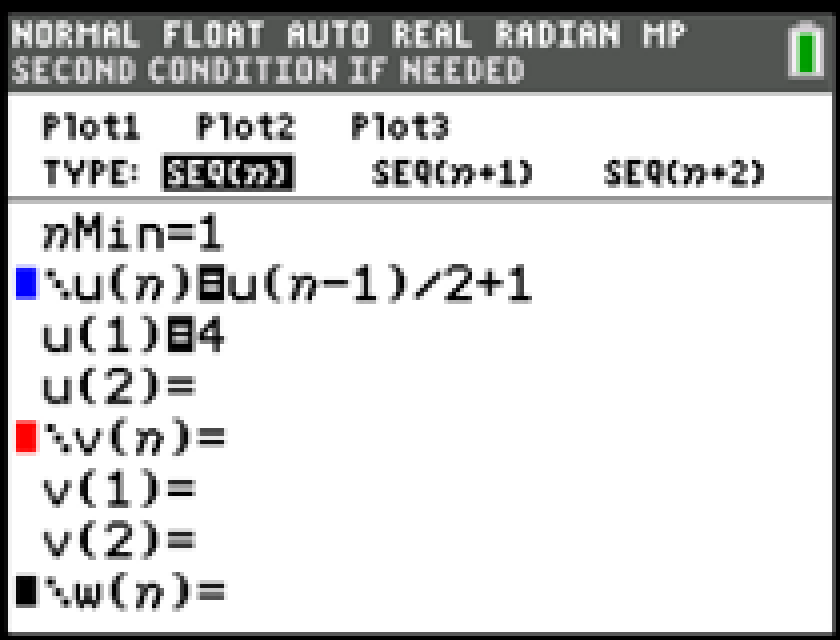
\includegraphics[width=0.48\linewidth]{gc/ex61_yeditor.png}\hfill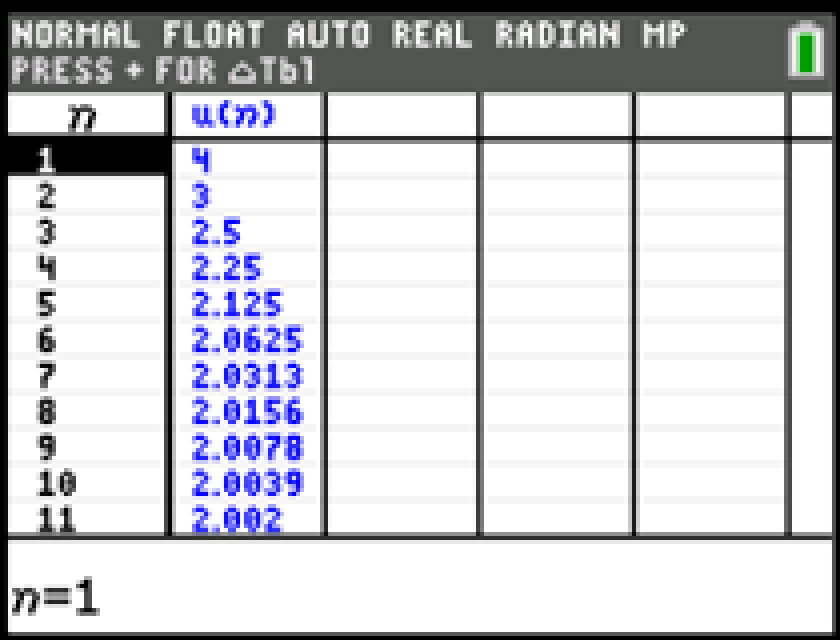
\includegraphics[width=0.48\linewidth]{gc/ex61_table.png}\par}
\end{minipage}\par\smallskip
\exlab
\cdisp{\fhlm{u_{r}}&=\fhlm{2u_{r-1}}+1,\quad u_1=1}
\exlab
\noindent\begin{minipage}[c]{0.58\textwidth}
\cdisp{\fhlm{u_{n}}&=\fhlm{u_{n-1}+2u_{n-2}},\quad u_1=1,\quad u_2=1\\&1,\ 1,\ 3,\ 5,\ 11,\ 21,\ 43,\ \dots}
\end{minipage}\hfill\begin{minipage}[c]{0.38\textwidth}\centering
\par\smallskip{\centering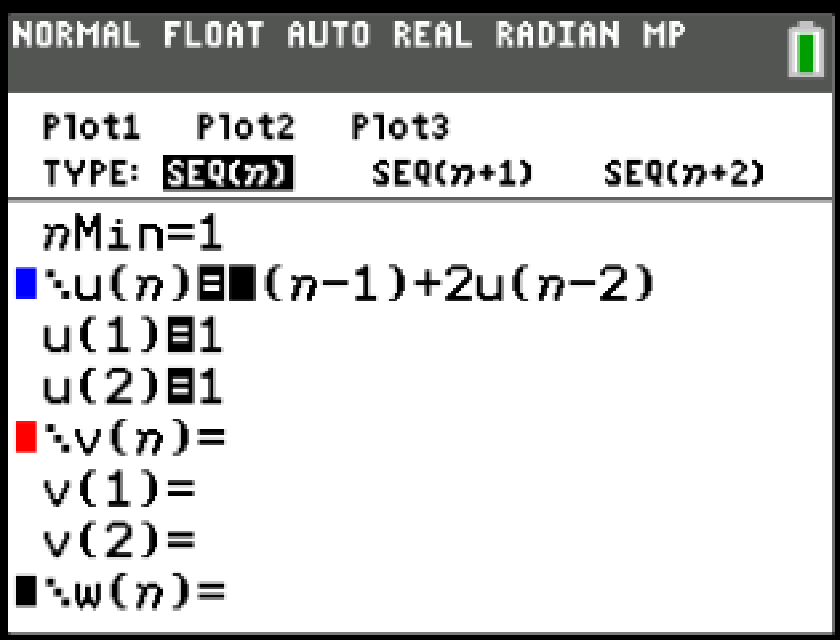
\includegraphics[width=0.48\linewidth]{gc/ex63_yeditor.png}\hfill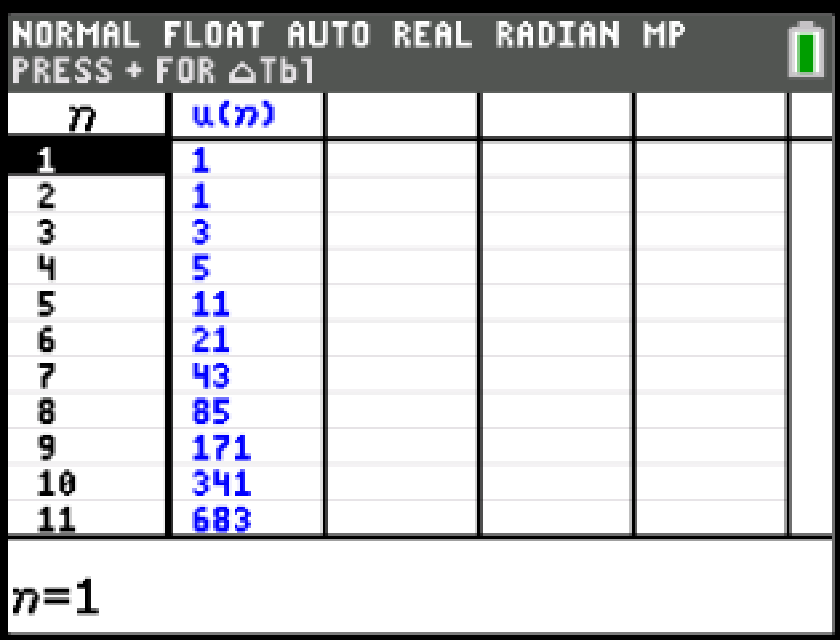
\includegraphics[width=0.48\linewidth]{gc/ex63_table.png}\par}
\end{minipage}\par\smallskip
\noindent\begin{minipage}[t]{0.4\textwidth}
\exlab {\small(GP)}
\cdisp{\fhlm{u_{n}}&=\fhlm{ru_{n-1}},\quad u_1=a\\&a,\ ar,\ ar^{2},\ \dots}
\end{minipage}\hfill\begin{minipage}[t]{0.56\textwidth}
\exlab {\small(AP)}\par
\cdisp{\fhlm{u_{n}}&=\fhlm{u_{n-1}}+d,\quad u_1=a\\&a,\ a+d,\ a+2d,\ \dots}
(However, this is not unique.)
\cdisp{\fhlm{u_{n}-2u_{n-1}+u_{n-2}}&=0,\quad u_1=a,\quad u_2=a+d}
\end{minipage}\par
\subsection{Limit of a Sequence}
\cdisp{\text{As }r\to\infty,\ u_r=\frac1r&\to0\quad\text{or}\quad\lim_{r\to\infty}\left(u_r\right)=\lim_{r\to\infty}\left(\frac1r\right)=0\\\text{As }r\to\infty,\ u_r&\to L\quad\text{or}\quad\lim_{r\to\infty}\left(u_r\right)=L\quad\text{(convergent)}}
$u_r\to L\Rightarrow{}$\fhl{$u_{r-1}\to L,\ u_{r-2}\to L$}$,\ \dots$\par
(For recurrence relations: if the sequence is given to be convergent, change all \fhl{$u_n$, $u_{n-1}$, $u_{n-2}$} to $L$ and solve for $L$.)\par
\textbf{Rules} ($\lim u_r$, $\lim v_r$ real):
\cdisp{\lim_{r\to\infty}\left(a\right)&=a\\\lim_{r\to\infty}\left(u_r\pm v_r\right)&=\lim_{r\to\infty}\left(u_r\right)\pm\lim_{r\to\infty}\left(v_r\right)\\\lim_{r\to\infty}\left(u_rv_r\right)&=\lim_{r\to\infty}\left(u_r\right)\times\lim_{r\to\infty}\left(v_r\right)\\\lim_{r\to\infty}\left(\frac{u_r}{v_r}\right)&=\frac{\lim_{r\to\infty}\left(u_r\right)}{\lim_{r\to\infty}\left(v_r\right)},\quad \lim_{r\to\infty}\left(v_r\right)\neq0}
\section{Sigma Notation}
\cdisp{\sum_{r=m}^{n}\mathrm{f}(r)&=\mathrm{f}(m)+\mathrm{f}(m+1)+\cdots+\mathrm{f}(n)\\S_n=\sum_{r=1}^{n}u_r&=u_1+u_2+\cdots+u_n\quad\text{\small\color{gray!70}(By default, $S_n$ starts from $r=1$ unless otherwise stated.)}}
\textbf{Properties:}
\cdisp{\text{no. of terms in }\sum_{r=m}^{n}u_r&:\ n-m+1\\\sum_{r=m}^{n}a&=(n-m+1)a\\\sum_{r=m}^{n}au_r&=a\sum_{r=m}^{n}u_r\\\sum_{r=m}^{n}\left(u_r\pm v_r\right)&=\sum_{r=m}^{n}u_r\pm\sum_{r=m}^{n}v_r\\\sum_{r=m}^{n}u_r&=\sum_{r=1}^{n}u_r-\sum_{r=1}^{m-1}u_r}
\sidenote{(To remember the last three, note that the properties are similar to what you can do in integration.)}\par
\clearpage
\section{Standard Formulas}
\noindent\begin{minipage}[t]{0.48\textwidth}
\topdisplay{\boxed{\sum_{r=1}^{n}r=\frac{n(n+1)}{2}}}
{\color{gray}AP with first term $1$, common difference $1$:
\cdisp{\sum_{r=1}^{n}r&=1+2+\cdots+n\\S_n&=\frac{n}{2}\left[2(1)+(n-1)(1)\right]\\&=\frac{n(n+1)}{2}}}
\end{minipage}\hfill\begin{minipage}[t]{0.48\textwidth}
\topdisplay{\boxed{\sum_{r=1}^{n}a^{r}=\frac{a\left(a^{n}-1\right)}{a-1},\quad a\neq1}}
{\color{gray}GP with first term $a$, common ratio $a$:
\cdisp{\sum_{r=1}^{n}a^{r}&=a+a^{2}+\cdots+a^{n}\\&=\frac{a\left(a^{n}-1\right)}{a-1}}}
\end{minipage}\par
\noindent\begin{minipage}[t]{0.48\textwidth}
\topdisplay{\boxed{\sum_{r=1}^{n}r^{2}=\frac{n(n+1)(2n+1)}{6}}}
\end{minipage}\hfill\begin{minipage}[t]{0.48\textwidth}
\topdisplay{\boxed{\sum_{r=1}^{n}r^{3}=\left[\frac{n(n+1)}{2}\right]^{2}=\frac{n^{2}(n+1)^{2}}{4}}}
\end{minipage}\par
\begin{info}[title=Note]
$\sum r^{2}$ and $\sum r^{3}$ are given in the exam if needed. All four results hold only if $r$ starts from $1$.
\end{info}
\section{Augmented Forms}
\exlab
\cdisp{\sum_{r=1}^{n}\frac{4}{5^{2r+1}}&=4\sum_{r=1}^{n}\frac{1}{5\cdot25^{r}}\\&=\frac45\sum_{r=1}^{n}\left(\frac{1}{25}\right)^{r}\\&=\frac45\cdot\frac{\frac{1}{25}\left[1-\left(\frac{1}{25}\right)^{n}\right]}{1-\frac{1}{25}}\\&=\frac45\cdot\frac{1}{24}\left[1-\left(\frac{1}{25}\right)^{n}\right]\\&=\frac{1}{30}\left(1-\frac{1}{25^{n}}\right)}
\begin{info}[title=Note]
To use the $\sum a^{r}$ formula, the power must be exactly $r$, not $r+1$, not $2r$. Rewrite first.
\end{info}
\clearpage
\section{Substitution}
\cdisp{\sum_{r=m}^{n}\mathrm{f}(r)=\sum_{r=m-k}^{n-k}\mathrm{f}(r+k)\quad\text{(replace $r$ with $r+k$)}}
\exlab
Given $\displaystyle\sum_{r=2}^{n}\frac{1}{r(r+2)}=\frac12\left(\frac56-\frac{1}{n+1}-\frac{1}{n+2}\right)$, find $\displaystyle\sum_{r=2}^{n}\frac{1}{r^{2}-1}$.
\cdisp{\sum_{r=2}^{n}\frac{1}{r^{2}-1}&=\sum_{r=2}^{n}\frac{1}{(r-1)(r+1)}\\&=\sum_{r=1}^{n-1}\frac{1}{r(r+2)}\quad\text{(replace $r$ with $r+1$)}\\&=\sum_{r=1}^{1}\frac{1}{r(r+2)}+\sum_{r=2}^{n-1}\frac{1}{r(r+2)}\\&=\frac13+\frac12\left(\frac56-\frac1n-\frac{1}{n+1}\right)\\&=\frac34-\frac{1}{2n}-\frac{1}{2(n+1)}}
\begin{info}[title=Note]
Substitution only allows \textbf{translation} of $r$ values, e.g.\ replace $r$ with $\ldots$, $r-2$, $r-1$, $r+1$, $r+2$, $\ldots$\par
Scaling is not allowed. E.g.\ replacing $r$ with $2r$ is wrong. List out the terms to see why.
\end{info}
\clearpage
\section{Convergence}
\exlab
Given $u_n=\dfrac{1}{n(n+1)}$ and $S_n=\displaystyle\sum_{r=1}^{n}u_r=1-\frac{1}{n+1}$.\par\smallskip
{\centering\renewcommand{\arraystretch}{1.3}\begin{tabular}{|p{0.36\textwidth}|p{0.56\textwidth}|}\hline
\textbf{Convergence of $u_n$:} let $n\to\infty$ in $u_n$. & \textbf{Convergence of $S_n$:} let $n\to\infty$ in $S_n$.\\\hline
$\displaystyle\begin{aligned}u_n&=\frac{1}{n(n+1)}\\\text{As }n\to\infty,\ u_n&\to0\end{aligned}$ &
$\displaystyle\begin{aligned}S_n&=\sum_{r=1}^{n}\frac{1}{r(r+1)}\\&=1-\frac{1}{n+1}\\\text{As }n\to\infty,\ S_n&\to1\ \text{(finite)}\\\therefore\ \text{the series converges},\ S_\infty&=1\end{aligned}$\\\hline
\end{tabular}\par}
\begin{info}[title=Note]
(1) $u_n\to0$ is not strong enough evidence that $S_n$ converges, e.g.\ $1+\frac12+\frac13+\frac14+\cdots=\infty$.\par
(2) However, if $S_n$ converges, then $u_n$ \textbf{must} converge to $0$.
\end{info}
\section{Finding \texorpdfstring{$u_n$}{u\_n} or \texorpdfstring{$S_n$}{S\_n} from Each Other}
\subsection{Finding \texorpdfstring{$u_n$}{u\_n} from \texorpdfstring{$S_n$}{S\_n}}
\cdisp{u_n&=S_n-S_{n-1},\quad u_1=S_1}
\exlab
\cdisp{S_n&=n^{2}+2n\\u_n&=S_n-S_{n-1}\\&=\left(n^{2}+2n\right)-\left[(n-1)^{2}+2(n-1)\right]\\&=2n+1}
\fhl{\sidenote{Check: $u_1=S_1=3=2(1)+1$, as $u_n=S_n-S_{n-1}$ only holds for $n\geq2$.}}\par
\subsection{Finding \texorpdfstring{$S_n$}{S\_n} from \texorpdfstring{$u_n$}{u\_n}}
\exlab
\cdisp{u_r&=3r^{2}+r\\S_n&=\sum_{r=1}^{n}\left(3r^{2}+r\right)\\&=3\cdot\frac{n(n+1)(2n+1)}{6}+\frac{n(n+1)}{2}\fhlmi{=\cdots}}
\clearpage
\inchap{Arithmetic and Geometric Progressions}
An \textbf{arithmetic progression (AP)} is a sequence with a common difference $d$, e.g.\ $2,\ 5,\ 8,\ 11,\ \dots$\par
A \textbf{geometric progression (GP)} is a sequence with a common ratio $r$, e.g.\ $3,\ 6,\ 12,\ 24,\ \dots$\par
$u_n$: the $n$th term,\qquad $S_n$: the sum of the first term up to the $n$th term.\par\smallskip
{\centering\renewcommand{\arraystretch}{1.5}\begin{tabular}{|p{0.15\textwidth}|p{0.36\textwidth}|p{0.36\textwidth}|}\hline
 & \textbf{AP} & \textbf{GP}\\\hline
Property & common difference $d$ & common ratio $r$\\\hline
Example & $2,\ 5,\ 8,\ 11,\ \dots$\quad($d=3$) & $3,\ 6,\ 12,\ 24,\ \dots$\quad($r=2$)\\\hline
$u_n$ & $\displaystyle u_n=a+(n-1)d$ & $\displaystyle u_n=ar^{n-1}$\\\hline
$S_n$ & $\displaystyle S_n=\frac n2\left[2a+(n-1)d\right]$\par\smallskip $\displaystyle S_n=\frac n2\left(a+l\right)$ & $\displaystyle S_n=\frac{a\left(1-r^{n}\right)}{1-r}=\frac{a\left(r^{n}-1\right)}{r-1}$,\ $r\neq1$\\\hline
$S_\infty$ & not convergent \fhl{\sidenote{(unless $a=d=0$)}} & $\displaystyle S_\infty=\frac{a}{1-r}$, only if $|r|<1$\\\hline
Proving & $u_{n+1}-u_n=d$ (constant)\par\smallskip
{\color{red}$u_3-u_2=k_1$, $u_2-u_1=k_2$\par $k_1\neq k_2$ $\therefore$ not an AP} &
$\dfrac{u_{n+1}}{u_n}=r$ (constant)\par\smallskip
{\color{red}$\dfrac{u_3}{u_2}=k_1$, $\dfrac{u_2}{u_1}=k_2$\par $k_1\neq k_2$ $\therefore$ not a GP}\\\hline
\end{tabular}\par}
\smallskip
{\color{gray!70}However, to prove that something IS an AP, you have to do it in terms of $n$. You cannot compare $u_1$, $u_2$ and $u_3$ in the same way that we prove that something is not an AP.}\par
\textbf{Note:}\quad AP: $u_2,\ u_4,\ u_6,\ \dots$ is an AP (common difference $2d$),\qquad GP: $u_2,\ u_4,\ u_6,\ \dots$ is a GP (common ratio $r^{2}$).\par
\begin{info}[title=Important Note]
Remember that you can use a GC table whenever needed, especially when the variable you are solving for is an integer. It is very common in this chapter because a lot of the time you are solving for $n\in\mathbb{Z}^{+}$.
\end{info}
\section{Summing}
\exlab
AP: first term $9$, common difference $2$. Sum of the 20th to 50th terms inclusive:
\cdisp{S_{50}-S_{19}&=\frac{50}{2}\left[2(9)+49(2)\right]-\frac{19}{2}\left[2(9)+18(2)\right]\\&=2900-513\\&=2387}
\section{Common Questions}
\subsection{Comparing AP and GP terms}
\exlab {\small[TMJC 2025 Prelim P1 Q4]}\par
An arithmetic series has first term $a$ and common difference $d$, where $a$ and $d$ are non-zero real constants. A convergent geometric series has first term $b$ and common ratio $r$, where $b>0$ and $r$ is a non-zero real constant. The sum of the first $n$ terms of the geometric series is denoted by $S$.\par
It is given that the 7th, 10th and 11th terms of the arithmetic series are equal to the 3rd, 6th and 10th terms of the geometric series respectively.
\cdisp{a+6d&=br^{2}\quad--\ (1)\\a+9d&=br^{5}\quad--\ (2)\\a+10d&=br^{9}\quad--\ (3)}
\subsection{Bank Questions}
\begin{info}[title=Important Note]
\fhl{Many} bank questions will come in the form $u_{n+1}=pu_n+q$, where $p$ and $q$ are constants.
\end{info}
\medskip
\exlab {\small[TJC 2025 Prelim P1 Q7]}\par
\fhl{Janice deposits} \$100 at the start of every month into a bank account that earns 0.3\% interest per month, with interest calculated and added into the account at the end of each month.\par
Find the amount that Janice will have in her savings account at the end of $N$ months.\par\medskip
{\small\renewcommand{\arraystretch}{1.3}\begin{tabular}{|l|l|l|}\hline
$n$th mth&Amount at start of month (\$)&Amount at end of month (\$)\\\hline
1 Jan26&$100$&$100(1.003)$\\\hline
2&$\begin{aligned}[t]&100+100(1.003)\\&=100(1+1.003)\end{aligned}$&$\begin{aligned}[t]&100(1+1.003)(1.003)\\&=100\left(1.003+1.003^{2}\right)\end{aligned}$\\\hline
3&$\begin{aligned}[t]&100+100\left(1.003+1.003^{2}\right)\\&=100\left(1+1.003+1.003^{2}\right)\end{aligned}$&$\begin{aligned}[t]&100\left(1+1.003+1.003^{2}\right)(1.003)\\&=100\left(1.003+1.003^{2}+1.003^{3}\right)\end{aligned}$\\\hline
$\vdots$&$\vdots$&$\vdots$\\\hline
$N$&&$\begin{aligned}[t]&100\left(1.003+1.003^{2}+\dots+1.003^{N}\right)\\&=\frac{100(1.003)\left(1.003^{N}-1\right)}{1.003-1}\end{aligned}$\\\hline
\end{tabular}}\par\medskip
\needspace{14\baselineskip}
\subsection{Contextual Questions}
For general contextual questions, it is important to determine whether the question is asking for $u_n$ or $S_n$.\par
\exlab {\small[RVHS 2025 Prelim P2 Q4]}\par
The dosage of medicine given to a patient needs to be carefully managed in order to achieve the desired result.
\begin{enumerate}[label=(\alph*)]
\item To give the patient time to adapt to a particular medicine, the dosage is slowly increased over time. The patient is initially given a dosage of 0.75 units. The dosage is increased by 0.5 units each day until a total of at least 10 units of medicine has been taken. Find the least number of days it takes to achieve this, and the dosage on that day.\hfill[4]
\item The doctor prescribed a new medication to another patient. After $n$ days, the total dosage of the new medicine administered to the patient is given by $\dfrac{3}{20}\left(\dfrac{5^{n}-4^{n}}{5^{n-1}}\right)$ units.
\begin{enumerate}[label=(\roman*)]
\item Show that the increase in dosage of the new medicine administered per day follows a geometric progression.\hfill[3]
\item Find the total dosage of the new medicine administered to the patient after a long period of treatment.\hfill[2]
\end{enumerate}
\item Doctors can manage the medication so that the daily dosage of medicine increases as an arithmetic progression. Explain in context why the arithmetic progression is not a preferred model for the dosage of medication.\hfill[1]
\end{enumerate}
\clearpage
\inchap{Differentiation}
\section{Basic Differentials}
{\centering\renewcommand{\arraystretch}{1.9}\begin{tabular}{|c|c|}\hline
$y$ & $\dfrac{\mathrm{d}y}{\mathrm{d}x}$\\\hline
$x^{n}$ & $nx^{n-1}$\\\hline
$\sin x$ & $\cos x$\\\hline
$\cos x$ & $-\sin x$\\\hline
$\tan x$ & $\sec^{2}x$\\\hline
$\log_{b}x$ & $\dfrac{1}{x\ln b}$,\ $b$ constant\\\hline
$\mathrm{e}^{\mathrm{f}(x)}$ & $\mathrm{f}'(x)\,\mathrm{e}^{\mathrm{f}(x)}$\\\hline
$a^{\mathrm{f}(x)}$ & $\mathrm{f}'(x)\,a^{\mathrm{f}(x)}\ln a$,\ $a$ constant\\\hline
$\mathrm{p}(x)\,\mathrm{q}(x)$ & $\mathrm{p}'(x)\,\mathrm{q}(x)+\mathrm{p}(x)\,\mathrm{q}'(x)$\\\hline
$\dfrac{\mathrm{p}(x)}{\mathrm{q}(x)}$ & $\dfrac{\mathrm{p}'(x)\,\mathrm{q}(x)-\mathrm{p}(x)\,\mathrm{q}'(x)}{\left[\mathrm{q}(x)\right]^{2}}$\\\hline
\end{tabular}\qquad
\begin{tabular}{|c|c|}\hline
$y$ & $\dfrac{\mathrm{d}y}{\mathrm{d}x}$\\\hline
$\sin^{-1}x$ & $\dfrac{1}{\sqrt{1-x^{2}}}$\\\hline
$\cos^{-1}x$ & $-\dfrac{1}{\sqrt{1-x^{2}}}$\\\hline
$\tan^{-1}x$ & $\dfrac{1}{1+x^{2}}$\\\hline
$\sec x$ & $\sec x\tan x$\\\hline
$\operatorname{cosec}x$ & $-\operatorname{cosec}x\cot x$\\\hline
{\color{blue}$\cot x$} & {\color{blue}$-\operatorname{cosec}^{2}x$}\\\hline
\end{tabular}\par}
\begin{info}[title=Important Note]
Remember to multiply by the differential when you are differentiating. Bracket, not divide.
\end{info}
\needspace{22\baselineskip}
\subsection{Implicit Differentiation}
\exlab
\cdisp{x^{3}y+1+\ln y&=\cos(xy)}
Differentiate both sides with respect to $x$:
\cdisp{3x^{2}y+x^{3}\frac{\mathrm{d}y}{\mathrm{d}x}+0+\frac{1}{y}\frac{\mathrm{d}y}{\mathrm{d}x}&=-\sin(xy)\left(y+x\frac{\mathrm{d}y}{\mathrm{d}x}\right)\\
3x^{2}y+x^{3}\frac{\mathrm{d}y}{\mathrm{d}x}+\frac{1}{y}\frac{\mathrm{d}y}{\mathrm{d}x}&=-y\sin(xy)-x\sin(xy)\frac{\mathrm{d}y}{\mathrm{d}x}\\
x^{3}\frac{\mathrm{d}y}{\mathrm{d}x}+\frac{1}{y}\frac{\mathrm{d}y}{\mathrm{d}x}+x\sin(xy)\frac{\mathrm{d}y}{\mathrm{d}x}&=-y\sin(xy)-3x^{2}y\\
\frac{\mathrm{d}y}{\mathrm{d}x}\left(x^{3}+\frac{1}{y}+x\sin(xy)\right)&=-y\left(\sin(xy)+3x^{2}\right)\\
\frac{\mathrm{d}y}{\mathrm{d}x}\left(\frac{x^{3}y+1+xy\sin(xy)}{y}\right)&=-y\left(\sin(xy)+3x^{2}\right)\\
\therefore\ \frac{\mathrm{d}y}{\mathrm{d}x}&=-\frac{y^{2}\left(\sin(xy)+3x^{2}\right)}{x^{3}y+1+xy\sin(xy)}}
\subsection{Parametric Differentiation}
\cdisp{\frac{\mathrm{d}y}{\mathrm{d}x}=\frac{\mathrm{d}y}{\mathrm{d}t}\times\frac{\mathrm{d}t}{\mathrm{d}x}}
\exlab
\cdisp{x&=t+\sin t,\quad y=1-\cos t\\
\frac{\mathrm{d}x}{\mathrm{d}t}&=1+\cos t,\quad\frac{\mathrm{d}y}{\mathrm{d}t}=\sin t\\
\frac{\mathrm{d}t}{\mathrm{d}x}&=\dfrac{1}{\dfrac{\mathrm{d}x}{\mathrm{d}t}}=\frac{1}{1+\cos t}\\
\frac{\mathrm{d}y}{\mathrm{d}x}&=\frac{\mathrm{d}y}{\mathrm{d}t}\times\frac{\mathrm{d}t}{\mathrm{d}x}\\
&=\frac{\sin t}{1+\cos t}\\
&=\frac{2\sin\frac{t}{2}\cos\frac{t}{2}}{2\cos^{2}\frac{t}{2}}\\
&=\frac{\sin\frac{t}{2}}{\cos\frac{t}{2}}\\
\therefore\ \frac{\mathrm{d}y}{\mathrm{d}x}&=\tan\frac{t}{2}}
\clearpage
\inchap{Applications of Differentiation}
\section{Tangents \& Normals}
A tangent can be diagonal, vertical or horizontal.\par
Gradient of tangent = value of $\dfrac{\mathrm{d}y}{\mathrm{d}x}$.\par
Gradient of normal:
\cdisp{m_{\text{tangent}}\times m_{\text{normal}}&=-1}
Equation of tangent: $y=mx+c$. To find $c$, substitute any point on the tangent.\par\smallskip
\noindent\fhlp{\small\textbf{Horizontal and vertical tangents} at $(x_0,y_0)$:\par\smallskip
\renewcommand{\arraystretch}{1.5}\begin{tabular}{@{}l@{\ \ }l@{}}
Horizontal: & $\dfrac{\mathrm{d}y}{\mathrm{d}x}=0$,\ \ tangent $y=y_0$,\ \ normal $x=x_0$\\
Vertical: & $\dfrac{\mathrm{d}x}{\mathrm{d}y}=0$ \ ($\dfrac{\mathrm{d}y}{\mathrm{d}x}$ undefined),\ \ tangent $x=x_0$,\ \ normal $y=y_0$
\end{tabular}}\par
\subsection{Standard Curves}
\exlab
Find the equation of the tangent to $y=x^{2}-3x+5$ at $x=2$.
\cdisp{\text{When }x=2,\quad y&=2^{2}-3(2)+5=3\\
\frac{\mathrm{d}y}{\mathrm{d}x}&=2x-3\\
\text{When }x=2,\quad\frac{\mathrm{d}y}{\mathrm{d}x}&=2(2)-3=1\\
y&=x+c\\
3&=2+c\\
c&=1\\
\therefore\ y&=x+1}
\subsection{Implicit Curves}
\exlab {\small[EJC 2025 Prelim P2 Q1(b)]}\par
The curve $C$ has equation $x^{3}+y^{3}-3xy=k$, where $k$ is a positive constant. There are two points on $C$ where the tangents are parallel to the $y$-axis. Given that $k=3$, find the exact $y$-coordinates of these two points.
\cdisp{\frac{\mathrm{d}y}{\mathrm{d}x}&=\frac{y-x^{2}}{y^{2}-x}}
Tangent parallel to $y$-axis $\Rightarrow\dfrac{\mathrm{d}y}{\mathrm{d}x}$ undefined:
\cdisp{y^{2}-x&=0\\
x&=y^{2}\\
y^{6}-2y^{3}-3&=0\\
\left(y^{3}-3\right)\left(y^{3}+1\right)&=0\\
\therefore\ y=3^{\frac{1}{3}}\quad&\text{or}\quad y=-1}
\subsection{Parametric Curves}
\exlab {\small[MI 2025 Prelim P2 Q2(i)]}\par
A curve $C$ has parametric equations $x=\sqrt{t}$, $y=t^{2}+4$, where $0\leqslant t\leqslant16$. Find the equation of the tangent to $C$ at the point $P$ with parameter $p$.
\cdisp{\frac{\mathrm{d}x}{\mathrm{d}t}&=\frac{1}{2\sqrt{t}},\quad\frac{\mathrm{d}y}{\mathrm{d}t}=2t\\
\frac{\mathrm{d}y}{\mathrm{d}x}&=\frac{2t}{\frac{1}{2\sqrt{t}}}=4t^{\frac{3}{2}}\\
y-\left(p^{2}+4\right)&=4p^{\frac{3}{2}}\left(x-\sqrt{p}\right)\\
\therefore\ y&=4p^{\frac{3}{2}}x-3p^{2}+4}
\section{Max/Min}
\begin{itemize}
\item To find the stationary value of $y$, solve $\dfrac{\mathrm{d}y}{\mathrm{d}x}=0$.
\item Then, to find/prove its nature, perform the first/second derivative test.
\end{itemize}
\begin{info}[title=Important Note]
In many questions, you may be asked to prove the equation of the quantity you are trying to maximise. It's important to not spend too long on it if you can't prove it. Just continue with the rest of the question to differentiate and solve $\dfrac{\mathrm{d}y}{\mathrm{d}x}=0$.
\end{info}
\par\medskip
{\small\renewcommand{\arraystretch}{1.3}\begin{longtable}{|c|p{3.9cm}|>{\raggedright\arraybackslash}p{2.7cm}|>{\raggedright\arraybackslash}p{4.0cm}|>{\raggedright\arraybackslash}p{2.9cm}|}\hline
Index&Diagram&Info&Equation&Comments\\\hline\endhead
1&{\footnotesize[TJC 2025 Prelim P2 Q4]}\par {\centering\adjustbox{max width=\linewidth,max height=3.6cm}{\figTJCfa\hspace{4mm}\raisebox{0.6cm}{\figTJCfb}}\par}&Constant: radius $a$\newline Variables: angle $\theta$&Prove that\newline $\displaystyle V^{2}=\dfrac{a^{6}}{576\pi^{4}}\theta^{4}\left(4\pi^{2}-\theta^{2}\right)$&Take advantage of the constant slant height and major arc length $AB$.\\\hline
2&{\footnotesize[DHS 2025 Prelim P1 Q11]}\par {\centering\adjustbox{max width=\linewidth,max height=3.6cm}{\figDHSa}\par}&Constant: budget \$$k$\newline Variables: $r$&Prove that\newline $\displaystyle V=\dfrac{k}{20}r-\dfrac{10}{3}\pi r^{3}$&Use the constant budget $k$ to eliminate $L$.\\\hline
3&{\footnotesize[TJC 2024 Promo Q12]}\par {\centering\adjustbox{max width=\linewidth,max height=3.6cm}{\figTJCsph}\par}&Constant: sphere radius $R$\newline Variables: $h$&Prove that\newline $\displaystyle r^{2}=\dfrac{h^{2}R^{2}}{h^{2}-2hR}$&Take advantage of the constant sphere radius $R$, and similar triangles. Pythagoras theorem is useful here too.\\\hline
4&{\footnotesize[CJC 2024 Promo Q10]}\par {\centering\adjustbox{max width=\linewidth,max height=3.6cm}{\figCJC}\par}&Constant: volume $20\pi$ cm$^{3}$\newline Variables: $r$&Prove that\newline $\displaystyle A\dfrac{\mathrm{d}A}{\mathrm{d}r}=\pi^{2}\left(2r^{3}-\dfrac{3600}{r^{3}}\right)$&Use the constant volume to eliminate $h$. For rate of change questions, use similar triangles.\\\hline
5&{\footnotesize[EJC 2018 Promo Q7]}\par {\centering\adjustbox{max width=\linewidth,max height=3.6cm}{\figEJC}\par}&Constant: slant edge $R$\newline Variables: $x$&Prove that\newline $\displaystyle 9V^{2}=\pi^{2}x^{4}\left(R^{2}-x^{2}\right)$&Use the constant $R$ to eliminate $h$.\\\hline
6&{\footnotesize[TMJC 2024 Prelim P1 Q2]}\par {\centering\adjustbox{max width=\linewidth,max height=3.6cm}{\figTMJC}\par}&Constant: sphere radius $k$\newline \fhl{Variables: $h$, $r$}&---&Use the constant radius of sphere $k$ and Pythagoras theorem is useful here too.\\\hline
\end{longtable}}
\section{Rate of Change}
\cdisp{\frac{\mathrm{d}y}{\mathrm{d}t}=\frac{\mathrm{d}y}{\mathrm{d}x}\times\frac{\mathrm{d}x}{\mathrm{d}t}}
\textbf{Step 1:} Identify what information is given.\par
\textbf{Step 2:} Form the missing equation if necessary and differentiate it.\par
\exlab
Given $y=x^{2}-4x+1$ and $\dfrac{\mathrm{d}x}{\mathrm{d}t}=3$, find the rate of change of $y$ when $x=5$.
\cdisp{\frac{\mathrm{d}y}{\mathrm{d}x}&=2x-4\\
\text{When }x=5,\quad\frac{\mathrm{d}y}{\mathrm{d}x}&=2(5)-4=6\\
\frac{\mathrm{d}y}{\mathrm{d}t}&=\frac{\mathrm{d}y}{\mathrm{d}x}\times\frac{\mathrm{d}x}{\mathrm{d}t}\\
&=6\times3\\
\therefore\ \frac{\mathrm{d}y}{\mathrm{d}t}&=18}

\clearpage
\inchap{Power Series}
\section{Standard Formulae (MF27)}
\begin{align*}
(1+x)^{n}&=1+nx+\frac{n(n-1)}{2!}x^{2}+\dots+\frac{n(n-1)\cdots(n-r+1)}{r!}x^{r}+\dots\quad(|x|<1)\tag{1}\\[1ex]
\mathrm{e}^{x}&=1+x+\frac{x^{2}}{2!}+\dots+\frac{x^{r}}{r!}+\dots\quad(\text{all }x)\tag{2}\\[1ex]
\sin x&=x-\frac{x^{3}}{3!}+\frac{x^{5}}{5!}-\dots+\frac{(-1)^{r}x^{2r+1}}{(2r+1)!}+\dots\quad(\text{all }x)\tag{3}\\[1ex]
\cos x&=1-\frac{x^{2}}{2!}+\frac{x^{4}}{4!}-\dots+\frac{(-1)^{r}x^{2r}}{(2r)!}+\dots\quad(\text{all }x)\tag{4}\\[1ex]
\ln(1+x)&=x-\frac{x^{2}}{2}+\frac{x^{3}}{3}-\dots+\frac{(-1)^{r+1}x^{r}}{r}+\dots\quad(-1<x\leqslant1)\tag{5}
\end{align*}
\begin{info}[title=Important Note]
For equations (1) and (5), the constant must be 1.
\end{info}
\cautionbox{Any substituted expressions of $x$ cannot have \fhl{``$+$ constant inside} hl{\sidenote{(more precisely, the substituted term must tend to $0$)}}.
\cdisp{\text{\ding{55}}\quad\mathrm{e}^{1+x+x^{2}+\cdots}&=1+\left(1+x+x^{2}+\cdots\right)+\frac{\left(1+x+x^{2}+\cdots\right)^{2}}{2!}+\cdots\\[1ex]
\text{\ding{51}}\quad\mathrm{e}^{1+x+x^{2}+\cdots}&=\mathrm{e}^{1}\cdot\mathrm{e}^{x+x^{2}+\cdots}\\
&=\mathrm{e}\left[1+\left(x+x^{2}+\cdots\right)+\frac{\left(x+x^{2}+\cdots\right)^{2}}{2!}+\cdots\right]}}
\section{Maclaurin Series}
\cdisp{\mathrm{f}(x)&=\mathrm{f}(0)+x\,\mathrm{f}'(0)+\frac{x^{2}}{2!}\mathrm{f}''(0)+\dots+\frac{x^{r}}{r!}\mathrm{f}^{(r)}(0)+\dots}
Conditions for existence: for all $n\in\mathbb{Z}^{+}\cup\{0\}$, $\mathrm{f}^{(n)}$ is differentiable and $\mathrm{f}^{(n)}(0)$ is defined.
\newpage
\section{Small Angle Approximations}
When $\theta$ is sufficiently small, $\theta^{3}$ and above can be ignored.
\cdisp{\sin\theta&\approx\theta\\\cos\theta&\approx1-\frac{\theta^{2}}{2}\\\tan\theta&\approx\theta}
\exlab
\cdisp{\sin2\theta&\approx2\theta}
\exlab
\cdisp{\cos3\theta&\approx1-\frac{(3\theta)^{2}}{2}\\&=1-\frac{9\theta^{2}}{2}}
\exlab
\cdisp{\sec\theta&=\frac{1}{\cos\theta}\\&\approx\left(1-\frac{\theta^{2}}{2}\right)^{-1}\\&\approx1+\frac{\theta^{2}}{2}}
\exlab
$\sin\left(\frac{\pi}{4}+\theta\right)\not\approx\frac{\pi}{4}+\theta$
\cdisp{\sin\left(\frac{\pi}{4}+\theta\right)&=\sin\frac{\pi}{4}\cos\theta+\cos\frac{\pi}{4}\sin\theta\\&=\frac{1}{\sqrt{2}}\left(\cos\theta+\sin\theta\right)\\&\approx\frac{1}{\sqrt{2}}\left(1-\frac{\theta^{2}}{2}+\theta\right)\\\therefore\ \sin\left(\frac{\pi}{4}+\theta\right)&\approx\frac{1}{\sqrt{2}}\left(1+\theta-\frac{\theta^{2}}{2}\right)}
\section{General Approximations}
\begin{itemize}
\item Values of $x$ closer to 0 give better approximations as higher powers of $x$ are less significant.
\item Values of $x$ outside the range of validity give an inaccurate approximation.
\end{itemize}
%% CHAPTER 11 INTEGRATION -- rebuilt from Maximus's "Integration Techniques" summary PDF
\providecommand{\cautionbox}[2][CAUTION]{\begin{info}[title={#1}]#2\end{info}}
\providecommand{\ddx}{\,\mathrm{d}x}
\clearpage
\inchap{Integration}
\section{Basic Integrals}
{\renewcommand{\arraystretch}{2.1}\centering\begin{tabular}{|>{\centering\arraybackslash}m{6.6cm}|>{\centering\arraybackslash}m{7.6cm}|}\hline
\textbf{Basic}&\textbf{General form} (let $a$, $b$, $k$ be constants)\\\hline
$\displaystyle \int x^{n}\ddx=\frac{x^{n+1}}{n+1}+c,\quad n\neq-1$&$\displaystyle \int(ax+b)^{n}\ddx=\frac{(ax+b)^{n+1}}{a(n+1)}+c,\quad n\neq-1$\\\hline
$\displaystyle \int\frac1x\ddx=\ln|x|+c$&$\displaystyle \int\frac{1}{ax+b}\ddx=\frac1a\ln|ax+b|+c$\\\hline
$\displaystyle \int\mathrm{e}^{x}\ddx=\mathrm{e}^{x}+c$&$\displaystyle \int\mathrm{e}^{kx}\ddx=\frac1k\mathrm{e}^{kx}+c$\\\hline
$\displaystyle \int\sin x\ddx=-\cos x+c$&$\displaystyle \int\sin kx\ddx=-\frac1k\cos kx+c$\\\hline
$\displaystyle \int\cos x\ddx=\sin x+c$&$\displaystyle \int\cos kx\ddx=\frac1k\sin kx+c$\\\hline
$\displaystyle \int\sec^{2}x\ddx=\tan x+c$&$\displaystyle \int\sec^{2}kx\ddx=\frac1k\tan kx+c$\\\hline
\end{tabular}\par}
\section{$\mathrm{f}'(x)$ Formulas}
\cdisp{\int\mathrm{f}'(x)\left[\mathrm{f}(x)\right]^{n}\ddx&=\frac{\left[\mathrm{f}(x)\right]^{n+1}}{n+1}+c,\qquad n\neq-1\\
\int\frac{\mathrm{f}'(x)}{\mathrm{f}(x)}\ddx&=\ln|\mathrm{f}(x)|+c\\
\int\mathrm{f}'(x)\,\mathrm{e}^{\mathrm{f}(x)}\ddx&=\mathrm{e}^{\mathrm{f}(x)}+c}
\section{New Trigonometric Integrals}
\begin{itemize}
\item To find $\displaystyle\int\tan x\ddx$, $\displaystyle\int\sec x\ddx$, $\displaystyle\int\operatorname{cosec}x\ddx$, $\displaystyle\int\cot x\ddx$ --- see the \textbf{MF27}.
\item To find $\displaystyle\int\sin^{2}x\ddx$ or $\displaystyle\int\cos^{2}x\ddx$, use the \textbf{double angle formula} for $\cos2\theta$.\newline
To find $\displaystyle\int\tan^{2}x\ddx$, use the identity $\tan^{2}x=\sec^{2}x-1$.
\item The differentiation formulas for $\sec x$ and $\operatorname{cosec}x$ in the MF27 can also be used as \textbf{integration} formulas. In particular, the missing formula yields
\cdisp{\int\operatorname{cosec}^{2}x\ddx=-\cot x+c.}
\end{itemize}
\section{Standard MF27 Formulas}
{\renewcommand{\arraystretch}{2.4}\centering\begin{tabular}{|>{\centering\arraybackslash}m{6.6cm}|>{\centering\arraybackslash}m{7.6cm}|}\hline
\textbf{Standard}&\textbf{General form}\\\hline
$\displaystyle \int\frac{1}{a^{2}+x^{2}}\ddx=\frac1a\tan^{-1}\frac xa+c$&$\displaystyle \int\frac{\mathrm{f}'(x)}{a^{2}+\left[\mathrm{f}(x)\right]^{2}}\ddx=\frac1a\tan^{-1}\frac{\mathrm{f}(x)}{a}+c$\\\hline
$\displaystyle \int\frac{1}{\sqrt{a^{2}-x^{2}}}\ddx=\sin^{-1}\frac xa+c$&$\displaystyle \int\frac{\mathrm{f}'(x)}{\sqrt{a^{2}-\left[\mathrm{f}(x)\right]^{2}}}\ddx=\sin^{-1}\frac{\mathrm{f}(x)}{a}+c$\\\hline
$\displaystyle \int\frac{1}{x^{2}-a^{2}}\ddx=\frac{1}{2a}\ln\left|\frac{x-a}{x+a}\right|+c$&$\displaystyle \int\frac{\mathrm{f}'(x)}{\left[\mathrm{f}(x)\right]^{2}-a^{2}}\ddx=\frac{1}{2a}\ln\left|\frac{\mathrm{f}(x)-a}{\mathrm{f}(x)+a}\right|+c$\\\hline
$\displaystyle \int\frac{1}{a^{2}-x^{2}}\ddx=\frac{1}{2a}\ln\left|\frac{a+x}{a-x}\right|+c$&$\displaystyle \int\frac{\mathrm{f}'(x)}{a^{2}-\left[\mathrm{f}(x)\right]^{2}}\ddx=\frac{1}{2a}\ln\left|\frac{a+\mathrm{f}(x)}{a-\mathrm{f}(x)}\right|+c$\\\hline
\end{tabular}\par}
\cautionbox[IMPORTANT]{$a$ must be a (positive) \textbf{constant}.}
\begin{info}[title=Important Remark]
When using these formulas, it is \textbf{VERY COMMON} to have to complete the square first.
\end{info}
\begin{info}[title=Remark]
These formulas are commonly used together with $\mathrm{f}'(x)$ formulas to integrate \textbf{rational functions}.
\end{info}
\exlab
\cdisp{\int\frac{4x}{\sqrt{4x-x^{2}}}\ddx&=\int\frac{-2(-2x+4)+8}{\sqrt{4x-x^{2}}}\ddx\\
&=-2\int(-2x+4)\left(4x-x^{2}\right)^{-\frac12}\ddx+8\int\frac{1}{\sqrt{4-(x-2)^{2}}}\ddx\\
&=-2\cdot\frac{\left(4x-x^{2}\right)^{\frac12}}{\left(\frac12\right)}+8\sin^{-1}\frac{x-2}{2}+c\\
&=-4\sqrt{4x-x^{2}}+8\sin^{-1}\frac{x-2}{2}+c}
\clearpage
\section{Integration by Parts (IKID)}
\begin{center}\textbf{\color{red}I}\textbf{ntegrate}\quad\textbf{\color{red}K}\textbf{eep}\quad\textbf{\color{red}I}\textbf{ntegrate}\quad\textbf{\color{red}D}\textbf{ifferentiate}\end{center}
\cdisp{IK-\int ID\ddx}
\exlab
\cdisp{\int\underbrace{x}_{\text{K/D}}\,\underbrace{\mathrm{e}^{x}}_{\text{I}}\ddx=\underbrace{\mathrm{e}^{x}}_{\text{I}}\,\underbrace{x}_{\text{K}}-\int\underbrace{\mathrm{e}^{x}}_{\text{I}}\,\underbrace{1}_{\text{D}}\ddx}
\begin{itemize}
\item It is possible to make the \textbf{wrong choice} of which expression to integrate. In such scenarios, the $\int ID\ddx$ will look \textit{worse} than the original problem.
\item It is common to have to \textbf{IKID twice}. Consider this approach if you are unable to continue.
\end{itemize}
\cautionbox[IMPORTANT]{Integration by parts is often used as the \textbf{last resort}, i.e.\ please consider \textbf{ALL OTHER INTEGRATION TECHNIQUES} first.}
\textbf{Common tricks}
\begin{itemize}
\item \textbf{IKID by multiplying by 1.}
\cdisp{\int\ln x\ddx=\int1\cdot\ln x\ddx=\dots}
\item \textbf{Non-obvious splitting.}
\cdisp{\int x^{3}\mathrm{e}^{x^{2}}\ddx=\int x^{2}\cdot x\mathrm{e}^{x^{2}}\ddx=\dots}
Here, we can integrate $x\mathrm{e}^{x^{2}}$ using the $\int\mathrm{f}'(x)\mathrm{e}^{\mathrm{f}(x)}\ddx$ formula.
\item \textbf{Loop method.}
\cdisp{\int\mathrm{e}^{x}\cos x\ddx&=\mathrm{e}^{x}\cos x+\int\mathrm{e}^{x}\sin x\ddx\\
&=\mathrm{e}^{x}\cos x+\mathrm{e}^{x}\sin x-\int\mathrm{e}^{x}\cos x\ddx}
Therefore,
\cdisp{2\int\mathrm{e}^{x}\cos x\ddx&=\mathrm{e}^{x}\cos x+\mathrm{e}^{x}\sin x+c\\
\int\mathrm{e}^{x}\cos x\ddx&=\frac12\left(\mathrm{e}^{x}\cos x+\mathrm{e}^{x}\sin x\right)+c}
\end{itemize}
\clearpage
\section{Integration by Substitution}
Given $\displaystyle\int\mathrm{f}(x)\ddx$ and a substitution $u=\dots$, apply:\par
\textbf{Step 1:} Substitute $u$ into $\mathrm{f}(x)$.\par
\textbf{Step 2:} Find $\dfrac{\mathrm{d}x}{\mathrm{d}u}$, and substitute it into the integral.\par
\textbf{Step 3:} \textit{(Only for definite integrals)} Substitute the limits of integration from $x$ values to $u$ values.\par
{\setlength{\columnseprule}{0.4pt}\begin{multicols}{2}
{\centering\textbf{Indefinite Integral}\par}
\exlab
\fhlp{Using the substitution $x=\sin u$, where $0\leqslant u\leqslant\frac{\pi}{2}$, find $\displaystyle\int\sqrt{1-x^{2}}\ddx$.}\par
\cdisp{&\int\sqrt{1-x^{2}}\ddx,\qquad x=\sin u\\
={}&\int\underbrace{\sqrt{1-\sin^{2}u}}_{\text{Step 1}}\,\underbrace{\cos u\,\mathrm{d}u}_{\text{Step 2}}\\
={}&\int\sqrt{\cos^{2}u}\,\cos u\,\mathrm{d}u\\
={}&\int\cos^{2}u\,\mathrm{d}u\\
={}&\frac12\int\left(1+\cos2u\right)\mathrm{d}u\\
={}&\frac12\left(u+\frac12\sin2u\right)+c\\
={}&\frac12u+\frac12\sin u\cos u+c\\
={}&\frac12\sin^{-1}x+\frac12x\sqrt{1-x^{2}}+c}
\begin{center}\fbox{\begin{minipage}{5.4cm}\centering\vspace{1mm}\begin{tikzpicture}[scale=1.6]
\draw[thick] (0,0)--(1.6,0)--(1.6,1)--cycle;
\draw (1.45,0)--(1.45,0.15)--(1.6,0.15);
\node[above left] at (0.8,0.5){$1$}; \node[right] at (1.6,0.5){$x$}; \node[below] at (0.8,0){$\sqrt{1-x^{2}}$};
\draw (0.35,0) arc(0:32:0.35); \node at (0.5,0.12){\scriptsize$u$};
\end{tikzpicture}\par
\cdisp{\sin u&=x\\\cos u&=\sqrt{1-x^{2}}}\end{minipage}}\end{center}
\columnbreak
{\centering\textbf{Definite Integral}\par}
\exlab
\fhlp{Using the substitution $x=\sin u$, find the exact value of $\displaystyle\int_{0}^{\frac12}\sqrt{1-x^{2}}\ddx$.}\par
\cdisp{&\int_{0}^{\frac12}\sqrt{1-x^{2}}\ddx,\qquad x=\sin u\\
x=0\ &\Rightarrow\ u=0\\
x=\frac12\ &\Rightarrow\ u=\frac{\pi}{6}\\
\int_{0}^{\frac12}\sqrt{1-x^{2}}\ddx&=\int_{0}^{\frac{\pi}{6}}\sqrt{1-\sin^{2}u}\,\cos u\,\mathrm{d}u\\
&=\int_{0}^{\frac{\pi}{6}}\cos^{2}u\,\mathrm{d}u\\
&=\frac12\int_{0}^{\frac{\pi}{6}}\left(1+\cos2u\right)\mathrm{d}u\\
&=\frac12\left[u+\frac12\sin2u\right]_{0}^{\frac{\pi}{6}}\\
&=\frac12\left[\left(\frac{\pi}{6}+\frac12\sin\frac{\pi}{3}\right)-\left(0+\frac12\sin0\right)\right]\\
&=\frac12\left(\frac{\pi}{6}+\frac{\sqrt3}{4}\right)\\
&=\frac{\pi}{12}+\frac{\sqrt3}{8}}
\end{multicols}}
\begin{info}[title=Remark]
Remember to sub the final answer back to be in terms of $x$, unless it's a \textbf{definite integral}.
\end{info}

%% CHAPTER 12 DEFINITE INTEGRALS -- dictated by Maximus (25 Oct 2026); diagrams adapted from h2-math-notes/aoi/notes (figstyles sketch/curve/solX/solY)
\providecommand{\cautionbox}[2][CAUTION]{\begin{info}[title={#1}]#2\end{info}}
\providecommand{\ddx}{\,\mathrm{d}x}\providecommand{\ddy}{\,\mathrm{d}y}
\pgfplotsset{dimini/.style={sketch,width=3.7cm,height=3.1cm,every node/.append style={font=\scriptsize}}}
\newcommand{\rsum}[1]{% #1 = 0 left, 1 right
\begin{tikzpicture}[x=0.95cm,y=0.75cm,font=\scriptsize]
\def\f(##1){0.5+0.18*(##1)*(##1)}
\foreach \k in {0,1,2}{\pgfmathsetmacro\xl{0.8+0.5*\k}\pgfmathsetmacro\xr{\xl+0.5}\pgfmathsetmacro\xs{#1==0?\xl:\xr}
 \fill[blue!22,draw=blue!60!black,thin] (\xl,0) rectangle (\xr,{0.5+0.18*\xs*\xs});}
\foreach \k in {0,1}{\pgfmathsetmacro\xl{3.1+0.5*\k}\pgfmathsetmacro\xr{\xl+0.5}\pgfmathsetmacro\xs{#1==0?\xl:\xr}
 \fill[blue!22,draw=blue!60!black,thin] (\xl,0) rectangle (\xr,{0.5+0.18*\xs*\xs});}
\node at (2.7,0.55) {$\cdots$};
\draw[->,thick] (-0.2,0)--(4.4,0) node[right]{$x$}; \draw[->,thick] (0,-0.2)--(0,4.0) node[above]{$y$};
\draw[blue,semithick,domain=0.5:4.3,samples=60] plot (\x,{0.5+0.18*\x*\x}) node[right]{$y=\mathrm{f}(x)$};
\node[below] at (0.8,0){$a$}; \node[below] at (1.3,0){$a\!+\!h$}; \node[below] at (1.8,-0.3){$a\!+\!2h$};
\node[below] at (2.7,0){$\cdots$}; \node[below] at (4.1,0){$b$};
\end{tikzpicture}}
\newcommand{\vsolo}[1]{\adjustbox{totalheight=1.9cm,max width=6.6cm}{#1}}\newcommand{\vpair}[2]{\adjustbox{totalheight=1.9cm,max width=6.6cm}{#1\;\raisebox{0.15ex}{\Large$-$}\;#2}}
\newcommand{\cellfig}[2]{\begin{minipage}[t]{\linewidth}\centering\vspace{0pt}#1\\[-0.5mm]{\footnotesize$\displaystyle #2$}\vspace{1mm}\end{minipage}}
\clearpage
\inchap{Definite Integrals}
\cdisp{\int_{a}^{b}\mathrm{f}(x)\ddx=\Big[\mathrm{F}(x)\Big]_{a}^{b}=\mathrm{F}(b)-\mathrm{F}(a)}
\section{Area as a Limit of a Sum}
{\renewcommand{\arraystretch}{1.3}\centering\begin{tabular}{|>{\centering\arraybackslash}m{7.6cm}|>{\centering\arraybackslash}m{7.6cm}|}\hline
\textbf{Left-hand sum}&\textbf{Right-hand sum}\\\hline
\rsum{0}&\rsum{1}\\\hline
$\displaystyle\lim_{n\to\infty}\sum_{r=0}^{n-1}\frac{b-a}{n}\,\mathrm{f}\left(a+\frac{r(b-a)}{n}\right)=\int_{a}^{b}\mathrm{f}(x)\ddx$&$\displaystyle\lim_{n\to\infty}\sum_{r=1}^{n}\frac{b-a}{n}\,\mathrm{f}\left(a+\frac{r(b-a)}{n}\right)=\int_{a}^{b}\mathrm{f}(x)\ddx$\\[3mm]\hline
Increasing $\mathrm{f}(x)\Rightarrow$ underestimate\newline Decreasing $\mathrm{f}(x)\Rightarrow$ overestimate&Increasing $\mathrm{f}(x)\Rightarrow$ overestimate\newline Decreasing $\mathrm{f}(x)\Rightarrow$ underestimate\\\hline
\end{tabular}\par}
\medskip
%% ---------------- dx / dy table
\newcommand{\gX}[2]{\begin{tikzpicture}\begin{axis}[dimini,xmin=-0.3,xmax=4.3,#1]#2\end{axis}\end{tikzpicture}}
{\renewcommand{\arraystretch}{1.15}\setlength{\tabcolsep}{3pt}\centering\begin{longtable}{|>{\raggedright\arraybackslash}m{2.3cm}|>{\centering\arraybackslash}m{7.15cm}|>{\centering\arraybackslash}m{7.15cm}|}\hline
\textbf{Index}&$\boldsymbol{\mathrm{d}x}$&$\boldsymbol{\mathrm{d}y}$\\\hline\endhead
Area under curve&
\cellfig{\gX{ymin=-0.3,ymax=3}{\fill[blue!22] (axis cs:1,0)--plot[domain=1:3.4,samples=30](axis cs:\x,{1+0.15*\x*\x})--(axis cs:3.4,0)--cycle;\addplot[curve,domain=0.4:3.9]{1+0.15*x*x};\node[below] at (axis cs:1,0){$a$};\node[below] at (axis cs:3.4,0){$b$};}}{\int_{a}^{b}y\ddx}&
\cellfig{\gX{ymin=-0.3,ymax=3.4}{\fill[blue!22] (axis cs:0,0.8)--plot[domain=0.8:2.8,samples=30](axis cs:{1+0.25*\x*\x},\x)--(axis cs:0,2.8)--cycle;\addplot[curve,variable=t,domain=0.4:3.2]({1+0.25*t*t},{t});\node[left] at (axis cs:0,0.8){$c$};\node[left] at (axis cs:0,2.8){$d$};}}{\int_{c}^{d}x\ddy}\\\hline
Negative areas&
\cellfig{\gX{ymin=-3,ymax=0.5}{\fill[blue!22] (axis cs:1,0)--plot[domain=1:3.4,samples=30](axis cs:\x,{-1-0.15*\x*\x})--(axis cs:3.4,0)--cycle;\addplot[curve,domain=0.4:3.9]{-1-0.15*x*x};\node[above] at (axis cs:1,0){$a$};\node[above] at (axis cs:3.4,0){$b$};}}{-\int_{a}^{b}y\ddx}&
\cellfig{\gX{xmin=-4.3,xmax=0.4,ymin=-0.3,ymax=3.4}{\fill[blue!22] (axis cs:0,0.8)--plot[domain=0.8:2.8,samples=30](axis cs:{-1-0.25*\x*\x},\x)--(axis cs:0,2.8)--cycle;\addplot[curve,variable=t,domain=0.4:3.2]({-1-0.25*t*t},{t});\node[right] at (axis cs:0,0.8){$c$};\node[right] at (axis cs:0,2.8){$d$};}}{-\int_{c}^{d}x\ddy}\\\hline
Areas between two graphs&
\cellfig{\gX{ymin=-0.3,ymax=3.4,width=3.1cm}{\fill[blue!22] plot[domain=1:3.4,samples=30](axis cs:\x,{2.2+0.1*\x})--plot[domain=3.4:1,samples=30](axis cs:\x,{0.4+0.12*(\x-2)^2})--cycle;\addplot[curve,domain=0.5:3.9]{2.2+0.1*x};\addplot[line2,red!75!black,domain=0.5:3.9,samples=40]{0.4+0.12*(x-2)^2};\draw[dashed,thin](axis cs:1,0)--(axis cs:1,2.3);\draw[dashed,thin](axis cs:3.4,0)--(axis cs:3.4,2.54);\node[below] at (axis cs:1,0){$a$};\node[below] at (axis cs:3.4,0){$b$};}\,%
\gX{ymin=-1.8,ymax=2,width=3.1cm}{\fill[blue!22] plot[domain=1:3.4,samples=30](axis cs:\x,{1.2+0.1*\x})--plot[domain=3.4:1,samples=30](axis cs:\x,{-1.2+0.15*(\x-2)^2})--cycle;\addplot[curve,domain=0.5:3.9]{1.2+0.1*x};\addplot[red!75!black,semithick,domain=0.5:3.9,samples=40]{-1.2+0.15*(x-2)^2};\node[above] at (axis cs:1,0){$a$};\node[above] at (axis cs:3.6,0){$b$};}\,%
\gX{ymin=-3.4,ymax=0.4,width=3.1cm}{\fill[blue!22] plot[domain=1:3.4,samples=30](axis cs:\x,{-0.5-0.1*\x})--plot[domain=3.4:1,samples=30](axis cs:\x,{-2.6+0.12*(\x-2)^2})--cycle;\addplot[curve,domain=0.5:3.9]{-0.5-0.1*x};\addplot[red!75!black,semithick,domain=0.5:3.9,samples=40]{-2.6+0.12*(x-2)^2};\node[above] at (axis cs:1,0){$a$};\node[above] at (axis cs:3.4,0){$b$};}}%
{\text{All 3 cases: }\int_{a}^{b}\left(y_{1}-y_{2}\right)\ddx}&
\cellfig{\gX{xmin=-0.3,xmax=3.4,ymin=-0.3,ymax=4.3,width=3.1cm}{\fill[blue!22] plot[domain=1:3.4,samples=30](axis cs:{2.2+0.1*\x},\x)--plot[domain=3.4:1,samples=30](axis cs:{0.4+0.12*(\x-2)^2},\x)--cycle;\addplot[curve,variable=t,domain=0.5:3.9]({2.2+0.1*t},{t});\addplot[red!75!black,semithick,variable=t,domain=0.5:3.9,samples=40]({0.4+0.12*(t-2)^2},{t});\node[left] at (axis cs:0,1){$c$};\node[left] at (axis cs:0,3.4){$d$};}\,%
\gX{xmin=-1.8,xmax=2,ymin=-0.3,ymax=4.3,width=3.1cm}{\fill[blue!22] plot[domain=1:3.4,samples=30](axis cs:{1.2+0.1*\x},\x)--plot[domain=3.4:1,samples=30](axis cs:{-1.2+0.15*(\x-2)^2},\x)--cycle;\addplot[curve,variable=t,domain=0.5:3.9]({1.2+0.1*t},{t});\addplot[red!75!black,semithick,variable=t,domain=0.5:3.9,samples=40]({-1.2+0.15*(t-2)^2},{t});\node[right] at (axis cs:0,1){$c$};\node[right] at (axis cs:0,3.6){$d$};}\,%
\gX{xmin=-3.4,xmax=0.4,ymin=-0.3,ymax=4.3,width=3.1cm}{\fill[blue!22] plot[domain=1:3.4,samples=30](axis cs:{-0.5-0.1*\x},\x)--plot[domain=3.4:1,samples=30](axis cs:{-2.6+0.12*(\x-2)^2},\x)--cycle;\addplot[curve,variable=t,domain=0.5:3.9]({-0.5-0.1*t},{t});\addplot[red!75!black,semithick,variable=t,domain=0.5:3.9,samples=40]({-2.6+0.12*(t-2)^2},{t});\node[right] at (axis cs:0,1){$c$};\node[right] at (axis cs:0,3.4){$d$};}}%
{\text{All 3 cases: }\int_{c}^{d}\left(x_{1}-x_{2}\right)\ddy}\\
&{\scriptsize $y_1$ (blue) above $y_2$ (red)}&{\scriptsize $x_1$ (blue) right of $x_2$ (red)}\\\hline
Volume rotated about axis&
\cellfig{\gX{ymin=-0.3,ymax=3}{\fill[blue!22] (axis cs:1,0)--plot[domain=1:3.4,samples=30](axis cs:\x,{1+0.15*\x*\x})--(axis cs:3.4,0)--cycle;\addplot[curve,domain=0.4:3.9]{1+0.15*x*x};\node[below] at (axis cs:1,0){$a$};\node[below] at (axis cs:3.4,0){$b$};}\\[1mm]\vsolo{\solX[0.9]{1+0.15*x*x}{1}{3.4}{1.15}{2.73}{4}{3.2}{blue!70!black}}}{\text{About the $x$-axis: }\pi\int_{a}^{b}y^{2}\ddx}&
\cellfig{\gX{ymin=-0.3,ymax=3.4}{\fill[blue!22] (axis cs:0,0.8)--plot[domain=0.8:2.8,samples=30](axis cs:{1+0.25*\x*\x},\x)--(axis cs:0,2.8)--cycle;\addplot[curve,variable=t,domain=0.4:3.2]({1+0.25*t*t},{t});\node[left] at (axis cs:0,0.8){$c$};\node[left] at (axis cs:0,2.8){$d$};}\\[1mm]\vsolo{\solY{1+0.25*x*x}{0.8}{2.8}{1.16}{2.96}{3.4}{3.4}{blue!70!black}}}{\text{About the $y$-axis: }\pi\int_{c}^{d}x^{2}\ddy}\\\hline
Volume generated by region between two curves&
\cellfig{\gX{ymin=-0.3,ymax=3.4}{\fill[blue!22] plot[domain=1:3.4,samples=30](axis cs:\x,{2.2+0.1*\x})--plot[domain=3.4:1,samples=30](axis cs:\x,{0.4+0.12*(\x-2)^2})--cycle;\addplot[curve,domain=0.5:3.9]{2.2+0.1*x};\addplot[red!75!black,semithick,domain=0.5:3.9,samples=40]{0.4+0.12*(x-2)^2};\node[below] at (axis cs:1,0){$a$};\node[below] at (axis cs:3.4,0){$b$};}\\[1mm]\vpair{\solX[0.9]{2.2+0.1*x}{1}{3.4}{2.3}{2.54}{4}{3}{blue!70!black}}{\solX[0.9]{0.4+0.12*(x-2)^2}{1}{3.4}{0.52}{0.63}{4}{3}{red!75!black}}}{\pi\int_{a}^{b}\left(y_{1}^{2}-y_{2}^{2}\right)\ddx}&
\cellfig{\gX{xmin=-0.3,xmax=3.4,ymin=-0.3,ymax=4.3}{\fill[blue!22] plot[domain=1:3.4,samples=30](axis cs:{2.2+0.1*\x},\x)--plot[domain=3.4:1,samples=30](axis cs:{0.4+0.12*(\x-2)^2},\x)--cycle;\addplot[curve,variable=t,domain=0.5:3.9]({2.2+0.1*t},{t});\addplot[red!75!black,semithick,variable=t,domain=0.5:3.9,samples=40]({0.4+0.12*(t-2)^2},{t});\node[left] at (axis cs:0,1){$c$};\node[left] at (axis cs:0,3.4){$d$};}\\[1mm]\vpair{\solY{2.2+0.1*x}{1}{3.4}{2.3}{2.54}{3.2}{4}{blue!70!black}}{\solY{0.4+0.12*(x-2)^2}{1}{3.4}{0.52}{0.63}{3.2}{4}{red!75!black}}}{\pi\int_{c}^{d}\left(x_{1}^{2}-x_{2}^{2}\right)\ddy}\\\hline
\end{longtable}\par}
When finding \textbf{area}, we generally have the choice to integrate via $\mathrm{d}x$ or $\mathrm{d}y$. Some considerations:
\begin{itemize}
\item $\mathrm{d}x$ or $\mathrm{d}y$ easier to integrate
\item do we need to add or subtract regular shapes like rectangles
\item is it even possible to make $x$ (or $y$) the subject?
\end{itemize}
For \textbf{volume}, we cannot choose which variable to integrate with respect to.
\begin{itemize}
\item Region rotated about the $x$-axis: $\displaystyle\pi\int_{a}^{b}y^{2}\ddx$
\item Region rotated about the $y$-axis: $\displaystyle\pi\int_{c}^{d}x^{2}\ddy$
\end{itemize}
\begin{info}[title={Important Note: dealing with conics}]
When making $y$ the subject, the sign of the square root indicates which half of the conic is being considered.\par\smallskip
\textbf{Example}\quad $(x-1)^{2}+(y-2)^{2}=9$\par
{\renewcommand{\arraystretch}{1.1}\centering\begin{tabular}{>{\centering\arraybackslash}m{5cm}>{\centering\arraybackslash}m{3.2cm}}
$\displaystyle y=2+\sqrt{9-(x-1)^{2}}$&\begin{tikzpicture}[scale=0.32]\draw[->](-2.6,0)--(4.8,0) node[right]{\tiny$x$};\draw[->](0,-1.6)--(0,5.8) node[above]{\tiny$y$};\draw[gray!60,dashed](1,2) circle(3);\draw[blue,ultra thick](1,2)++(0:3) arc(0:180:3);\fill(1,2) circle(2pt);\end{tikzpicture}\\
$\displaystyle y=2-\sqrt{9-(x-1)^{2}}$&\begin{tikzpicture}[scale=0.32]\draw[->](-2.6,0)--(4.8,0) node[right]{\tiny$x$};\draw[->](0,-1.6)--(0,5.8) node[above]{\tiny$y$};\draw[gray!60,dashed](1,2) circle(3);\draw[blue,ultra thick](1,2)++(180:3) arc(180:360:3);\fill(1,2) circle(2pt);\end{tikzpicture}\\
$\displaystyle x=1+\sqrt{9-(y-2)^{2}}$&\begin{tikzpicture}[scale=0.32]\draw[->](-2.6,0)--(4.8,0) node[right]{\tiny$x$};\draw[->](0,-1.6)--(0,5.8) node[above]{\tiny$y$};\draw[gray!60,dashed](1,2) circle(3);\draw[blue,ultra thick](1,2)++(-90:3) arc(-90:90:3);\fill(1,2) circle(2pt);\end{tikzpicture}\\
$\displaystyle x=1-\sqrt{9-(y-2)^{2}}$&\begin{tikzpicture}[scale=0.32]\draw[->](-2.6,0)--(4.8,0) node[right]{\tiny$x$};\draw[->](0,-1.6)--(0,5.8) node[above]{\tiny$y$};\draw[gray!60,dashed](1,2) circle(3);\draw[blue,ultra thick](1,2)++(90:3) arc(90:270:3);\fill(1,2) circle(2pt);\end{tikzpicture}
\end{tabular}\par}
Note: this concept can be used for any conic. That is, circles, ellipses, hyperbolas, parabolas.
\end{info}
\textbf{Notes on volume}
\begin{itemize}
\item ``Rotate $\pi$ radians about \dots'' does not usually mean the formula has to be divided by 2. It just means that rotating only $180^{\circ}$ is sufficient to generate the full solid. The volume remains as $\pi\int_a^b y^2\ddx$.
\item To find the volume of rotating regions ``below'' the axis, there is no need to put a negative sign in front:
\cdisp{\textcolor{red}{\text{\ding{55}}}\quad-\pi\int_{a}^{b}y^{2}\ddx\qquad\qquad\textcolor{green!45!black}{\text{\ding{51}}}\quad\pi\int_{a}^{b}y^{2}\ddx}
\item Common mistake for volume between two graphs:
\cdisp{\textcolor{red}{\text{\ding{55}}}\quad\pi\int_{a}^{b}\left(y_{1}-y_{2}\right)^{2}\ddx\qquad\qquad\textcolor{green!45!black}{\text{\ding{51}}}\quad\pi\int_{a}^{b}\left(y_{1}^{2}-y_{2}^{2}\right)\ddx}
\end{itemize}
\begin{info}[title=Important Note]
Take note if the question asks for exact or not. If they did not, please evaluate the integral using GC rather than integration by hand.
\end{info}
\begin{info}[title=Remark]
If an integral seems very difficult/impossible to integrate, then check if the question wants exact form OR check if you have integrated something similar in earlier parts.
\end{info}
\subsection*{\fhl{12.1.1}\quad Regular Shapes in Area and Volume}\addcontentsline{toc}{subsection}{\protect\numberline{12.1.1}Regular Shapes in Area and Volume}
Sometimes we may encounter familiar shapes like squares, rectangles, triangles, trapeziums, cones, and cylinders. It will be useful to use the formulas for these shapes/solids for efficiency.
\begin{multicols}{3}
\centering
\begin{tikzpicture}[scale=0.8]\draw[thick,fill=blue!15](0,0) rectangle (1.8,1.8);\node[below] at (0.9,0){$a$};\node[left] at (0,0.9){$a$};\end{tikzpicture}\\Square: $\text{Area}=a^{2}$\par\medskip
\begin{tikzpicture}[scale=0.8]\draw[thick,fill=blue!15](0,0) rectangle (2.8,1.6);\node[below] at (1.4,0){$l$};\node[left] at (0,0.8){$b$};\end{tikzpicture}\\Rectangle: $\text{Area}=lb$\par\medskip
\columnbreak
\begin{tikzpicture}[scale=0.8]\draw[thick,fill=blue!15](0,0)--(2.8,0)--(1.0,1.8)--cycle;\draw[dashed](1.0,1.8)--(1.0,0);\draw(1.0,0.2)--(1.2,0.2)--(1.2,0);\node[below] at (1.4,0){$b$};\node[right] at (1.0,0.9){$h$};\end{tikzpicture}\\Triangle: $\text{Area}=\frac12bh$\par\medskip
\begin{tikzpicture}[scale=0.8]\draw[thick,fill=blue!15](0,0)--(3,0)--(2.3,1.6)--(0.6,1.6)--cycle;\draw[dashed](0.6,1.6)--(0.6,0);\node[below] at (1.5,0){$b$};\node[above] at (1.45,1.6){$a$};\node[left] at (0.6,0.8){$h$};\end{tikzpicture}\\Trapezium: $\text{Area}=\frac12(a+b)h$\par\medskip
\columnbreak
\begin{tikzpicture}[scale=0.8]\fill[blue!15](-1,0)--(0,2.2)--(1,0) arc(0:-180:1 and 0.3);\draw[thick](-1,0)--(0,2.2)--(1,0);\draw[thick](1,0) arc(0:-180:1 and 0.3);\draw[dashed](1,0) arc(0:180:1 and 0.3);\draw[dashed](0,0)--(0,2.2);\draw[dashed](0,0)--(1,0);\node[right] at (0,1.1){$h$};\node[above] at (0.5,0){$r$};\end{tikzpicture}\\Cone: $\text{Volume}=\frac13\pi r^{2}h$\par\medskip
\begin{tikzpicture}[scale=0.8]\fill[blue!15](-1,0)--(-1,1.8) arc(180:360:1 and 0.3)--(1,0) arc(0:-180:1 and 0.3);\draw[thick,fill=blue!8](0,1.8) ellipse(1 and 0.3);\draw[thick](-1,0)--(-1,1.8);\draw[thick](1,0)--(1,1.8);\draw[thick](1,0) arc(0:-180:1 and 0.3);\draw[dashed](1,0) arc(0:180:1 and 0.3);\draw[dashed](0,1.8)--(1,1.8);\node[above] at (0.5,1.8){$r$};\node[right] at (1,0.9){$h$};\end{tikzpicture}\\Cylinder: $\text{Volume}=\pi r^{2}h$
\end{multicols}
\subsection*{\fhl{12.1.2}\quad Integration with Modulus}\addcontentsline{toc}{subsection}{\protect\numberline{12.1.2}Integration with Modulus}
To integrate with modulus, we determine where the function inside the modulus is positive and where it is negative, then split it up.
\exlab
\cdisp{\int_{0}^{\pi}\left|x\sin x\cos x\right|\ddx&=\int_{0}^{\frac{\pi}{2}}{\color{blue}(}x\sin x\cos x{\color{blue})}\ddx+\int_{\frac{\pi}{2}}^{\pi}{\color{red}-(}x\sin x\cos x{\color{red})}\ddx\\
&=\int_{0}^{\frac{\pi}{2}}\frac12x\sin2x\ddx+\int_{\frac{\pi}{2}}^{\pi}{\color{red}-}\frac12x\sin2x\ddx\\
&=\ldots}

%% CHAPTER 13 DIFFERENTIAL EQUATIONS -- dictated by Maximus (26 Oct 2026)
\providecommand{\ddx}{\,\mathrm{d}x}\providecommand{\ddy}{\,\mathrm{d}y}
\newcommand{\DYDX}{\frac{\mathrm{d}y}{\mathrm{d}x}}\newcommand{\DUDX}{\frac{\mathrm{d}u}{\mathrm{d}x}}
\clearpage
\inchap{Differential Equations}
\section{Definition of a Differential Equation}
\begin{theorem}{Differential Equation}
A \textbf{differential equation} is an equation involving a derivative, e.g.\ $\DYDX$, of an unknown function.
\end{theorem}
\section{Solving a Differential Equation}
Solving a differential equation means finding $y$ as a function of $x$ that satisfies the differential equation.
\begin{theorem}{General and Particular Solutions}
\begin{itemize}
\item \textbf{General solution}: a solution containing arbitrary constant(s).
\item \textbf{Particular solution}: a solution where the constant(s) are found from given conditions.
\end{itemize}
\end{theorem}
In this chapter, $C$ and $D$ denote arbitrary constants that are added, and $A$ denotes an arbitrary constant that multiplies.
\subsection{\texorpdfstring{$\DYDX=\mathrm{f}(x)$}{dy/dx = f(x)}}
{\centering{\renewcommand{\arraystretch}{2.2}\begin{tabular}{@{}*{3}{>{$\displaystyle}r<{$}@{}>{$\displaystyle}l<{$}@{\hspace{1.2cm}}}@{}}
\multicolumn{2}{@{}l}{\textbf{Example \stepcounter{exctr}\theexctr}}&\multicolumn{2}{l}{\textbf{Example \stepcounter{exctr}\theexctr}}&\multicolumn{2}{l}{\textbf{Example \stepcounter{exctr}\theexctr}}\\[-2mm]
\DYDX&=3x^{2}&\DYDX&=\mathrm{e}^{2x}&\frac{\mathrm{d}^{2}y}{\mathrm{d}x^{2}}&=6x\\
&\quad\vdots&&\quad\vdots&&\quad\vdots\\
y&=x^{3}+C&y&=\frac12\mathrm{e}^{2x}+C&y&=x^{3}+Cx+D\\
\end{tabular}\par}}
\subsection{Method of Separable Variables}
When a differential equation has ``$y$'' terms, we apply the method of separable variable. Divide the expression in terms of $y$ to the LHS, and keep all $x$ terms on the RHS.
\begin{center}\fbox{\rule[-3mm]{0pt}{10mm}\quad\fhlm{\DYDX=\mathrm{f}(y)\,\mathrm{g}(x)}\quad}\end{center}
{\centering{\renewcommand{\arraystretch}{2.2}\begin{tabular}{@{}*{3}{>{$\displaystyle}r<{$}@{}>{$\displaystyle}l<{$}@{\hspace{1.2cm}}}@{}}
\multicolumn{2}{@{}l}{\textbf{Example \stepcounter{exctr}\theexctr}}&\multicolumn{2}{l}{\textbf{Example \stepcounter{exctr}\theexctr}}&\multicolumn{2}{l}{\textbf{Example \stepcounter{exctr}\theexctr}}\\[-2mm]
\DYDX&=k(30-y)&\DYDX&=ky(1-y)&\DYDX&=xy^{2}+x+y^{2}+1\\
&&&&&=x\left(y^{2}+1\right)+\left(y^{2}+1\right)\\
&&&&&=(x+1)\left(y^{2}+1\right)\\
\frac{1}{30-y}\DYDX&=k&\frac{1}{y(1-y)}\DYDX&=k&\frac{1}{y^{2}+1}\DYDX&=x+1\\
&\quad\vdots&&\quad\vdots&&\quad\vdots\\
\therefore y&=30-A\mathrm{e}^{-kx}&\therefore y&=\frac{1}{1+A\mathrm{e}^{-kx}}&\therefore y&=\tan\left(\frac12x^{2}+x+C\right)\\
\end{tabular}\par}}
\begin{info}[title=Note]
If some values of $x$ and $y$ are given (usually initial values $x=0$, $y=y_{0}$), you should solve for the particular solution.
\end{info}
\begin{info}[title=Note: Sketching graphs of solutions]
\begin{minipage}[c]{0.5\linewidth}
\begin{itemize}
\item \textbf{General solution}: family of curves, i.e.\ many possible different curves.
\item \textbf{Particular solution}: one curve.
\end{itemize}
\end{minipage}\hfill
\begin{minipage}[c]{0.46\linewidth}\centering
\begin{tikzpicture}[x=0.55cm,y=0.06cm,font=\scriptsize]
\draw[->,thick](0,0)--(9,0) node[right]{$x$};\draw[->,thick](0,0)--(0,58) node[above]{$y$};
\draw[dashed](0,30)--(8.8,30) node[right]{$y=30$};
\foreach \A in {-25,-12,12,25}{\draw[blue!60,semithick,domain=0:8.6,samples=50] plot(\x,{30-\A*exp(-0.5*\x)});}
\draw[red!80!black,very thick,domain=0:8.6,samples=50] plot(\x,{30-20*exp(-0.5*\x)});
\node[left] at (0,10){$10$};\node[left] at (0,30){$30$};
\node[red!80!black,align=left,anchor=west] at (2.4,8){particular solution\\$y=30-20\mathrm{e}^{-0.5x}$};
\end{tikzpicture}\\[-1mm]{\scriptsize Family $y=30-A\mathrm{e}^{-0.5x}$}
\end{minipage}
\end{info}
\begin{info}[title=Note]
Most of the time, graphs of solutions to differential equations in H2 Math have horizontal asymptotes. We can find them by letting $x\to\infty$. Alternatively, let $\DYDX=0$ and solve for $y$ if it is a separable variable differential equation. \fhl{Only if $\DYDX$ is a function of $y$ alone.}
\end{info}
\clearpage
\section{Substitution}
Given a differential equation, it may sometimes be impossible to separate the variables. In such cases, a substitution will be given to you (do not come up with your own).
\exlab
{\small (DHS 2025 Prelim P1 Q1)} It is given that $2xy\DYDX=x^{2}-y^{2}$ where $x>0$, $y<0$. Using the substitution $u=\dfrac{y}{x}$, show that the differential equation can be transformed to $\dfrac{2u}{1-3u^{2}}\DUDX=\dfrac{1}{x}$. Hence find the general solution of $y$ in terms of $x$.\par\medskip
\noindent\textbf{Step 1: Differentiate the substitution}
\cdisp{u=\frac{y}{x}\ \Rightarrow\ y&=ux\\{\color{blue}\DYDX}&{\color{blue}{}=\DUDX x+u}\quad\ldots(1)}
\noindent\textbf{Step 2: Substitute the substitution}
\cdisp{2xy\DYDX&=x^{2}-y^{2}\\2x{\color{red}(ux)}{\color{blue}\left(x\DUDX+u\right)}&=x^{2}-{\color{red}(ux)}^{2}\\&\;\;\vdots\\\frac{2u}{1-3u^{2}}\DUDX&=\frac{1}{x}\quad\text{(shown)}\\&\;\;\vdots\\3u^{2}&=1-\frac{A}{x^{3}}\\\left(\frac{y}{x}\right)^{2}&=\frac13\left(1-\frac{A}{x^{3}}\right)\\\therefore y&=-\sqrt{\frac{x^{2}}{3}\left(1-\frac{A}{x^{3}}\right)}=-x\sqrt{\frac13\left(1-\frac{A}{x^{3}}\right)}\quad(\because y<0)}
\begin{caution}
\textbf{\large VERY IMPORTANT NOTE}\par\smallskip
For substitution in differential equations, always remember to substitute the original variables ($x$ and $y$) back into the equation!
\end{caution}
\begin{caution}
\textbf{\large SUPER ULTRA IMPORTANT NOTE}\par\smallskip
The variable in the substitution is \textbf{NOT A CONSTANT} unless otherwise stated!\par\smallskip
Example: $y=ux^{2}$ (product rule: $u$ and $x^{2}$ are both variables)
\cdisp{\textcolor{red}{\text{\ding{55}}}\quad\DYDX=2ux\qquad\qquad\textcolor{green!45!black}{\text{\ding{51}}}\quad\DYDX=x^{2}\DUDX+u(2x)=x^{2}\DUDX+2ux}
\end{caution}

%% CHAPTER 14 COMPLEX NUMBERS -- dictated by Maximus (26 Oct 2026); more to come
\clearpage
\inchap{Complex Numbers}
\section{Cartesian Form}
\begin{definition}{Cartesian form of a complex number}
Every complex number $z\in\mathbb{C}$ can be expressed as $z=x+y\mathrm{i}$, $x,y\in\mathbb{R}$.
\begin{itemize}
\item A complex number $z$ is \textbf{real} if $\operatorname{Im}(z)=0$.
\item A complex number $z$ is \textbf{purely imaginary} if $\operatorname{Re}(z)=0$ \fhl{and $\operatorname{Im}(z)\neq0$}.
\end{itemize}
\end{definition}
\section{Complex Number Arithmetic}
\begin{itemize}
\item \textbf{Addition \& subtraction}: similar to surds.
\item \textbf{Multiplication}: similar to surds.
\item \textbf{Division}: similar to surds, remember to \textit{realise}.
\item \textbf{Square roots} (See Example 14.1)
\end{itemize}
\exlab
Find the values of $\sqrt{3+4\mathrm{i}}$. \fhl{\sidenote{(or, solve for $z^{2}=3+4\mathrm{i}$)}}
\cdisp{(a+b\mathrm{i})^{2}&=3+4\mathrm{i}\\a^{2}-b^{2}+2ab\,\mathrm{i}&=3+4\mathrm{i}}
By comparing real \& imaginary parts,
\cdisp{a^{2}-b^{2}=3,\quad2ab&=4\\&\;\;\vdots\\a=2,\ b=1\text{ or }a=-2,\ b&=-1\\\therefore\sqrt{3+4\mathrm{i}}=2+\mathrm{i}\text{ or }&-2-\mathrm{i}}
\begin{theorem}{Equality of Complex Numbers}
Two complex numbers $z_{1}=a_{1}+b_{1}\mathrm{i}$ and $z_{2}=a_{2}+b_{2}\mathrm{i}$ are equal if and only if their real parts are equal and their imaginary parts are equal.
\[z_{1}=z_{2}\iff a_{1}=a_{2}\text{ and }b_{1}=b_{2}\]
This is basically comparing \textbf{real} and \textbf{imaginary} parts.
\end{theorem}
\section{Simultaneous Equations}
\textbf{Common types:}
\begin{enumerate}
\item Standard $z$, $w$ (no conjugate, no modulus, no square)
\cdisp{2z+w&=2-4\mathrm{i}\\\mathrm{i}z-w&=2\mathrm{i}}
\item With $z^{*}$ and $w$ (or vice versa, or both)
\cdisp{z+2z^{*}+w=6+\mathrm{i}\quad\text{and}\quad\mathrm{i}z-w=3}
\hfill{\small[MI 2025 Prelim P2 Q3(a)]}\par
{\color{gray}If both $z^{*}$ and $w^{*}$ are in the equation, it is still solvable. Consider this example: $z=2+\mathrm{i}w\Rightarrow z^{*}=2-\mathrm{i}w^{*}$}
\item With $z^{2}$ and $w$
\cdisp{\fhlm{z^{2}}-\mathrm{i}w+2&=0\\\fhlm{z}&=w+\mathrm{i}+3}
\hfill{\small[NYJC 2024 Prelim P1 Q1]}\par
{\color{gray}The quadratic formula is useful here; avoid letting $z=a+b\mathrm{i}$ and expanding, though it works.}
\item With $z$ and $|w|$
\cdisp{z+w^{*}+5\mathrm{i}=10\quad\text{and}\quad\left|w\right|^{2}=z+18+\mathrm{i}}
\hfill{\small[CJC 2017 Prelim P2 Q4(a)]}\par
{\color{gray}For $w=a+b\mathrm{i}$, $\left|w\right|=\sqrt{a^{2}+b^{2}}$.}
\end{enumerate}
\begin{info}[title=Note]
Please check your answers using your GC for \textbf{BOTH} equations! The answers are usually quite nice and not ugly numbers.
\end{info}
\clearpage
\section{Polynomials}
\begin{theorem}{Complex Conjugate Root Theorem}
If all the coefficients of a polynomial equation $\mathrm{P}(z)=0$ are real, and $z=\alpha$ is a root, then its conjugate $z=\alpha^{*}$ is also a root.
\end{theorem}

\exlab
{\small[ACJC/2014/I/4]}\par\noindent
\begin{tabular}{@{}p{0.7cm}p{0.88\linewidth}@{}}
(i)&Given that $1+\mathrm{i}$ is a root of the equation $2w^{3}+aw^{2}+bw-2=0$, find the values of the real numbers $a$ and $b$.\hfill[4]\\
(ii)&For these values of $a$ and $b$, solve the equation in part \textbf{\fhl{(i)}}, without the use of a calculator.\hfill[3]
\end{tabular}\par
{\setlength{\columnseprule}{0.4pt}\begin{multicols}{2}
\noindent\textbf{Method 1: Apply CCRT}
\cdisp{w&=1+\mathrm{i}\text{ is a root}\\\therefore w&=1-\mathrm{i}\text{ is a root}\\\left(w-(1+\mathrm{i})\right)\left(w-(1-\mathrm{i})\right)&=(w-1)^{2}-\mathrm{i}^{2}\\&=w^{2}-2w+2\\2w^{3}+aw^{2}+bw-2&=\left(w^{2}-2w+2\right)(Aw+B)\\w^{3}:\quad A&=2\\w^{0}:\quad2B&=-2\\B&=-1\\Aw+B=2w-1&=0\\\therefore w&=\frac12\\w^{2}:\quad a&=B-2A=-5\\w^{1}:\quad b&=2A-2B=6\\\therefore a=-5,\ b&=6\\\therefore w=1+\mathrm{i},\ 1-\mathrm{i},\ &\tfrac12}
\columnbreak
\noindent\textbf{Method 2: Substitute the root}
\cdisp{2(1+\mathrm{i})^{3}+a(1+\mathrm{i})^{2}+b(1+\mathrm{i})-2&=0\\(b-6)+(2a+b+4)\mathrm{i}&=0}
By comparing real \& imaginary parts,
\cdisp{b-6=0,\quad2a+b+4&=0}
\fhlp{\cdisp{\therefore a=-5,\ b&=6\\w&=1+\mathrm{i}\text{ is a root}\\\therefore w&=1-\mathrm{i}\text{ is a root}\\\left(w-(1+\mathrm{i})\right)\left(w-(1-\mathrm{i})\right)&=w^{2}-2w+2\\2w^{3}-5w^{2}+6w-2&=\left(w^{2}-2w+2\right)(Aw+B)\\&\;\;\vdots}
{\centering\color{gray}\small(compare coefficients or long divide)\par}
\cdisp{&\;\;\vdots\\A=2,\ B&=-1\\\therefore w=1+\mathrm{i},\ 1-\mathrm{i},\ &\tfrac12}}
\end{multicols}}
\begin{info}[title=Note]
If you see a really weird question you have never seen before, you can try letting the complex number $=a+b\mathrm{i}$ as a last resort and see where you get with it (unless it becomes unreasonably tedious).
\end{info}
\clearpage
\exlab
{\small[RI Promo/9758/2018/Q11(a)(ii)]} It is given that one of the roots of the equation $z^{3}-(1+4\mathrm{i})z^{2}-(3-9\mathrm{i})z+(14-2\mathrm{i})=0$ is purely imaginary. Find all the roots of the equation, giving your answers in Cartesian form $a+\mathrm{i}b$.\hfill[6]\par
{\color{gray}The coefficients are not all real, so the Complex Conjugate Root Theorem does not apply.}
\cdisp{\text{Let }z&=k\mathrm{i},\ k\in\mathbb{R}\\-k^{3}\mathrm{i}+(1+4\mathrm{i})k^{2}-(3-9\mathrm{i})k\mathrm{i}+14-2\mathrm{i}&=0\\\left(k^{2}-9k+14\right)+\left(-k^{3}+4k^{2}-3k-2\right)\mathrm{i}&=0}
By comparing real \& imaginary parts,
\cdisp{k^{2}-9k+14=0,\quad-k^{3}+4k^{2}-3k-2&=0\\(k-2)(k-7)&=0\\k&=2\text{ or }7\\k=2:\quad-8+16-6-2&=0\\k=7:\quad-343+196-21-2&\neq0\\\therefore k&=2,\quad z=2\mathrm{i}}
\cdisp{{\color{blue}z^{3}-(1+4\mathrm{i})z^{2}-(3-9\mathrm{i})z+(14-2\mathrm{i})}&{\color{blue}=(z-2\mathrm{i})\left(Az^{2}+Bz+C\right)}}
{\color{gray}Here, $A,B,C\in\mathbb{C}$, so we cannot compare real and imaginary parts for an equation involving $A$, $B$ or $C$.}
\cdisp{z^{3}:\quad A&=1\\z^{2}:\quad B-2\mathrm{i}A&=-1-4\mathrm{i}\\B&=-1-2\mathrm{i}\\z^{0}:\quad-2\mathrm{i}C&=14-2\mathrm{i}\\C&=1+7\mathrm{i}\\z^{2}-(1+2\mathrm{i})z+(1+7\mathrm{i})&=0\\z&=\frac{(1+2\mathrm{i})\pm\sqrt{(1+2\mathrm{i})^{2}-4(1+7\mathrm{i})}}{2}\\&=\frac{(1+2\mathrm{i})\pm{\color{red}\sqrt{-7-24\mathrm{i}}}}{2}\quad\text{\color{gray}(use GC here!)}\\&=\frac{(1+2\mathrm{i})\pm(3-4\mathrm{i})}{2}\\\therefore z=2\mathrm{i},\ 2-\mathrm{i},\ &-1+3\mathrm{i}}

{\color{gray}This question does not say ``without using a calculator'', so use your GC to evaluate anything you can, instead of expanding things out manually.}




\clearpage
\section{Argand Diagram}
\subsection{Modulus}
\begin{definition}{Modulus of a Complex Number}
The \textbf{Modulus} of complex number, or absolute value, is defined as:
\[|z|=|a+b\mathrm{i}|=\sqrt{a^{2}+b^{2}}.\]
\end{definition}
It is represented by the distance from the origin, to the coordinate represented by the complex number in an Argand diagram.

\noindent\textbf{Properties of Modulus}\par
Let $z=a+b\mathrm{i}$ and $w=x+y\mathrm{i}$, where $a,b,x,y\in\mathbb{R}$. Then we have the following useful properties.
\begin{center}\begin{tabular}{@{}p{0.46\linewidth}p{0.46\linewidth}@{}}$\bullet$\ $|z|^{2}=a^{2}+b^{2}$. (Obviously)&$\bullet$\ $|z^{*}|=|z|$.\end{tabular}\\[10pt]
\begin{tabular}{@{}p{0.31\linewidth}p{0.31\linewidth}p{0.31\linewidth}@{}}{\color{gray}$\bullet$\ $|zw|=|z||w|$.}&{\color{gray}$\bullet$\ $\left|\dfrac{z}{w}\right|=\dfrac{|z|}{|w|}$.}&{\color{gray}$\bullet$\ $|z^{n}|=|z|^{n}$.}\end{tabular}\end{center}









{\color{gray}You are not required to memorise the last 3 formulas in the 'A' Level syllabus, but may be asked to show them and use it in a question.}

\subsection{Argument}
\begin{definition}{Argument of a Complex Number}
An \textbf{argument} of the complex number $z=x+\mathrm{i}y$, denoted $\arg(z)$, is defined geometrically, as the 2D polar angle $\theta$ from the positive real axis to the vector representing $z$.
\end{definition}
\begin{info}[title=Note]
The argument, $\theta$, of all complex numbers must lie within the range $-\pi<\theta\le\pi$.
\end{info}
Given a complex number, to find its argument,\par
\textbf{Step 1:} find basic angle $\alpha=\tan^{-1}\left|\dfrac{b}{a}\right|$.\par
\textbf{Step 2:} draw a small Argand diagram to figure out which quadrant it is in based on its coordinate. (e.g. $-1+\sqrt3\,\mathrm{i}\iff(-1,\sqrt3)$ is in the 2nd quadrant)
\newcommand{\argd}[3]{\begin{tikzpicture}[scale=0.8,>=stealth]
\draw[->](-1.6,0)--(1.8,0)node[right]{\scriptsize Re};\draw[->](0,-1.6)--(0,1.8)node[above]{\scriptsize Im};
\node[below left]at(0,0){\scriptsize$O$};
\draw[thick](0,0)--(#1,#2);\fill(#1,#2)circle(1.5pt);#3\end{tikzpicture}}
\begin{center}
\renewcommand{\arraystretch}{1.4}\begin{tabular}{|*{4}{>{\centering\arraybackslash}m{\dimexpr0.25\linewidth-2\tabcolsep-1pt\relax}|}}\hline
\textbf{1st Quadrant}&\textbf{2nd Quadrant}&\textbf{3rd Quadrant}&\textbf{4th Quadrant}\\\hline
\argd{1.2}{1.2}{\draw(0.5,0)arc(0:45:0.5);\node at(0.75,0.28){\tiny$\alpha$};}&
\argd{-1.2}{1.2}{\draw(-0.5,0)arc(180:135:0.5);\node at(-0.75,0.28){\tiny$\alpha$};}&
\argd{-1.2}{-1.2}{\draw(-0.5,0)arc(180:225:0.5);\node at(-0.75,-0.28){\tiny$\alpha$};}&
\argd{1.2}{-1.2}{\draw(0.5,0)arc(0:-45:0.5);\node at(0.75,-0.28){\tiny$\alpha$};}\\\hline
$\arg(z)=\alpha$&$\arg(z)=\pi-\alpha$&$\arg(z)=-(\pi-\alpha)$&$\arg(z)=-\alpha$\\\hline
\end{tabular}\renewcommand{\arraystretch}{1}
\end{center}
\cautionbox[Caution]{For purely real or imaginary numbers, it is recommended to find the argument of them via considering their position on the Argand diagram.}
\begin{center}
\begin{tabular}{cccc}
\argd{1.3}{0}{\node[above]at(1.3,0){\scriptsize$5$};}&
\argd{-1.3}{0}{\node[above]at(-1.3,0){\scriptsize$-5$};\draw[->,red](0.45,0)arc(0:180:0.45);}&
\argd{0}{1.3}{\node[right]at(0,1.3){\scriptsize$\mathrm{i}$};\draw[->,red](0.5,0)arc(0:90:0.5);}&
\argd{0}{-1.3}{\node[right]at(0,-1.3){\scriptsize$-\mathrm{i}$};\draw[->,red](0.5,0)arc(0:-90:0.5);}\\
$\arg(5)=0$&$\arg(-5)=\pi$&$\arg(\mathrm{i})=\dfrac{\pi}{2}$&$\arg(-\mathrm{i})=-\dfrac{\pi}{2}$
\end{tabular}
\end{center}

\noindent\textbf{Properties of Argument}\par
Let $\arg(z)=\theta_{z}$ and $\arg(w)=\theta_{w}$. Then we have the following useful properties.
\begin{center}$\bullet$\ $\arg(z^{*})=-\arg(z)$.\\[10pt]
\begin{tabular}{@{}p{0.31\linewidth}p{0.31\linewidth}p{0.31\linewidth}@{}}{\color{gray}$\bullet$\ $\arg(zw)=\arg(z)+\arg(w)$\newline\hspace*{1em}$=\theta_{z}+\theta_{w}$.}&{\color{gray}$\bullet$\ $\arg\left(\dfrac{z}{w}\right)=\arg(z)-\arg(w)$\newline\hspace*{1em}$=\theta_{z}-\theta_{w}$.}&{\color{gray}$\bullet$\ $\arg(z^{n})=n\cdot\arg(z)=n\theta_{z}$.}\end{tabular}\end{center}








{\color{gray}You are not required to memorise the last 3 formulas in the 'A' Level syllabus, but they may be given to you and you have to use them to answer the rest of the question.}

\clearpage
\subsection{Finding Cartesian Form Given Modulus and Argument}
\exlab
{\small[ASRJC 2025 Prelims P2 Q6]} The point $Q$ is represented by the complex number $q$, where \[\arg(q)=\frac{2}{3}\pi\quad\text{and}\quad|q|=2.\]\par\noindent
\begin{tabular}{@{}p{0.7cm}p{0.88\linewidth}@{}}
(a)&Sketch the point $Q$ on an Argand diagram.\hfill[2]\\
(b)&Use the Argand diagram to deduce $\operatorname{Re}(q)$ and $\operatorname{Im}(q)$, giving your answers in exact form.\hfill[2]
\end{tabular}\par
\begin{center}
\begin{tikzpicture}[scale=1.1,>=stealth]
\draw[->](-2,0)--(1.5,0)node[right]{\small Re};\draw[->](0,-0.4)--(0,2.2)node[above]{\small Im};
\node[below right]at(0,0){\small$O$};
\draw[thick](0,0)--(-1,1.732)node[midway,above right]{\small$2$};\fill(-1,1.732)circle(1.6pt)node[left]{\small$Q$};
\draw[->,red](0.4,0)arc(0:120:0.4);\node[red]at(0.55,0.5){\small$\tfrac{2\pi}{3}$};
\end{tikzpicture}\qquad\qquad
\begin{tikzpicture}[scale=1.4]
\draw[thick](0,0)--(-1,0)--(-1,1.732)--cycle;
\draw(-1,0)rectangle(-0.88,0.12);
\node[above right]at(-0.5,0.87){\small$2$};\node[below]at(-0.5,0){\small base};\node[left]at(-1,0.87){\small height};
\draw(-0.3,0)arc(180:120:0.3);\node at(-0.42,0.22){\scriptsize$\alpha$};\node[below right]at(0,0){\small$O$};
\end{tikzpicture}
\end{center}
\cdisp{\alpha&=\pi-\frac{2\pi}{3}=\frac{\pi}{3}\\\text{base}&=2\cos\frac{\pi}{3}=1\\\text{height}&=2\sin\frac{\pi}{3}=\sqrt3\\\therefore\operatorname{Re}(q)&=-1,\quad\operatorname{Im}(q)=\sqrt3}
{\color{gray}$Q$ is in the 2nd quadrant, so the real part is negative.}
\cautionbox[Common Mistake]{Let $q=a+b\mathrm{i}$,
\cdisp{\sqrt{a^{2}+b^{2}}=2,\quad\tan^{-1}\frac{b}{a}=\frac{2\pi}{3}\quad\textcolor{red}{\text{\ding{55}\ding{55}}}}
{\color{gray}This is very tedious to solve, and the argument equation is also wrong; we can't simply take $\tan^{-1}\frac{b}{a}$ to find the argument for any complex number. We need to first find the basic angle then consider which quadrant it is in.}}

\clearpage
\subsection{Addition and Scalar Multiplication in an Argand Diagram}
Complex numbers in an Argand diagram behave like 2 dimensional vectors. When adding two complex numbers (vectors) together, the result follows the parallelogram law of vector addition. Similarly, multiplying a complex number (vector) by a scalar constant scales its length, and if the scalar is negative, it reflects the complex number (vector) about the origin.
\exlab
{\small[Modified from ASRJC 2025 Prelims P2 Q6]} The points $P$, $Q$ and $R$ correspond to the complex numbers $p$, $q$ and $p+q$ respectively. Given $p=\sqrt2+\sqrt2\,\mathrm{i}$, $q=-1+\sqrt3\,\mathrm{i}$.\par\noindent
\begin{tabular}{@{}p{0.7cm}p{0.88\linewidth}@{}}
(a)&Sketch $P$, $Q$ and $R$ on a single Argand diagram.\\
(b)&By considering $\arg(p+q)$ or otherwise, show that $\tan\left(\dfrac{11}{24}\pi\right)=\sqrt6+\sqrt3+\sqrt2+2$.\hfill[3]
\end{tabular}\par
\textbf{(a)}


\noindent\begin{minipage}[c]{0.55\linewidth}\centering
\begin{tikzpicture}[scale=1.0,>=stealth]
\draw[->](-2,0)--(2.4,0)node[right]{\small Re};\draw[->](0,-0.4)--(0,3.6)node[above]{\small Im};
\node[below right]at(0,0){\small$O$};
\draw[thick,blue](0,0)--(1.414,1.414)node[midway,below right]{\small$2$};\fill[blue](1.414,1.414)circle(1.6pt)node[right]{\small$P\,(p)$};
\draw[thick,red](0,0)--(-1,1.732)node[midway,below left]{\small$2$};\fill[red](-1,1.732)circle(1.6pt)node[left]{\small$Q\,(q)$};
\draw[dashed](1.414,1.414)--(0.414,3.146)--(-1,1.732);
\draw[thick,green!45!black](0,0)--(0.414,3.146);\fill[green!45!black](0.414,3.146)circle(1.6pt)node[above right]{\small$R\,(p+q)$};
\draw[->,blue](0.7,0)arc(0:45:0.7);\node[blue]at(0.95,0.32){\small$\tfrac{\pi}{4}$};
\draw[->,red](0.35,0)arc(0:120:0.35);\node[red]at(-0.45,0.38){\small$\tfrac{2\pi}{3}$};
\end{tikzpicture}
\end{minipage}\hfill\begin{minipage}[c]{0.42\linewidth}{\color{gray}Note: $p+q=\left(\sqrt2-1\right)+\left(\sqrt2+\sqrt3\right)\mathrm{i}$\par\medskip Here, we use vector addition to determine the position of $R$, rather than its coordinate $\left(\sqrt2-1,\ \sqrt2+\sqrt3\right)$.}\end{minipage}\par

\textbf{(b)}\par
{\color{gray}$|p|=|q|=2$, so $OPRQ$ is a rhombus and $OR$ bisects angle $POQ$.}
\cdisp{\because|p|=|q|&=2\\\arg(p+q)&=\frac12\left(\frac{\pi}{4}+\frac{2\pi}{3}\right)=\frac{11\pi}{24}}
By TOA CAH SOH,\par
\noindent\begin{minipage}[c]{0.36\linewidth}\centering\begin{tikzpicture}[scale=0.8]\draw[thick](0,0)--(0.414*2,0)--(0.414*2,3.146*0.9)--cycle;\draw(0.828,0)rectangle(0.708,0.12);\node[below left]at(0,0){\small$O$};\node[below]at(0.414,0){\scriptsize$\sqrt2-1$};\node[right]at(0.828,1.4){\scriptsize$\sqrt2+\sqrt3$};\node[above]at(0.828,2.83){\scriptsize$R\left(\sqrt2-1,\sqrt2+\sqrt3\right)$};\draw(0.35,0)arc(0:73.7:0.35);\node at(0.75,0.45){\scriptsize$\frac{11\pi}{24}$};\end{tikzpicture}\end{minipage}\begin{minipage}[c]{0.62\linewidth}\cdisp{\tan\left(\frac{11\pi}{24}\right)&=\frac{\sqrt2+\sqrt3}{\sqrt2-1}\\&=\frac{\left(\sqrt2+\sqrt3\right)\left(\sqrt2+1\right)}{\left(\sqrt2-1\right)\left(\sqrt2+1\right)}\\&=2+\sqrt2+\sqrt6+\sqrt3\\\therefore\tan\left(\frac{11\pi}{24}\right)&=\sqrt6+\sqrt3+\sqrt2+2\quad\text{(shown)}}\end{minipage}

\subsection{Transformations on the Argand Diagram}
\newcommand{\trd}[5]{\begin{tikzpicture}[scale=1.0,>=stealth]\useasboundingbox(-2.1,-2.0)rectangle(2.7,2.3);
\draw[->](-1.8,0)--(1.9,0)node[right]{\scriptsize Re};\draw[->](0,-1.7)--(0,1.8)node[above]{\scriptsize Im};
\node[below left]at(0,0){\scriptsize$O$};
\draw[thick,blue](0,0)--(1.2,0.7);\fill[blue](1.2,0.7)circle(1.5pt)node[above right]{\small$z$};
\draw[thick,red](0,0)--(#1,#2);\fill[red](#1,#2)circle(1.5pt)node[#3]{\small$#4$};#5
\end{tikzpicture}}
\begin{center}
\renewcommand{\arraystretch}{1.3}
\begin{tabular}{|>{\centering\arraybackslash}m{2.9cm}|>{\centering\arraybackslash}m{5.4cm}|>{\centering\arraybackslash}m{4.6cm}|}\hline
\textbf{Transformation}&\textbf{Diagram}&\textbf{Description}\\\hline
$z\to z^{*}$&\trd{1.2}{-0.7}{below right}{z^{*}}{\draw[blue](0.6,0)arc(0:30.3:0.6);\node[blue]at(0.85,0.22){\scriptsize$\theta$};\draw[red](0.6,0)arc(0:-30.3:0.6);\node[red]at(0.85,-0.22){\scriptsize$\theta$};}&Reflect about real axis\\\hline
$z\to-z$&\trd{-1.2}{-0.7}{below left}{-z}{\draw[blue](0.5,0)arc(0:30.3:0.5);\node[blue]at(0.72,0.2){\scriptsize$\theta$};\draw[->,red](0.8,0)arc(0:-149.7:0.8);\node[red]at(0.6,-0.95){\scriptsize$-\pi+\theta$};}&Reflect about origin\\\hline
$z\to\mathrm{i}z$&\trd{-0.7}{1.2}{above left}{\mathrm{i}z}{\draw($(0,0)!0.25!(1.2,0.7)$)--++(-0.7*0.25,1.2*0.25)--($(0,0)!0.25!(-0.7,1.2)$);\draw[->,red](1.1,0.98)arc(41.5:110:1.45);}&Rotate anticlockwise by $90^{\circ}$\\\hline
$z\to-\mathrm{i}z$&\trd{0.7}{-1.2}{below right}{-\mathrm{i}z}{\draw($(0,0)!0.25!(1.2,0.7)$)--++(0.7*0.25,-1.2*0.25)--($(0,0)!0.25!(0.7,-1.2)$);\draw[->,red](1.4,0.3)arc(12:-50:1.45);}&Rotate clockwise by $90^{\circ}$\\\hline
\end{tabular}
\end{center}

\providecommand{\vecpart}[1]{\par\noindent{\Large\bfseries\color{blue!50!black}#1\par}\nopagebreak\smallskip}
%% CHAPTER 15 VECTORS -- merged from vectors_draft.tex (approved by Maximus, 27 Oct 2026)
%% (draft had two headings, "Vectors I" and "Vectors II"; kept as banners inside ONE chapter 15)
\clearpage
\inchap{Vectors}
\vecpart{Vectors I}
\section{Basic Formulas}
\begin{center}\renewcommand{\arraystretch}{1.6}
\begin{tabular}{|>{\centering\arraybackslash}m{3.2cm}|>{\centering\arraybackslash}m{6.2cm}|>{\centering\arraybackslash}m{5.4cm}|}\hline
 & \textbf{Formula} & \textbf{Note}\\\Xhline{2pt}
Magnitude & $|\vv a|=\sqrt{x^{2}+y^{2}+z^{2}}$ & \\\hline
Unit vector & $\hat{\vv a}=\dfrac{\vv a}{|\vv a|}$ & $|\hat{\vv a}|=1$\\\hline
Parallel vectors & $\vv a=k\vv b$\qquad $\vv a\times\vv b=\vv 0$ & $k$ scalar constant\\\hline
Collinear $A,B,C$ & $\vab{AB}\,/\!/\,\vab{BC}$ \ (or any two of $\vab{AB},\vab{BC},\vab{AC}$) & \sidenote{Try drawing the diagram and take any two vectors, to show that they are parallel.}\\\hline
Parallelogram $ABCD$ & $\vab{AB}=\vab{DC}$,\qquad $\vab{AD}=\vab{BC}$ &
\begin{tikzpicture}[scale=0.55]\draw(0,0)node[below left]{$A$}--(3,0)node[below right]{$B$}--(3.8,1.4)node[above right]{$C$}--(0.8,1.4)node[above left]{$D$}--cycle;\end{tikzpicture}\\\hline
\end{tabular}\end{center}
\subsection*{The Ratio Theorem}
Let the points $A$, $B$ and $C$ have position vectors $\vv a$, $\vv b$ and $\vv c$ respectively, and suppose that $\lambda AC=\mu CB$. Then the position vector of $C$ is given by the formula
\begin{center}\begin{tikzpicture}[scale=0.9]
\draw(0,0)--(6,0);
\node[pt]at(0,0){};\node[below]at(0,0){$A$};\node[pt]at(6,0){};\node[below]at(6,0){$B$};\node[pt]at(2.4,0){};\node[below]at(2.4,0){$C$};
\node[pt]at(3,2.2){};\node[above]at(3,2.2){$O$};
\draw(3,2.2)--(0,0);\draw(3,2.2)--(6,0);\draw(3,2.2)--(2.4,0);
\node[below]at(1.2,-0.35){$\mu$};\node[below]at(4.2,-0.35){$\lambda$};
\end{tikzpicture}\qquad
\raisebox{8mm}{\begin{theorem}[width=4.2cm,before skip=0pt,after skip=0pt]{Ratio Theorem}\centering$\vv c=\dfrac{\lambda\vv a+\mu\vv b}{\lambda+\mu}$\end{theorem}}\end{center}
\sidenote{$AC:CB=\mu:\lambda$, so $C$ divides $AB$ with $\mu$ beside $A$ and $\lambda$ beside $B$.}\par
\sidenote{The same theorem, starting from a point $D$ instead of $O$:}
\begin{center}\begin{tikzpicture}[scale=0.9,color=gray]
\draw(0,0)--(6,0);
\node[pt]at(0,0){};\node[below]at(0,0){$A$};\node[pt]at(6,0){};\node[below]at(6,0){$B$};\node[pt]at(2.4,0){};\node[below]at(2.4,0){$C$};
\node[pt]at(3,2.2){};\node[above]at(3,2.2){$D$};
\draw(3,2.2)--(0,0);\draw(3,2.2)--(6,0);\draw(3,2.2)--(2.4,0);
\node[below]at(1.2,-0.35){$\mu$};\node[below]at(4.2,-0.35){$\lambda$};
\end{tikzpicture}\qquad
\raisebox{8mm}{\begin{theorem}[width=4.2cm,before skip=0pt,after skip=0pt,colframe=black!45,colback=black!2]{Ratio Theorem}\centering\textcolor{gray}{$\vab{DC}=\dfrac{\lambda\vab{DA}+\mu\vab{DB}}{\lambda+\mu}$}\end{theorem}}\end{center}
%% ---------------------------------------------------------------- products
\clearpage
\section{Scalar Product and Vector Product}
\topdisplay{\vv a=a_1\vv i+a_2\vv j+a_3\vv k,\qquad \vv b=b_1\vv i+b_2\vv j+b_3\vv k,\qquad\theta=\text{non-reflex }\angle AOB}
\begin{center}\renewcommand{\arraystretch}{1.25}\small
\begin{tabular}{|>{\centering\arraybackslash}m{2.4cm}|>{\centering\arraybackslash}m{6.2cm}|>{\centering\arraybackslash}m{6.2cm}|}\hline
 & \textbf{Scalar Product (Dot)} & \textbf{Vector Product (Cross)}\\\Xhline{2pt}
Definition & $\vv a\cdot\vv b=a_1b_1+a_2b_2+a_3b_3$ & $\vv a\times\vv b=\cv{a_2b_3-a_3b_2}{-(a_1b_3-a_3b_1)}{a_1b_2-a_2b_1}$\\\hline
Result & scalar & vector, $\perp$ to both $\vv a$ and $\vv b$\\\hline
Formula & $\vv a\cdot\vv b=|\vv a||\vv b|\cos\theta$ & $|\vv a\times\vv b|=|\vv a||\vv b|\sin\theta$\\\hline
Angle & $\cos\theta=\dfrac{\vv a\cdot\vv b}{|\vv a||\vv b|}$\par\sidenote{\hl{$\vv a\cdot\vv b>0$ acute, $<0$ obtuse, $=0$ right angle}} & $\sin\theta=\dfrac{|\vv a\times\vv b|}{|\vv a||\vv b|}$\par
\sidenote{this method only finds the basic angle}\par
\sidenote{possible, but usually undesirable}\\\hline
Properties &
\makecell{$\vv a\cdot\vv b=\vv b\cdot\vv a$\\ $\vv a\cdot(\vv b+\vv c)=\vv a\cdot\vv b+\vv a\cdot\vv c$\\ $\lambda(\vv a\cdot\vv b)=(\lambda\vv a)\cdot\vv b=\vv a\cdot(\lambda\vv b)$\\ $\vv a\cdot\vv a=|\vv a|^{2}$} &
\makecell{$\vv a\times\vv b=-\vv b\times\vv a$\\ $\vv a\times(\vv b+\vv c)=\vv a\times\vv b+\vv a\times\vv c$\\ $\lambda(\vv a\times\vv b)=(\lambda\vv a)\times\vv b=\vv a\times(\lambda\vv b)$\\ $\vv a\times\vv a=\vv 0$}\\\hline
Test & $\vv a\cdot\vv b=0\iff\vv a\perp\vv b$ & $\vv a\times\vv b=\vv 0\iff\vv a\,/\!/\,\vv b$\\
 & \multicolumn{2}{c|}{\sidenote{\hl{(nonzero $\vv a$, $\vv b$)}}}\\\hline
Applications &
\makecell{Length of projection $=|\vv a\cdot\hat{\vv b}|$\\ Projection vector $=(\vv a\cdot\hat{\vv b})\hat{\vv b}$} &
\makecell{Perpendicular distance $=|\vv a\times\hat{\vv b}|$\\ $\text{Area of }\triangle OAB=\tfrac12|\vv a\times\vv b|$\\ Area of parallelogram $=|\vv a\times\vv b|$}\\\hline
Geometrical meaning &
\begin{tikzpicture}[scale=0.5]
\draw[ar](0,0)--(3.4,0)node[right]{$\vv b$};\draw[ar](0,0)--(2.2,1.6)node[above]{$\vv a$};
\draw[dashed](2.2,1.6)--(2.2,0);\draw[very thick,red](0,0)--(2.2,0);\node[below,red,font=\footnotesize]at(1.1,0){$|\vv a\cdot\hat{\vv b}|$};
\end{tikzpicture}\par
$|\vv a\cdot\hat{\vv b}|$ = length of projection of $\vv a$ onto $\vv b$
&
\scriptsize\renewcommand{\arraystretch}{1}\setlength{\tabcolsep}{1.5pt}\begin{tabular}{@{}>{\centering\arraybackslash}m{1.9cm}>{\centering\arraybackslash}m{1.9cm}>{\centering\arraybackslash}m{1.9cm}@{}}
\begin{tikzpicture}[scale=0.36]
\draw[dashed](-0.6,0)--(4.4,0);
\draw[ar](0,0)--(3.2,0)node[below]{$\vv b$};\draw[ar](0,0)--(1.4,2)node[above left]{$\vv a$};
\draw[very thick,red](1.4,2)--(1.4,0);\draw(1.4,0)++(0.25,0)--++(0,0.25)--++(-0.25,0);
\node[below left]at(0,0){$O$};
\end{tikzpicture} &
\begin{tikzpicture}[scale=0.36]
\draw[fill=blue!8](0,0)--(3,0)--(4.4,2)--(1.4,2)--cycle;
\draw[ar](0,0)--(3,0)node[below]{$\vv b$};\draw[ar](0,0)--(1.4,2)node[above left]{$\vv a$};
\node[below left]at(0,0){$O$};
\end{tikzpicture} &
\begin{tikzpicture}[scale=0.36]
\draw[dashed](3,0)--(4.4,2)--(1.4,2);
\draw[fill=blue!15](0,0)--(3,0)--(1.4,2)--cycle;
\draw[ar](0,0)--(3,0)node[below]{$B$};\draw[ar](0,0)--(1.4,2)node[above left]{$A$};
\node[below left]at(0,0){$O$};
\end{tikzpicture}\\[1mm]
perpendicular distance from $A$ to line along $\vv b$\par{\color{red}$|\vv a\times\hat{\vv b}|$} &
area of parallelogram, sides $\vv a$, $\vv b$\par$|\vv a\times\vv b|$ &
$2\times$ area of $\triangle OAB$\par$|\vv a\times\vv b|$
\end{tabular}\\\hline
Note & \sidenote{$\vv a\cdot\vv b\cdot\vv c$ meaningless; no cancellation law} & \sidenote{no cancellation law}\par\sidenote{$(\vv a\times\vv b)\times\vv c$ is a vector, but triple cross products are usually not tested}\\\hline
\end{tabular}\end{center}
\begin{info}[title=Note]
Projection of $\vv a$ onto $\vv b$ $\neq$ projection of $\vv b$ onto $\vv a$. Perpendicular distance from $A$ to $OB$ $\neq$ from $B$ to $OA$. Triangles without $O$ as a vertex: $\tfrac12|\vab{AB}\times\vab{AC}|$.
\end{info}
\begin{theorem}[before skip=0pt]{Useful identity}
For any vectors $\vv a$, $\vv b$:\quad $(\vv a\times\vv b)\cdot\vv a=0$\quad and\quad $(\vv a\times\vv b)\cdot\vv b=0$\par
$\because\ \vv a\times\vv b$ is perpendicular to $\vv a$ and $\vv b$.
\end{theorem}
%% ============================================================ VECTORS II
\clearpage
\vecpart{Vectors II}
\section{Equations of Lines and Planes}
\begin{center}\renewcommand{\arraystretch}{1.35}\small
\begin{tabular}{|>{\centering\arraybackslash}m{1.4cm}|>{\centering\arraybackslash}m{4.1cm}|>{\centering\arraybackslash}m{4.1cm}|>{\centering\arraybackslash}m{4.8cm}|}\hline
& \textbf{Vector} & \textbf{Cartesian} & \textbf{What you need}\\\Xhline{2pt}
\textbf{Line}&
\begin{tikzpicture}[scale=0.8]\draw[blue,thick](-0.4,-0.2)--(3,1.5);\fill(0.6,0.3)circle(1.5pt)node[below right]{$A$};\draw[-{Stealth},red,thick](0.6,0.3)--(1.8,0.9)node[above left]{$\vv b$};\fill(0,-1)circle(1.2pt)node[left]{$O$};\draw[-{Stealth}](0,-1)--(0.57,0.27)node[pos=0.5,left]{$\vv a$};\end{tikzpicture}\par
$\vv r=\vv a+\lambda\vv b,\ \lambda\in\mathbb R$\par\smallskip
$(\vv r-\vv a)\times\vv b=\vv 0$\par\sidenote{(same line: $\vv r-\vv a\,/\!/\,\vv b$)}&
\hlm{\dfrac{x-a_x}{b_x}=\dfrac{y-a_y}{b_y}=\dfrac{z-a_z}{b_z}}\par\smallskip
\sidenote{\hl{$\vv a=\left(\begin{smallmatrix}a_x\\a_y\\a_z\end{smallmatrix}\right)$, $\vv b=\left(\begin{smallmatrix}b_x\\b_y\\b_z\end{smallmatrix}\right)$}}\par\sidenote{\hl{if $b_x=0$: $x=a_x$ separately}}\par\smallskip
\sidenote{all coefficients of $x$, $y$ and $z$ in the numerators must be 1}&
\need{1 point $+$ 1 direction}\par\smallskip
or 2 points $A$, $B$:\par $\vv b=\vab{AB}$\\\hline
\textbf{Plane}&
\begin{tikzpicture}[scale=0.8]\draw[fill=blue!8](0,0)--(3,0)--(3.8,1.3)--(0.8,1.3)--cycle;\fill(1.2,0.5)circle(1.5pt)node[below]{$A$};\draw[-{Stealth},red,thick](1.2,0.5)--(2.3,0.5)node[below]{$\vv b$};\draw[-{Stealth},red,thick](1.2,0.5)--(1.65,1.1)node[right]{$\vv c$};\draw[-{Stealth},thick,green!50!black](1.2,0.5)--(1.2,1.9)node[left]{$\vv n$};\end{tikzpicture}\par
$\vv r=\vv a+\lambda\vv b+\mu\vv c$\par\smallskip
$\vv r\cdot\vv n=d$\par\sidenote{(scalar product form)}&
\hlm{n_xx+n_yy+n_zz=d}\par\sidenote{\hl{$\vv n=\left(\begin{smallmatrix}n_x\\n_y\\n_z\end{smallmatrix}\right)$}}&
\need{1 point $+$ 2 non-parallel directions $/\!/$ plane}\par\smallskip
or 1 point $+$ normal $\vv n$\par\smallskip
$\vv n=\vv b\times\vv c$,\quad $d=\vv a\cdot\vv n$\par\smallskip
\sidenote{3 points: $\vv b=\vab{AB}$, $\vv c=\vab{AC}$;\newline contains a line: use its direction}\\\hline
\end{tabular}\end{center}
\sidenote{$\vv a$: position vector of any point on the line/plane. $\vv b$, $\vv c$: any two linearly independent directions parallel to the plane. The equation of any line is not unique.}\par
\begin{info}[title=Note]
To check if a given point \hlm{C} lies on
\begin{itemize}[leftmargin=*,itemsep=1pt,topsep=1pt,parsep=0pt]
\item a line: \hlm{\vab{OC}}$=\vv a+\lambda\vv b$ \ (one $\lambda$ satisfies all 3 components)
\item a plane: \hlm{\vab{OC}}$\cdot\vv n=d$
\end{itemize}
\end{info}
\noindent\begin{minipage}[t]{0.48\textwidth}
\exlab Line through $(1,2,3)$, $(3,2,2)$ \srcex
\cdisp{\vv b&=\cv{2}{0}{-1}\\\vv r&=\cv123+\lambda\cv20{-1},\ \ \lambda\in\mathbb R\\\frac{x-1}{2}&=\frac{z-3}{-1},\quad y=2}
\end{minipage}\hfill
\begin{minipage}[t]{0.48\textwidth}
\exlab Plane through $B(0,1,1)$, $C(1,1,3)$, $D(2,0,2)$ \srcex
\cdisp{\vv n&=\vab{BC}\times\vab{BD}=\cv102\times\cv2{-1}1=\cv23{-1}\\d&=\cv011\cdot\cv23{-1}=2\\2x+3y-z&=2}
\end{minipage}
%% ---------------------------------------------------------------- map
\clearpage
\section{Interactions Map}
\begin{center}\renewcommand{\arraystretch}{1.25}\small
\begin{tabular}{|>{\centering\arraybackslash}m{1.3cm}|p{4.4cm}|p{4.4cm}|p{4.4cm}|}\hline
& \centering\textbf{Point} & \centering\textbf{Line} & \centering\arraybackslash\textbf{Plane}\\\Xhline{2pt}
\textbf{Point}& distance $|\vab{AB}|$ & \cellcolor{black!4}& \cellcolor{black!4}\\\hline
\textbf{Line}&
$\bullet$ on line? \hfill\fhl{\sref{15.3}}\par
$\bullet$ foot $F$ \hfill\fhl{\sref{15.5}}\par
$\bullet$ shortest distance \hfill\fhl{\sref{15.5}}\par
$\bullet$ reflection \hfill\fhl{\sref{15.5}}&
$\bullet$ $/\!/$ / intersect / skew \hfill\fhl{\sref{15.6}}\par
$\bullet$ point of intersection \hfill\fhl{\sref{15.6}}\par
$\bullet$ angle \hfill\fhl{\sref{15.8}}\par
$\bullet$ reflect line in line \hfill\fhl{\sref{15.9}}& \cellcolor{black!4}\\\hline
\textbf{Plane}&
$\bullet$ on plane? \hfill\fhl{\sref{15.3}}\par
$\bullet$ foot $F$ \hfill\fhl{\sref{15.5}}\par
$\bullet$ shortest distance \hfill\fhl{\sref{15.5}}\par
$\bullet$ reflection \hfill\fhl{\sref{15.5}}&
$\bullet$ $/\!/$ / lies in / intersect \hfill\fhl{\sref{15.6}}\par
$\bullet$ point of intersection \hfill\fhl{\sref{15.6}}\par
$\bullet$ angle \hfill\fhl{\sref{15.8}}\par
$\bullet$ reflect line in plane \hfill\fhl{\sref{15.9}}&
$\bullet$ $/\!/$ / same / intersect \hfill\fhl{\sref{15.6}}\par
$\bullet$ line of intersection \hfill\fhl{\sref{15.6}}\par
$\bullet$ angle \hfill\fhl{\sref{15.8}}\par
$\bullet$ distance ($/\!/$) \hfill\fhl{\sref{15.10}}\\\hline
\end{tabular}\end{center}
\sidenote{Always draw the diagram first.}
%% ---------------------------------------------------------------- card foot
\section{Foot / Distance / Reflection}
\noindent\begin{tabular}{@{}p{0.475\textwidth}|p{0.475\textwidth}@{}}
{\centering\textbf{Point $P$ -- Line $\vv r=\vv a+\lambda\vv b$}\par}\smallskip
{\centering\begin{tikzpicture}[scale=0.85]
\draw[blue,thick](-0.5,0)--(5,0)node[right]{$l$};
\fill(0.5,0)circle(1.5pt)node[below]{$A$};\draw[-{Stealth},red,thick](0.5,0)--(1.6,0)node[below]{$\vv b$};
\fill(3,1.5)circle(1.5pt)node[above]{$P$};\fill(3,0)circle(1.5pt)node[below right]{$F$};\fill(3,-1.5)circle(1.5pt)node[below]{$P'$};
\draw[dashed](3,1.5)--(3,-1.5);\draw(3,0)rectangle(3.2,0.2);\draw[densely dotted](0.5,0)--(3,1.5);
\end{tikzpicture}\par}
\begin{enumerate}[leftmargin=*,itemsep=1pt,label=\arabic*.]
\item $\vab{OF}=\vv a+\lambda\vv b$ for some $\lambda\in\mathbb R$
\item $\vab{PF}\cdot\vv b=0\ \Rightarrow$ solve for $\lambda$
\item $\vab{OF}=\dfrac{\vab{OP}+\vab{OP'}}{2}$ \ \sidenote{(midpoint / ratio theorem)}
\end{enumerate}\vspace{6mm}
&
{\centering\textbf{Point $P$ -- Plane $\vv r\cdot\vv n=d$}\par}\smallskip
{\centering\begin{tikzpicture}[scale=0.85]
\draw[fill=blue!8](0,-0.5)--(4,-0.5)--(5,0.5)--(1,0.5)--cycle;\node at(4.3,-0.25){\hlm{p}};
\fill(1.2,0)circle(1.5pt)node[below left]{$A$};
\fill(2.5,1.5)circle(1.5pt)node[above right]{$P$};\fill(2.5,0)circle(1.5pt)node[below right]{$F$};\fill(2.5,-1.5)circle(1.5pt)node[below]{$P'$};
\draw[dashed](2.5,1.5)--(2.5,-1.5);\draw[densely dotted](1.2,0)--(2.5,1.5);\draw[-{Stealth},green!50!black,thick](1.2,0)--(1.2,1)node[left]{$\vv n$};
\end{tikzpicture}\par}
\begin{enumerate}[leftmargin=*,itemsep=1pt,label=\arabic*.]
\item $l_{PF}:\ \vv r=\hlm{\vab{OP}}+\lambda\vv n$,\ $\lambda\in\mathbb R$
\item $(\hlm{\vab{OP}}+\lambda\vv n)\cdot\vv n=d$ \sidenote{(intersection between line \& plane)} $\Rightarrow$ solve for $\lambda$
\item $\vab{OF}=\dfrac{\vab{OP}+\vab{OP'}}{2}$ \ \sidenote{(midpoint / ratio theorem)}
\end{enumerate}\vspace{6mm}
\\
\begin{theorem}[before skip=2mm,after skip=2mm]{Distance}
\centering$PF=|\vab{AP}\times\hat{\vv b}|$
\end{theorem}
&
\begin{theorem}[before skip=2mm,after skip=2mm]{Distance}
\centering$PF=|\vab{AP}\cdot\hat{\vv n}|$
\end{theorem}
\end{tabular}\par\medskip
\noindent\begin{tabular}{@{}p{0.475\textwidth}|p{0.475\textwidth}@{}}
{\centering\textbf{Reflection (and foot of perpendicular) of point to line}\par}\smallskip
&
{\centering\textbf{Reflection (and foot of perpendicular) of point to plane}\par}\smallskip
\\
\raggedright\exlab Find the foot of the perpendicular $N$ from $A(3,-2,-1)$ to the line $l_1$, and the reflection $A'$ of $A$ in $l_1$, where\par\noindent\hfill$l_1:\ \vv r=\cv123+\lambda\cv30{-1},\ \ \lambda\in\mathbb R$\hfill\null\par
\begin{center}\begin{tikzpicture}[scale=0.72]
\draw[blue,thick](-0.5,0)--(5.2,0)node[right,font=\footnotesize]{$l_1$};
\fill(3,2.2)circle(1.5pt)node[above,font=\footnotesize]{$A(3,-2,-1)$};\fill(3,0)circle(1.5pt)node[below right,font=\footnotesize]{$N(4,2,2)$};\fill(3,-2.2)circle(1.5pt)node[below,font=\footnotesize]{$A'(5,6,5)$};
\draw[dashed](3,2.2)--(3,-2.2);\draw(3,0)rectangle(3.25,0.25);
\end{tikzpicture}\end{center}
\cdisp{\vab{AN}&=\cv{-2+3\lambda}{4}{4-\lambda}\\
\vab{AN}\cdot\cv30{-1}&=0\\10\lambda-10&=0\ \Rightarrow\ \lambda=1\\
\therefore\ N&=(4,2,2)\\
\vab{ON}&=\dfrac{\vab{OA}+\vab{OA'}}{2}\ \ \text{\sidenote{(midpoint/ratio theorem)}}\\
\Rightarrow\ \vab{OA'}&=2\vab{ON}-\vab{OA}\\
\vab{OA'}&=2\cv422-\cv3{-2}{-1}\\\therefore\ A'&=(5,6,5)}
&
\raggedright\exlab Find the foot of the perpendicular $F$ from $P(7,0,3)$ to the plane $p$, and the reflection $P'$ of $P$ in $p$, where\par\noindent\hfill$p:\ \vv r\cdot\cv112=1$\hfill\null\par
\begin{center}\begin{tikzpicture}[scale=0.72]
\draw[fill=blue!8](0,-0.8)--(6,-0.8)--(7.2,0.8)--(1.2,0.8)--cycle;\node[font=\footnotesize]at(6.0,-0.45){$p$};
\fill(3.1,2.2)circle(1.5pt)node[above,font=\footnotesize]{$P(7,0,3)$};\fill(3.1,0)circle(1.5pt)node[right,xshift=1pt,fill=blue!8,inner sep=1pt,font=\footnotesize]{$F(5,-2,-1)$};\fill(3.1,-2.2)circle(1.5pt)node[below,font=\footnotesize]{$P'(3,-4,-5)$};
\draw[dashed](3.1,2.2)--(3.1,-2.2);
\end{tikzpicture}\end{center}
\cdisp{\hlm{l_{PF}:\ \vv r}&=\hlm{\cv703+\lambda\cv112,\ \ \lambda\in\mathbb R}\\\left(\cv703+\lambda\cv112\right)\cdot\cv112&=1\\13+6\lambda&=1\ \Rightarrow\ \lambda=-2\\
\therefore\ F&=(5,-2,-1)\\
\vab{OF}&=\dfrac{\vab{OP}+\vab{OP'}}{2}\ \ \text{\sidenote{(midpoint/ratio theorem)}}\\
\Rightarrow\ \vab{OP'}&=2\vab{OF}-\vab{OP}\\
\vab{OP'}&=2\cv5{-2}{-1}-\cv703\\\therefore\ P'&=(3,-4,-5)}
\end{tabular}
\clearpage
\noindent\begin{tabular}{@{}p{0.475\textwidth}|p{0.475\textwidth}@{}}
{\centering\textbf{Shortest distance from point to line}\par}\smallskip
&
{\centering\textbf{Shortest distance from point to plane}\par}\smallskip
\\
\raggedright\exlab Find the shortest distance from $P(5,1,3)$ to the line\par\noindent\hfill$l:\ \vv r=\cv102+\lambda\cv2{-1}2,\ \ \lambda\in\mathbb R$\hfill\null\par
\begin{center}\begin{tikzpicture}[scale=0.8]
\draw[blue,thick](-0.5,0)--(5,0)node[right]{$l$};
\fill(0.5,0)circle(1.5pt)node[below]{$A(1,0,2)$};
\fill(3,1.5)circle(1.5pt)node[above]{$P(5,1,3)$};
\draw[densely dotted](0.5,0)--(3,1.5);\draw[very thick,red](3,1.5)--(3,0);\draw(3,0)rectangle(2.8,0.2);
\end{tikzpicture}\end{center}
\cdisp{\text{shortest distance}&=|\vab{AP}\times\hat{\vv b}|\\
&=\left|\cv411\times\frac13\cv2{-1}2\right|\\
&=\left|\frac13\cv3{-6}{-6}\right|=\left|\cv1{-2}{-2}\right|\\
&=3}
&
\raggedright\exlab Find the shortest distance from $P(4,4,1)$ to the plane\par\noindent\hfill$p:\ \vv r\cdot\cv21{-2}=4$\hfill\null\par
\begin{center}\begin{tikzpicture}[scale=0.8]
\draw[fill=blue!8](0,-0.9)--(5,-0.9)--(6,0.6)--(1,0.6)--cycle;\node at(5.0,-0.5){$p$};
\fill(2.2,0)circle(1.5pt)node[below]{$A(1,2,0)$};
\fill(3.6,1.6)circle(1.5pt)node[above]{$P(4,4,1)$};
\draw[densely dotted](2.2,0)--(3.6,1.6);\draw[very thick,red](3.6,1.6)--(3.6,0);\fill(3.6,0)circle(1pt);
\end{tikzpicture}\end{center}
\cdisp{\text{shortest distance}&=|\vab{AP}\cdot\hat{\vv n}|\\
&=\left|\cv321\cdot\frac13\cv21{-2}\right|\\
&=\left|\frac13(6+2-2)\right|\\
&=2}
\end{tabular}\par\medskip
\begin{info}[title=Note]
We can also find the coordinates of the foot of the perpendicular $N$ first, then take $|\vab{PN}|$, but this is less efficient.
\end{info}
%% ---------------------------------------------------------------- relationships
\clearpage
\section{Relationships and Intersections}
\tikzset{q/.style={diamond,draw,aspect=2.6,fill=black!5,inner sep=1pt,align=center,font=\small},
r/.style={rectangle,rounded corners,draw,thick,fill=blue!8,minimum width=2.5cm,minimum height=0.75cm,align=center,font=\small},
qb/.style={rectangle,draw,fill=black!5,inner sep=4pt,text width=5.3cm,align=center,font=\small}}
\subsection*{Line -- Line \quad $l_1:\vv r=\vv a_1+\lambda\hlm{\vv b_1}$,\ \ $l_2:\vv r=\vv a_2+\mu\hlm{\vv b_2}$}
\begin{center}\renewcommand{\arraystretch}{1.3}\small
\begin{tabular}{|>{\centering\arraybackslash}m{1.6cm}|>{\centering\arraybackslash}m{4.3cm}|>{\centering\arraybackslash}m{4.3cm}|>{\centering\arraybackslash}m{4.3cm}|}\hline
 & \textbf{Parallel} & \textbf{Intersecting} & \textbf{Skew}\\\Xhline{2pt}
\textbf{Diagram} &
\begin{tikzpicture}[scale=1]
\draw[blue,thick](0,1.1)--(3.6,1.5);\draw[red!70!black,thick](0,0.2)--(3.6,0.6);
\fill[blue](0.8,1.19)circle(1.3pt)node[above,font=\scriptsize]{$A_1$};\fill[red!70!black](2.4,0.47)circle(1.3pt)node[below,font=\scriptsize]{$A_2$};
\node[blue,font=\scriptsize,right]at(3.6,1.5){$l_1$};\node[red!70!black,font=\scriptsize,right]at(3.6,0.6){$l_2$};
\node[anchor=west,font=\scriptsize,text=blue] at(-0.1,-0.45){$l_1:\vv r=\vv a_1+\lambda\vv b_1,\ \lambda\in\mathbb R$};
\node[anchor=west,font=\scriptsize,text=red!70!black] at(-0.1,-0.85){$l_2:\vv r=\vv a_2+\mu\vv b_2,\ \mu\in\mathbb R$};
\end{tikzpicture}&
\begin{tikzpicture}[scale=1]
\draw[blue,thick](0,0.1)--(3.6,1.5);\draw[red!70!black,thick](0,1.5)--(3.6,0.1);
\fill(1.8,0.8)circle(1.3pt);
\node[blue,font=\scriptsize,right]at(3.6,1.5){$l_1$};\node[red!70!black,font=\scriptsize,right]at(3.6,0.1){$l_2$};
\node[anchor=west,font=\scriptsize,text=blue] at(-0.1,-0.45){$l_1:\vv r=\vv a_1+\lambda\vv b_1,\ \lambda\in\mathbb R$};
\node[anchor=west,font=\scriptsize,text=red!70!black] at(-0.1,-0.85){$l_2:\vv r=\vv a_2+\mu\vv b_2,\ \mu\in\mathbb R$};
\end{tikzpicture}&
\hlf{\begin{tikzpicture}[scale=1]
\draw[red!70!black,thick](0,1.5)--(1.5,0.917);\draw[red!70!black,thick](2.1,0.683)--(3.6,0.1);
\draw[blue,thick](0,0.1)--(3.6,1.5);
\node[blue,font=\scriptsize,right]at(3.6,1.5){$l_1$};\node[red!70!black,font=\scriptsize,right]at(3.6,0.1){$l_2$};
\node[anchor=west,font=\scriptsize,text=blue] at(-0.1,-0.45){$l_1:\vv r=\vv a_1+\lambda\vv b_1,\ \lambda\in\mathbb R$};
\node[anchor=west,font=\scriptsize,text=red!70!black] at(-0.1,-0.85){$l_2:\vv r=\vv a_2+\mu\vv b_2,\ \mu\in\mathbb R$};
\end{tikzpicture}}\\\hline
\textbf{Condition} & \hlb{$\vv b_1\,/\!/\,\vv b_2$ and $A_1\notin l_2$, $A_2\notin l_1$} & \hlb{$\vv b_1\nparallel \vv b_2$, unique solution for $\lambda$ and $\mu$} & \hlb{$\vv b_1\nparallel \vv b_2$, no solution for $\lambda$ and $\mu$}\\\hline
\end{tabular}\end{center}
\begin{center}\begin{tikzpicture}
\node[qb,text width=4.2cm](q1) at(0,0){Is $l_1$ parallel to $l_2$?\\[-1pt]\sidenote{i.e. \hlm{\vv b_1=k\vv b_2}?}};
\node[qb](qa) at(-3.5,-2.4){Does point $A_1$ lie on $l_2$ or point $A_2$ lie on $l_1$?};
\node[qb](qb2) at(3.5,-2.4){Does $\vv a_1+\lambda\vv b_1=\vv a_2+\mu\vv b_2$ have a unique solution for $\lambda$ and $\mu$?};
\node[r](s1) at(-5.1,-4.6){same line};\node[r](s2) at(-1.9,-4.6){parallel};
\node[r](s3) at(1.9,-4.6){intersecting};\node[r](s4) at(5.1,-4.6){skew};
\draw[ar](q1.south)--node[above left,font=\footnotesize,pos=0.55]{yes}(qa.north);
\draw[ar](q1.south)--node[above right,font=\footnotesize,pos=0.55]{no}(qb2.north);
\draw[ar](qa.south)--node[above left,font=\footnotesize,pos=0.55]{yes}(s1.north);
\draw[ar](qa.south)--node[above right,font=\footnotesize,pos=0.55]{no}(s2.north);
\draw[ar](qb2.south)--node[above left,font=\footnotesize,pos=0.55]{yes}(s3.north);
\draw[ar](qb2.south)--node[above right,font=\footnotesize,pos=0.55]{no}(s4.north);
\end{tikzpicture}\end{center}
\begin{info}[title=Note]
Definition of \textbf{skew lines}:
\begin{itemize}[leftmargin=*,itemsep=0pt,topsep=1pt,parsep=0pt]
\item non parallel
\item non intersecting
\end{itemize}
Thus, to prove that two lines are skew, we must first state that \hlm{\vv b_1\neq k\vv b_2}, so $l_1$ and $l_2$ are not parallel, before proceeding with simultaneous equations to show they have no solution.
\end{info}
\clearpage
\exlab Determine whether $l_1$ and $l_2$ are intersecting or skew lines.\par
\noindent\hfill$l_1:\ \vv r=\cv102+\lambda\cv121,\ \ \lambda\in\mathbb R$\hfill\null\par
\noindent\hfill$l_2:\ \vv r=\cv2{12}5+\mu\cv{-1}30,\ \ \mu\in\mathbb R$\hfill\null\par
\cdisp{1+\lambda&=2-\mu\lb1\\2\lambda&=12+3\mu\lb2\\2+\lambda&=5\lb3\\
\text{From (1) and (3), }\lambda&=3,\ \ \mu=-2\\
\text{Sub into (2), LHS}&=6,\ \ \text{RHS}=12+3(-2)=6\\
\therefore\ \text{LHS}&=\text{RHS}\\
\text{Sub }\lambda=3\text{ into }l_1:\ \vv r&=\cv102+3\cv121=\cv465\\
\text{They intersect at}\ &(4,6,5)}
\sidenote{Solve 2 of the 3 equations, sub into the 3rd: LHS $=$ RHS $\Rightarrow$ intersect; LHS $\neq$ RHS $\Rightarrow$ skew.}
\clearpage
\subsection*{Line -- Plane \quad $l:\vv r=\vv a+\lambda\vv b$,\ \ $\hlm{p}:\vv r\cdot\vv n=d$}\label{sec:lineplane}
\begin{center}\renewcommand{\arraystretch}{1.3}\small
\begin{tabular}{|>{\centering\arraybackslash}m{1.6cm}|>{\centering\arraybackslash}m{4.3cm}|>{\centering\arraybackslash}m{4.3cm}|>{\centering\arraybackslash}m{4.3cm}|}\hline
 & \textbf{Parallel, not on the plane} & \textbf{Line lies in the plane} & \textbf{Intersects at one point}\\\Xhline{2pt}
\textbf{Diagram} &
\begin{tikzpicture}[scale=0.95]
\draw[fill=blue!8](0,0)--(3.4,0)--(4.0,1.0)--(0.6,1.0)--cycle;\node[font=\scriptsize,right]at(3.7,0.5){$p$};
\draw[blue,thick](0.2,1.8)--(3.8,1.8);\fill[blue](1.0,1.8)circle(1.3pt)node[above,font=\scriptsize]{$A$};\node[blue,font=\scriptsize,right]at(3.8,1.8){$l$};
\node[anchor=west,font=\scriptsize,text=blue] at(-0.1,-0.75){$l:\vv r=\vv a+\lambda\vv b,\ \lambda\in\mathbb R$};
\node[anchor=west,font=\scriptsize,text=black] at(-0.1,-1.15){$p:\vv r\cdot\vv n=d$};
\end{tikzpicture}&
\begin{tikzpicture}[scale=0.95]
\draw[fill=blue!8](0,0)--(3.4,0)--(4.0,1.0)--(0.6,1.0)--cycle;\node[font=\scriptsize,right]at(3.7,0.5){$p$};
\draw[blue,thick](0.5,0.3)--(3.4,0.6);\fill[blue](1.2,0.37)circle(1.3pt)node[above,font=\scriptsize]{$A$};\node[blue,font=\scriptsize,above]at(3.0,0.55){$l$};
\node[anchor=west,font=\scriptsize,text=blue] at(-0.1,-0.75){$l:\vv r=\vv a+\lambda\vv b,\ \lambda\in\mathbb R$};
\node[anchor=west,font=\scriptsize,text=black] at(-0.1,-1.15){$p:\vv r\cdot\vv n=d$};
\end{tikzpicture}&
\begin{tikzpicture}[scale=0.95]
\draw[fill=blue!8](0,0)--(3.4,0)--(4.0,1.0)--(0.6,1.0)--cycle;\node[font=\scriptsize,right]at(3.7,0.5){$p$};
\draw[blue,thick](2.6,1.9)--(1.874,0.5);\draw[blue,thick,dashed](1.874,0.5)--(1.615,0);\draw[blue,thick](1.615,0)--(1.41,-0.4);\fill[blue](2.39,1.495)circle(1.3pt)node[right,font=\scriptsize]{$A$};\fill(1.874,0.5)circle(1.3pt);\node[blue,font=\scriptsize,above]at(2.6,1.9){$l$};
\node[anchor=west,font=\scriptsize,text=blue] at(-0.1,-0.75){$l:\vv r=\vv a+\lambda\vv b,\ \lambda\in\mathbb R$};
\node[anchor=west,font=\scriptsize,text=black] at(-0.1,-1.15){$p:\vv r\cdot\vv n=d$};
\end{tikzpicture}\\\hline
\textbf{Condition} & \footnotesize$\bullet$ normal $\perp$ line: $\vv b\cdot\vv n=0$\par $\bullet$ $A$ does not lie on $p$: $\vv a\cdot\vv n\neq d$ & \footnotesize$\bullet$ normal $\perp$ line: $\vv b\cdot\vv n=0$\par $\bullet$ $A$ lies on $p$: $\vv a\cdot\vv n=d$ & \footnotesize$\bullet$ normal not $\perp$ line: $\vv b\cdot\vv n\neq0$\\\hline
\end{tabular}\end{center}
\begin{center}\begin{tikzpicture}
\node[qb,text width=4.2cm](q1) at(0,0){Normal of plane $\perp$ line?\\[-1pt]\sidenote{$\vv b\cdot\vv n=0$?}};
\node[qb,text width=4.2cm](qa) at(-3.5,-2.4){Does $A$ lie on $p$?\\[-1pt]\sidenote{$\vv a\cdot\vv n=d$?}};
\node[r](s3) at(3.5,-2.4){intersect at one point};
\node[r](s1) at(-5.3,-4.6){line lies in plane};\node[r](s2) at(-1.7,-4.6){parallel, not on the plane};
\draw[ar](q1.south)--node[above left,font=\footnotesize,pos=0.55]{yes}(qa.north);
\draw[ar](q1.south)--node[above right,font=\footnotesize,pos=0.55]{no}(s3.north);
\draw[ar](qa.south)--node[above left,font=\footnotesize,pos=0.55]{yes}(s1.north);
\draw[ar](qa.south)--node[above right,font=\footnotesize,pos=0.55]{no}(s2.north);
\end{tikzpicture}\end{center}
\exlab Find the point of intersection between the line $l$ and plane $p$.\par
\noindent\hfill$l:\ \vv r=\cv131+\lambda\cv1{-2}1,\ \ \lambda\in\mathbb R$\hfill\null\par
\noindent\hfill$p:\ \vv r\cdot\cv121=5$\hfill\null\par
\cdisp{\vv r&=\cv131+\lambda\cv1{-2}1=\cv{1+\lambda}{3-2\lambda}{1+\lambda},\ \ \lambda\in\mathbb R\\
\cv{1+\lambda}{3-2\lambda}{1+\lambda}\cdot\cv121&=5\\8-2\lambda&=5\ \Rightarrow\ \lambda=\tfrac32\\\therefore\ &(2.5,0,2.5)}
\clearpage
\subsection*{Plane -- Plane \quad $p_1:\vv r\cdot\vv n_1=d_1$,\ \ $p_2:\vv r\cdot\vv n_2=d_2$}
\noindent\hl{Let $p_1:\ \vv r\cdot\vv n_1=d_1$ and $p_2:\ \vv r\cdot\vv n_2=d_2$ be distinct planes.}\par\smallskip
\begin{center}\renewcommand{\arraystretch}{1.3}\small
\begin{tabular}{|>{\centering\arraybackslash}m{1.6cm}|>{\centering\arraybackslash}m{4.3cm}|>{\centering\arraybackslash}m{4.3cm}|}\hline
 & \textbf{Parallel} & \textbf{Intersecting in a line}\\\Xhline{2pt}
\textbf{Diagram} &
\begin{tikzpicture}[scale=0.95]
\draw[fill=blue!10,draw=blue](0,0)--(3.4,0)--(4.0,0.9)--(0.6,0.9)--cycle;\node[blue,font=\scriptsize,right]at(3.7,0.45){$p_1$};
\draw[fill=red!10,draw=red!70!black](0,1.4)--(3.4,1.4)--(4.0,2.3)--(0.6,2.3)--cycle;\node[red!70!black,font=\scriptsize,right]at(3.7,1.85){$p_2$};
\node[anchor=west,font=\scriptsize,text=blue] at(-0.1,-0.45){$p_1:\vv r\cdot\vv n_1=d_1$};
\node[anchor=west,font=\scriptsize,text=red!70!black] at(-0.1,-0.85){$p_2:\vv r\cdot\vv n_2=d_2$};
\end{tikzpicture}&
\begin{tikzpicture}[x={(1.0cm,0cm)},y={(0.5cm,0.35cm)},z={(0cm,0.9cm)}]
\filldraw[fill=blue,fill opacity=0.4,draw=blue!60!black,line width=0.5pt](-1.2,-1,0)--(-1.2,1,0)--(1.2,1,0)--(1.2,-1,0)--cycle;
\filldraw[fill=red,fill opacity=0.4,draw=red!60!black,line width=0.5pt](-0.5,-1,-1)--(0.5,-1,1)--(0.5,1,1)--(-0.5,1,-1)--cycle;
\node[blue!60!black,font=\scriptsize,right]at(1.2,1,0){$p_1$};\node[red!60!black,font=\scriptsize,above]at(0.5,1,1){$p_2$};
\draw[Lcol,line width=3pt,line cap=round](0,-1.15,0)--(0,1.15,0);
\node[anchor=west,font=\scriptsize,text=blue] at(-1.7cm,-1.6cm){$p_1:\vv r\cdot\vv n_1=d_1$};
\node[anchor=west,font=\scriptsize,text=red!70!black] at(-1.7cm,-2.0cm){$p_2:\vv r\cdot\vv n_2=d_2$};
\end{tikzpicture}\\\hline
\textbf{Condition} & $\vv n_1\,/\!/\,\vv n_2$, $p_1\neq p_2$ & $\vv n_1\nparallel \vv n_2$\\\hline
\end{tabular}\end{center}
\begin{center}\begin{tikzpicture}
\node[qb,text width=4.2cm](q1) at(0,0){Is $p_1$ parallel to $p_2$?\\[-1pt]\sidenote{i.e. $\vv n_1=k\vv n_2$?}};
\node[qb,text width=4.8cm](qa) at(-3.5,-2.4){Does a point on $p_1$ lie on $p_2$?\\[-1pt]\sidenote{i.e. \hlm{d_1=kd_2}?}\\[-1pt]\sidenote{\hl{(same $k$ as $\vv n_1=k\vv n_2$)}}};
\node[r,align=center](s3) at(3.5,-2.4){intersect in a line\\[-1pt]\footnotesize direction $\vv n_1\times\vv n_2$};
\node[r](s1) at(-5.1,-4.6){same plane};\node[r](s2) at(-1.9,-4.6){parallel};
\draw[ar](q1.south)--node[above left,font=\footnotesize,pos=0.55]{yes}(qa.north);
\draw[ar](q1.south)--node[above right,font=\footnotesize,pos=0.55]{no}(s3.north);
\draw[ar](qa.south)--node[above left,font=\footnotesize,pos=0.55]{yes}(s1.north);
\draw[ar](qa.south)--node[above right,font=\footnotesize,pos=0.55]{no}(s2.north);
\end{tikzpicture}\end{center}
\exlab Find the intersection between the planes:\par\noindent\hfill$\begin{aligned}3x+2y+z&=10\\x-2y+z&=5\end{aligned}$\hfill\null\par
\cdisp{\text{GC:}\ x&=\dfrac{15}{4}-\dfrac12z\\
y&=-\dfrac58+\dfrac14z\\
z&=z\\
\therefore\ l:\ \vv r&=\cvf{\dfrac{15}{4}}{-\dfrac58}{0}+\lambda\cvf{-\dfrac12}{\dfrac14}{1},\ \ \lambda\in\mathbb R}
\providecolor{Lcol}{RGB}{230,120,0}
\clearpage
\exlab Sometimes, we may not be able to use our GC to find the line of intersection between two planes. The steps to find it manually are:\par\noindent\hfill$p_1:\ \vv r\cdot\cv111=6$,\qquad $p_2:\ \vv r\cdot\cv1{-1}2=2$\hfill\null\par
\noindent\begin{minipage}[c]{0.5\textwidth}\raggedright
\textbf{Step 1:} direction $=\vv n_1\times\vv n_2$
\cdisp{\hlm{\vv b}&=\cv111\times\cv1{-1}2\\
&=\cv{1(2)-1(-1)}{1(1)-1(2)}{1(-1)-1(1)}\\
&=\cv3{-1}{-2}}
\end{minipage}\hfill
\begin{minipage}[c]{0.46\textwidth}\centering
\begin{tikzpicture}[x={(1.5cm,0cm)},y={(0.8cm,0.55cm)},z={(0cm,1.35cm)}]
\filldraw[fill=blue,fill opacity=0.4,draw=blue!60!black,line width=0.5pt](-1.2,-1,0)--(-1.2,1,0)--(1.2,1,0)--(1.2,-1,0)--cycle;
\filldraw[fill=red,fill opacity=0.4,draw=red!60!black,line width=0.5pt](-0.5,-1,-1)--(0.5,-1,1)--(0.5,1,1)--(-0.5,1,-1)--cycle;
\node[blue!60!black,font=\scriptsize,right]at(1.2,1,0){$p_1$};\node[red!60!black,font=\scriptsize,above]at(0.5,1,1){$p_2$};
\draw[Lcol,line width=2.4pt,line cap=round,-{Stealth[length=3mm]}](0,-1,0)--(0,1.3,0)node[right,font=\scriptsize,text=Lcol]{$\vv n_1\times\vv n_2$};
\draw[blue!60!black,thick,-{Stealth}](-0.9,-0.3,0)--(-0.9,-0.3,1.2)node[above,font=\scriptsize]{$\vv n_1$};
\draw[red!60!black,thick,-{Stealth}](-0.3,-0.3,-0.6)--(0.7,-0.3,-1.1)node[below right,font=\scriptsize]{$\vv n_2$};
\end{tikzpicture}
\end{minipage}\par\medskip
\textbf{Step 2:} find a point that lies on both planes
\cdisp{p_1:\ x+y+z&=6\\
p_2:\ x-y+2z&=2\\
\text{Let }z&=0}
\sys{x+y&=6\\x-y&=2}{\begin{aligned}x&=4\\y&=2\end{aligned}}
\cdisp{\therefore\ l:\ \vv r&=\cv420+\lambda\cv3{-1}{-2},\ \ \lambda\in\mathbb R}
\tikzset{pv/.style={x={(1.15cm,0cm)},y={(0.6cm,0.42cm)},z={(0cm,1.05cm)},baseline=(current bounding box.center)}}
\definecolor{Lcol}{RGB}{230,120,0}
\newcommand{\Pq}[5]{\filldraw[fill=#1,fill opacity=0.4,draw=#1!60!black,line width=0.5pt](#2)--(#3)--(#4)--(#5)--cycle;}
\newcommand{\Pg}[4]{\filldraw[fill=black!12,fill opacity=0.55,draw=black!35,line width=0.4pt](#1)--(#2)--(#3)--(#4)--cycle;}
\newcommand{\Ln}[2]{\draw[Lcol,line width=2.4pt,line cap=round](#1)--(#2);}
\clearpage
\section{Interaction between 3 Planes}
\tikzset{pvs/.style={x={(0.8cm,0cm)},y={(0.42cm,0.29cm)},z={(0cm,0.74cm)},baseline=(current bounding box.center)}}
\renewcommand{\Ln}[2]{\draw[Lcol,line width=1.8pt,line cap=round](#1)--(#2);}
\newcommand{\lcond}{\textcolor{Lcol}{$l:\ \vv r=\vv a+\lambda\vv b,\ \lambda\in\mathbb R$}}
\newcommand{\pthree}{\textcolor{green!55!black}{$p_3$}}
\newcommand{\arr}{\raisebox{0pt}{$\Rightarrow$}}
\noindent\hl{Let $p_1:\ \vv r\cdot\vv n_1=d_1$, $p_2:\ \vv r\cdot\vv n_2=d_2$ and $p_3:\ \vv r\cdot\vv n_3=d_3$ be distinct planes.}\par\smallskip
\begin{center}\renewcommand{\arraystretch}{1.45}\small\setlength{\tabcolsep}{4pt}
\begin{tabular}{|>{\centering\arraybackslash}m{2.5cm}|>{\centering\arraybackslash}m{8.3cm}|>{\centering\arraybackslash}m{4.6cm}|}\hline
\textbf{Case} & \textbf{Diagram(s)} & \textbf{Condition}\par\hlb{\footnotesize\textcolor{Lcol}{$l$}: line of intersection of $p_1$ and $p_2$ ($\vv n_1\nparallel\vv n_2$)}\\\Xhline{2pt}
\textbf{1. All parallel} &
\begin{tikzpicture}[pvs]
\Pq{blue}{-1.2,-1,-1}{-1.2,1,-1}{1.2,1,-1}{1.2,-1,-1}
\Pq{red}{-1.2,-1,0}{-1.2,1,0}{1.2,1,0}{1.2,-1,0}
\Pq{green!55!black}{-1.2,-1,1}{-1.2,1,1}{1.2,1,1}{1.2,-1,1}
\node[blue!60!black,font=\scriptsize,right]at(1.2,1,-1){$p_1$};
\node[red!60!black,font=\scriptsize,right]at(1.2,1,0){$p_2$};
\node[green!55!black,font=\scriptsize,right]at(1.2,1,1){$p_3$};
\end{tikzpicture} & \footnotesize$\vv n_1\parallel\vv n_2\parallel\vv n_3$\\\hline
\textbf{2. Two parallel, one not} &
\begin{tikzpicture}[pvs]
\Pq{blue}{-1.2,-1,-0.7}{-1.2,1,-0.7}{1.2,1,-0.7}{1.2,-1,-0.7}
\Pq{red}{-1.2,-1,0.7}{-1.2,1,0.7}{1.2,1,0.7}{1.2,-1,0.7}
\Pq{green!55!black}{-1.3,-0.2,-1.3}{1.3,-0.2,-1.3}{1.3,0.2,1.3}{-1.3,0.2,1.3}
\draw[black,line width=0.9pt](-1.2,-0.1077,-0.7)--(1.2,-0.1077,-0.7);
\draw[black,line width=0.9pt](-1.2,0.1077,0.7)--(1.2,0.1077,0.7);
\node[blue!60!black,font=\scriptsize,right]at(1.2,1,-0.7){$p_1$};
\node[red!60!black,font=\scriptsize,right]at(1.2,1,0.7){$p_2$};
\node[green!55!black,font=\scriptsize,above right]at(1.3,0.2,1.3){$p_3$};
\end{tikzpicture} & \footnotesize$\vv n_1\parallel\vv n_2$, but $\vv n_3$ not parallel to them\\\hline
\textbf{3. All intersect at 1 point}\par\sidenote{(most common)} &
\begin{tikzpicture}[pvs]
\Pq{blue}{-1.2,-1,0}{-1.2,1,0}{1.2,1,0}{1.2,-1,0}
\Pq{red}{-0.5,-1,-1}{0.5,-1,1}{0.5,1,1}{-0.5,1,-1}
\Ln{0,-1,0}{0,1,0}
\node[blue!60!black,font=\scriptsize,right]at(1.2,1,0){$p_1$};
\node[red!60!black,font=\scriptsize,above]at(0.5,1,1){$p_2$};
\end{tikzpicture}\ \raisebox{0pt}{\large$\Rightarrow$}\ 
\begin{tikzpicture}[pvs]
\Pg{-1.2,-1,0}{-1.2,1,0}{1.2,1,0}{1.2,-1,0}
\Pg{-0.5,-1,-1}{0.5,-1,1}{0.5,1,1}{-0.5,1,-1}
\Pq{green!55!black}{-1.2,-0.26,-1}{1.2,0.46,-1}{1.2,0.86,1}{-1.2,0.14,1}
\draw[black!45,dashed,line width=0.9pt](-1.2,-0.06,0)--(1.2,0.66,0);
\draw[black!45,dashed,line width=0.9pt](-0.5,-0.05,-1)--(0.5,0.65,1);
\Ln{0,-1,0}{0,1,0}
\filldraw[fill=black,draw=white,line width=0.6pt](0,0.3,0)circle(2pt);
\node[green!55!black,font=\scriptsize,above left]at(-1.2,0.14,1){$p_3$};
\end{tikzpicture} &
\footnotesize\lcond\par intersects \pthree\par (see p.~\pageref{sec:lineplane})\\\hline
\textbf{4. All intersect in a line} &
\begin{tikzpicture}[pvs]
\Pq{blue}{-1.2,-1,0}{-1.2,1,0}{1.2,1,0}{1.2,-1,0}
\Pq{red}{-0.5,-1,-1}{0.5,-1,1}{0.5,1,1}{-0.5,1,-1}
\Ln{0,-1,0}{0,1,0}
\node[blue!60!black,font=\scriptsize,right]at(1.2,1,0){$p_1$};
\node[red!60!black,font=\scriptsize,above]at(0.5,1,1){$p_2$};
\end{tikzpicture}\ \raisebox{0pt}{\large$\Rightarrow$}\ 
\begin{tikzpicture}[pvs]
\Pg{-1.2,-1,0}{-1.2,1,0}{1.2,1,0}{1.2,-1,0}
\Pg{-0.5,-1,-1}{0.5,-1,1}{0.5,1,1}{-0.5,1,-1}
\Pq{green!55!black}{-1,-1,0.9}{-1,1,0.9}{1,1,-0.9}{1,-1,-0.9}
\Ln{0,-1,0}{0,1,0}
\node[green!55!black,font=\scriptsize,right]at(1,1,-0.9){$p_3$};
\end{tikzpicture} &
\footnotesize\lcond\par lies on \pthree\par (see p.~\pageref{sec:lineplane})\\\hline
\textbf{5. Form a triangular prism}\par\sidenote{(no single point of intersection)} &
\begin{tikzpicture}[pvs]
\Pq{blue}{-0.6,-1,0}{-0.6,1,0}{1.3,1,0}{1.3,-1,0}
\Pq{red}{-0.25,-1,-0.5}{0.65,-1,1.3}{0.65,1,1.3}{-0.25,1,-0.5}
\Ln{0,-1,0}{0,1,0}
\node[blue!60!black,font=\scriptsize,right]at(1.3,1,0){$p_1$};
\node[red!60!black,font=\scriptsize,above]at(0.65,1,1.3){$p_2$};
\end{tikzpicture}\ \raisebox{0pt}{\large$\Rightarrow$}\ 
\begin{tikzpicture}[pvs]
\Pg{-0.6,-1,0}{-0.6,1,0}{1.3,1,0}{1.3,-1,0}
\Pg{-0.25,-1,-0.5}{0.65,-1,1.3}{0.65,1,1.3}{-0.25,1,-0.5}
\Pq{green!55!black}{0.69,-1,-0.3}{0.69,1,-0.3}{0.21,1,1.3}{0.21,-1,1.3}
\draw[black!45,dashed,line width=0.9pt](0.6,-1,0)--(0.6,1,0);
\draw[black!45,dashed,line width=0.9pt](0.375,-1,0.75)--(0.375,1,0.75);
\Ln{0,-1,0}{0,1,0}
\node[green!55!black,font=\scriptsize,above]at(0.21,1,1.3){$p_3$};
\end{tikzpicture} &
\hlb{\footnotesize\lcond\par $\bullet$ \textcolor{Lcol}{$l\,/\!/\,$}\pthree: $\vv b\cdot\vv n_3=0$\par $\bullet$ \textcolor{Lcol}{$l\not\subset$}\pthree: $\vv a\cdot\vv n_3\neq d_3$\par (see p.~\pageref{sec:lineplane})}\\\hline
\end{tabular}\end{center}
\begin{info}[title=Note]
To analyse the interaction between 3 arbitrary planes, we can study how the \textcolor{Lcol}{\textbf{line of intersection between $p_1$ and $p_2$}} interacts with \textcolor{green!55!black}{$p_3$}.
\end{info}
%% angles
\section{Angles}
\begin{center}\renewcommand{\arraystretch}{1.5}
\begin{tabular}{|>{\centering\arraybackslash}m{4.6cm}|>{\centering\arraybackslash}m{4.6cm}|>{\centering\arraybackslash}m{4.6cm}|}\hline
\textbf{Line -- Line} & \textbf{Line -- Plane} & \textbf{Plane -- Plane}\\\Xhline{2pt}
\begin{tikzpicture}[scale=0.75]\draw[blue,thick](0,0)--(3,1.2);\draw[red,thick](0,1.2)--(3,0);\draw(1.95,0.78)arc(22:-22:0.5);\node[font=\footnotesize]at(2.3,0.6){$\theta$};\node[font=\footnotesize,above]at(3,1.2){\hlm{\vv b_1}};\node[font=\footnotesize,below]at(3,0){\hlm{\vv b_2}};\end{tikzpicture}&
\begin{tikzpicture}[scale=0.75]\draw[fill=blue!8](0,0)--(3,0)--(3.6,0.8)--(0.6,0.8)--cycle;\draw[red,thick](1,0.4)--(3,1.8)node[right,font=\footnotesize]{$\vv b$};\draw[dashed](1,0.4)--(3,0.4);\draw[dashed](3,0.4)--(3,1.8);\draw[green!50!black,ar](1,0.4)--(1,1.8)node[left,font=\footnotesize]{$\vv n$};\draw(1.5,0.4)arc(0:35:0.5);\node[font=\footnotesize]at(1.75,0.6){$\theta$};\end{tikzpicture}&
\begin{tikzpicture}[x={(0.95cm,0cm)},y={(0.5cm,0.35cm)},z={(0cm,0.9cm)},baseline=(current bounding box.center)]
\Pq{blue}{-1.2,-1,0}{-1.2,1,0}{1.2,1,0}{1.2,-1,0}
\Pq{red}{-0.5,-1,-1}{0.5,-1,1}{0.5,1,1}{-0.5,1,-1}
\Ln{0,-1,0}{0,1,0}
\draw[black,line width=0.5pt](0.45,-1,0)arc[start angle=0,end angle=63.4,x radius=0.45*0.95cm,y radius=0.45*0.9cm];
\node[font=\scriptsize]at(0.78,-1,0.14){$\theta$};
\node[blue!60!black,font=\scriptsize,right]at(1.2,1,0){$p_1$};
\node[red!60!black,font=\scriptsize,above]at(0.5,1,1){$p_2$};
\end{tikzpicture}\\
\hlm{\cos\theta=\dfrac{|\vv b_1\cdot\vv b_2|}{|\vv b_1||\vv b_2|}} &
$\sin\theta=\left|\dfrac{\vv n\cdot\vv b}{|\vv n||\vv b|}\right|$ &
$\cos\theta=\left|\dfrac{\vv n_1\cdot\vv n_2}{|\vv n_1||\vv n_2|}\right|$\\
\sidenote{directions} & \sidenote{$\sin$: $\angle(\vv n,\vv b)=90^\circ-\theta$} & \sidenote{normals}\\\hline
\end{tabular}\end{center}
\sidenote{$\theta$ = acute angle.}\par
\sidenote{Each formula has a modulus in the numerator $\because$ $\theta$ must be acute.}\par
\noindent\begin{minipage}[t]{0.48\textwidth}
\exlab Find the angle between the planes $3x-y+2z=3$ and $y=2$.\par
\cdisp{\cos\theta&=\frac{|-1|}{\sqrt{14}\cdot1}\\\theta&=74.5^\circ}
\end{minipage}\hfill
\begin{minipage}[t]{0.48\textwidth}
\exlab Find the angle between the line $l$ and plane $p$.\par
\noindent\hfill$l:\ \vv r=\cv{-2}{-4}5+\lambda\cv35{-4},\ \ \lambda\in\mathbb R$\hfill\null\par
\noindent\hfill$p:\ \vv r\cdot\cv010=1$\hfill\null\par
\cdisp{\sin\theta&=\frac{5}{\sqrt{50}\cdot1}=\frac1{\sqrt2}\\\theta&=45^\circ}
\end{minipage}
%% ---------------------------------------------------------------- reflection of lines
\section{Reflection of a Line}
\noindent\begin{minipage}[t]{0.48\textwidth}
\centering\textbf{Line $l_1$ in line $l_2$} \sidenote{(intersect at $X$)}\par\smallskip
\begin{tikzpicture}[scale=0.8]
\draw[blue,thick](-0.3,0)--(5,0)node[right]{$l_2$};
\draw[red,thick](0.5,0)--(3.6,1.6)node[above]{$l_1$};\draw[red,thick,dashed](0.5,0)--(3.6,-1.6)node[below]{$l_1'$};
\fill(0.5,0)circle(1.5pt)node[below left]{$X$};
\fill(3,1.29)circle(1.5pt)node[above left]{$A$};\fill(3,0)circle(1.5pt)node[below right]{$F$};\fill(3,-1.29)circle(1.5pt)node[below left]{$A'$};
\draw[densely dotted](3,1.29)--(3,-1.29);
\node[anchor=west,font=\scriptsize,text=red] at(-0.3,-2.2){$l_1:\vv r=\vv a_1+\lambda\vv b_1,\ \lambda\in\mathbb R$};
\node[anchor=west,font=\scriptsize,text=blue] at(-0.3,-2.7){$l_2:\vv r=\vv a_2+\mu\vv b_2,\ \mu\in\mathbb R$};
\end{tikzpicture}
\begin{enumerate}[leftmargin=*,itemsep=1pt,label=\arabic*.]
\item $X=l_1\cap l_2$
\item $A\in l_1$: foot $F$ on $l_2$
\item $\vab{OF}=\dfrac{\vab{OA}+\vab{OA'}}{2}$ \sidenote{(midpoint/ratio theorem)}
\item $l_1':\ \vv r=\vab{OX}+\mu\vab{XA'},\ \mu\in\mathbb R$
\end{enumerate}
\end{minipage}\hfill
\begin{minipage}[t]{0.48\textwidth}
\centering\textbf{Line $l$ in plane $p$} \sidenote{(intersect at $X$)}\par\smallskip
\begin{tikzpicture}[scale=0.8]
\draw[fill=blue!8](0,-0.5)--(4,-0.5)--(5,0.5)--(1,0.5)--cycle;\node at(4.4,-0.25){$p$};
\draw[red,thick](1.5,0)--(3.5,1.8)node[above]{$l$};\draw[red,thick,dashed](1.5,0)--(3.5,-1.8)node[below]{$l'$};
\fill(1.5,0)circle(1.5pt)node[left]{$X$};
\fill(3,1.35)circle(1.5pt)node[right]{$A$};\fill(3,0)circle(1.5pt)node[below right]{$F$};\fill(3,-1.35)circle(1.5pt)node[right]{$A'$};
\draw[densely dotted](3,1.35)--(3,-1.35);
\node[anchor=west,font=\scriptsize,text=red] at(0,-2.2){$l:\vv r=\vv a+\lambda\vv b,\ \lambda\in\mathbb R$};
\node[anchor=west,font=\scriptsize,text=black] at(0,-2.7){$p:\vv r\cdot\vv n=d$};
\end{tikzpicture}
\begin{enumerate}[leftmargin=*,itemsep=1pt,label=\arabic*.]
\item $X=l\cap p$
\item $A\in l$: foot $F$ on $p$
\item $\vab{OF}=\dfrac{\vab{OA}+\vab{OA'}}{2}$ \sidenote{(midpoint/ratio theorem)}
\item $l':\ \vv r=\vab{OX}+\mu\vab{XA'},\ \mu\in\mathbb R$
\end{enumerate}
\end{minipage}\par\smallskip
\sidenote{If $l\,/\!/\,p$: $l'$ has the same direction, through $A'$.}\par
%% ---------------------------------------------------------------- distance
\section{Distance Between Parallel Planes}
\noindent\begin{minipage}[c]{0.55\textwidth}
\topdisplay{p:\ \vv r\cdot\vv n=d}
\begin{theorem}[before skip=2mm,after skip=2mm]{Distance of plane from origin}
\centering$\text{distance from }O=\dfrac{|d|}{|\vv n|}$
\end{theorem}
\end{minipage}\hfill
\begin{minipage}[c]{0.4\textwidth}\centering
\begin{tikzpicture}[scale=0.8]
\draw[fill=blue!8](0.2,1.4)--(3.6,1.4)--(4.4,2.2)--(1.0,2.2)--cycle;\node[right] at(4.4,2.0){$p$};
\fill(1.6,0)circle(1.5pt)node[below]{$O$};
\fill(1.6,1.8)circle(1.5pt)node[below left,font=\footnotesize]{$N$};
\draw[densely dashed](1.6,0)--(1.6,1.8);
\draw(1.6,1.55)--(1.85,1.55)--(1.85,1.8);
\node[left,font=\footnotesize]at(1.55,0.8){$\dfrac{|d|}{|\vv n|}$};
\draw[green!50!black,ar](1.6,1.8)--(1.6,2.7)node[above,font=\footnotesize]{$\vv n$};
\end{tikzpicture}\end{minipage}\par\medskip
\noindent\begin{minipage}[c]{0.55\textwidth}
\topdisplay{p_1:\ \vv r\cdot\vv n=d_1,\qquad p_2:\ \vv r\cdot\vv n=d_2}
\begin{theorem}[before skip=2mm,after skip=2mm]{Distance}
\centering$\text{distance}=\left|\dfrac{d_1}{|\vv n|}-\dfrac{d_2}{|\vv n|}\right|$
\end{theorem}
\sidenote{Same $\vv n$ for both planes first. $\vv r\cdot\vv n=0$: plane through $O$.}
\end{minipage}\hfill
\begin{minipage}[c]{0.4\textwidth}\centering
\begin{tikzpicture}[scale=0.8]
\draw[fill=blue!8](0,1.6)--(3.4,1.6)--(4.2,2.3)--(0.8,2.3)--cycle;\node[right] at(4.2,2.1){$p_1$};
\draw[fill=blue!8](0,0)--(3.4,0)--(4.2,0.7)--(0.8,0.7)--cycle;\node[right] at(4.2,0.5){$p_2$};
\draw[<->,thick](2,0.35)--(2,1.95);\node[right,font=\footnotesize]at(2,1.15){distance};
\end{tikzpicture}\end{minipage}
\exlab Find the distance between the two planes $x+2y-3z=2$ and $2x+4y-6z=-10$.\par
\cdisp{2x+4y-6z&=-10\ \Rightarrow\ x+2y-3z=-5\\
\text{distance}&=\left|\frac{2}{\sqrt{14}}-\frac{-5}{\sqrt{14}}\right|=\frac{7}{\sqrt{14}}=\hlm{\frac{\sqrt{14}}{2}}}

\end{document}
